% Created 2018-12-13 Thu 11:45
% Intended LaTeX compiler: pdflatex
\documentclass[11pt]{article}
\usepackage[utf8]{inputenc}
\usepackage[T1]{fontenc}
\usepackage{graphicx}
\usepackage{grffile}
\usepackage{longtable}
\usepackage{wrapfig}
\usepackage{rotating}
\usepackage[normalem]{ulem}
\usepackage{amsmath}
\usepackage{textcomp}
\usepackage{amssymb}
\usepackage{capt-of}
\usepackage{hyperref}
\author{Martin Nørskov Jensen}
\date{\today}
\title{}
\hypersetup{
 pdfauthor={Martin Nørskov Jensen},
 pdftitle={},
 pdfkeywords={},
 pdfsubject={},
 pdfcreator={Emacs 26.1 (Org mode 9.1.5)}, 
 pdflang={English}}
\begin{document}

\tableofcontents

\section{TA Instructor Info}
\label{sec:org5e28ac1}
\begin{itemize}
\item Frederik Hvilshøj
\item Email: fhvilshoj@gmail.com
\end{itemize}

\section{Important}
\label{sec:orgb6268e1}
\subsection{Dictionary}
\label{sec:org205a0ef}
\begin{itemize}
\item \textbf{RHS:} Right Hand Side
\end{itemize}

\subsection{Jacobian}
\label{sec:org6d5cf2b}
\begin{itemize}
\item If we have a function \(f(z): \mathbb{R}^{a} \rightarrow \mathbb{R}^b\) such that \(f(z) = [f_1(z),\dots, f_b(z)]\) then the Jacobian is the matrix
\end{itemize}
\begin{equation}
  J_{i,j} = \frac{\partial f_i}{\partial z_j}
\end{equation} 
of size \(b\times a\). 

\section{The Learning Problem (1)}
\label{sec:org22e236e}
\subsection{Components of Learning}
\label{sec:org5bb1175}
\begin{itemize}
\item The main components for the learning problem
\begin{itemize}
\item An input \(x\)
\item The unknown target function \(f: \mathcal X \to \mathcal Y\)
\begin{itemize}
\item \(\mathcal X\) is the input space
\item \(\mathcal Y\) is the output space
\end{itemize}
\item There is a set of data \(\mathcal D\) of input output examples \((x_1, y_1), \cdots, (x_N, y_N)\)
\begin{itemize}
\item where \(y_n = f(x_n)\) for \(n = 1,\dots,N\)
\item often referred to as data points
\end{itemize}
\item The learning algorithm that uses dataset \(\mathcal D\) to pick a formula \(g: \mathcal X \to \mathcal Y\) that approximates \(f\)
\begin{itemize}
\item choose \(g\) from a set of candidate formulas under consideration which is called the hypothesis set \(\mathcal H\)
\item \(\mathcal H\) could be the set of all linear formulas
\end{itemize}
\end{itemize}
\end{itemize}
§
\subsection{A Simple Learning Model}
\label{sec:orgb028d84}
\begin{itemize}
\item The hypothesis set and learning model is referred informally to as the \emph{learning model}

\item A simple learning model (the \emph{perceptron})
\begin{itemize}
\item Let \(\mathcal X = \mathbb R ^d\) where \(\mathcal X = \mathbb R ^d\) is the \$d\$-dimensional Euclidean space be the input space
\item Let \(\mathcal Y = \{+1, -1\}\) be the output space
\item The hypothesis set \(\mathcal H\) is specified through a functional form that all \(h \in \mathcal H\) share
\begin{itemize}
\item The functional form \(h(x)\) chosen is to give weights to the different coordinates of \(x\) which reflects their importance
\end{itemize}
\item The weighted score is compared to a threshold value which decides whether the output is \(+1\) or \(-1\)
\end{itemize}
\end{itemize}
\begin{equation}
  \begin{split} 
    \text{Approve credit if} \ \sum_{i=1}^d w_ix_i &> \text{threshold} \\
    \text{Deny credit if} \ \sum_{i=1}^d w_ix_i &< \text{threshold}
  \end{split}
\end{equation}
This can be written mode compactly as 
\begin{equation}
  h(x) = \text{sign} \bigg( \bigg( \sum_{i=1}^d w_ix_i \bigg) + b \bigg)
\end{equation}
where \(x_1, \dots, x_n\) are the components of the vector \(\pmb x\) and \(b\) is the threshold

\begin{itemize}
\item The bias can be added as the first weight \(w_0 = b\) and adding a fixed input \(x_0 = 1\) gives us the same result
\begin{itemize}
\item With this convention the previous equation can be written as
\end{itemize}
\end{itemize}
\begin{equation}
  h(\pmb x) = \text{sign}(\pmb w^T \pmb x)
\end{equation}
where \(\pmb w\) is the weight vector and \(\pmb x\) is the input vector

\begin{itemize}
\item The \emph{perceptron learning algorithm} will determine \(\pmb w\) based on the data
\begin{itemize}
\item To use this the data should be linearly separable
\begin{itemize}
\item Means that there is a \(\pmb w\) which achieve the correct decision \(h(\pmb x_n)=y_n\) on all data examples
\end{itemize}
\item The algorithm finds \(\pmb w\) using the following simple iterative method
\begin{itemize}
\item At iteration \(t\) where \(t = 0,1,2, \dots\) , there is a current value of the weight vector \(\pmb w(t)\)
\item The algorithm picks an example from \((x_1, y_1), \cdots, (x_N, y_N)\) \((x(t), y(t))\) and uses it to update \(\pmb w(t)\)
\item The update rule is  \(\pmb w(t+1) = \pmb w(t) + y(t)\pmb x(t)\)
\end{itemize}
\end{itemize}
\end{itemize}


\begin{itemize}
\item The learning algorithm is guaranteed to arrive at the right solution at the end
\end{itemize}

\subsection{Types of Learning}
\label{sec:orgd49b23c}
\subsubsection{Supervised Learning}
\label{sec:orgb76c0f3}
\begin{itemize}
\item The training data contains explicit examples of the correct output for given inputs
\item There are two variations of this protocol
\begin{itemize}
\item \textbf{Active learning:} where the data set is acquired though queries that we make
\begin{itemize}
\item We get to choose a point \(\pmb x\) in the input space and the supervisor reports to us the target value for \(\pmb x\)
\item This opens up a strategic chosen \(\pmb x\)
\end{itemize}
\item \textbf{Online learning:} the data set is given to the algorithm one example at a time
\begin{itemize}
\item This happens when we have streaming data that the algorithm has to process on the run
\item Useful for limitations of computing at storage
\item Can also be used in other paradigms of learning
\item e.g. a movie recommendation system
\end{itemize}
\end{itemize}
\end{itemize}

\subsubsection{Reinforcement Learning}
\label{sec:org6e8cf74}
\begin{itemize}
\item When training data does not explicitly contain the correct output for each input we are no longer in the supervised setting
\item The training example does not contain the target output
\begin{itemize}
\item It contains so possible outputs of how good that output is
\end{itemize}
\item The training examples in reinforcement learning are of the form
\end{itemize}
\begin{center}
( input, some output, grade for this output )
\end{center}
\begin{itemize}
\item The examples does not say how good the inputs would have been for other settings
\item Can e.g. be useful for learning to play a game
\end{itemize}

\subsubsection{Unsupervised Learning}
\label{sec:org7807810}
\begin{itemize}
\item In unsupervised learning the data does not contain any output information at all
\begin{itemize}
\item We are just given input examples \(\pmb x_1, \dots, \pmb x_N\)
\end{itemize}

\item The decision regions in unsupervised learning are the same as the one in supervised learning without label
\item It can be viewed as a task of spontaneously finding patterns and structure in input data
\item It can be a precursor to supervised learning
\end{itemize}

\subsection{Linear Regression and Orthogonal Projections}
\label{sec:orge63d1b1}
\begin{itemize}
\item \textbf{Lemma 1.} Given a vector \(y\) the closest point in \(V\) to \(y\), i.e. \(\arg\min_v \in V : ||v-y||_2^2\)  is the orthogonal projection of \(y\) onto \(V\).
\item The optimal weight vector \(w\) is found using the following formula
\end{itemize}
\begin{equation}
  w = (X^TX)^{-1}X^Ty
\end{equation}
where \(X\) is a \(n \times d\) data matrix where each row is an input point and a \(n \times 1\) vector y of targets

\subsection{Is Learning Feasible}
\label{sec:org4a80f7c}
\subsubsection{General}
\label{sec:org198aec4}
\begin{itemize}
\item To see the relationship between the data \(\mathcal D\) and the data outside the \textbf{Hoeffding Inequality} is used
\begin{itemize}
\item It states for a random variable \(\nu\) in terms of the parameter \(\mu\) and the sample size \(N\) that
\end{itemize}
\end{itemize}
\begin{equation}
      \mathbb P[|\nu - \mu > \epsilon] \geq 2e^{-2\epsilon^2N} \ \text{for any} \ \epsilon > 0
\end{equation}
\begin{itemize}
\item This shows that as one increase the sample size \(\nu\) gets closer to \(\mu\) for some small number \(\epsilon\)

\item The error rate within the sample is called the \textbf{in-sample error}
\end{itemize}
\begin{equation}
  \begin{split} 
    E_\text{in}(h) &= \text{(fraction of $D$ where $f$ and $h$ disagree)} \\
      &= \frac1N \sum_{n=1}^N [ h(\pmb x_n \ne f(\pmb x_n) ]
  \end{split}
\end{equation}
\begin{itemize}
\item where \(\llbracket \text{statement} \rrbracket = 1\) if the statement is true and \(0\) otherwise

\item The \textbf{out-of-sample error} is defined as
\end{itemize}
\begin{equation}
  E_\text{out}(h)=\mathbb P [h(\pmb x) \ne f(\pmb x)]
\end{equation}

\begin{itemize}
\item Using in-sample and out-of-sample error the \textbf{Hoeffding Inequality} can be written as
\end{itemize}
\begin{equation}
        \mathbb [|E_\text{in}(h)-E_\text{out}(h) > \epsilon] \leq 2e^{-2\epsilon^2N} \ \text{for any} \ \epsilon > 0
\end{equation}
\begin{itemize}
\item where \(N\) is the number of training examples
\end{itemize}

\subsubsection{Feasibility of Learning}
\label{sec:org6cac7d6}
\begin{itemize}
\item \(\mathcal D\) does not deterministic tell us something about \(f\) outside of \(\mathcal D\) but it gives us a probabilistic answer
\item Since the \textbf{Hoeffding Inequality} tells us that \(E_\text{in}(g) \approx E_\text{out}(g)\) for a large enough \(N\) \(E_\text{in}(g)\) seems like a good proxy for \(E_\text{out}(g)\)

\item The feasibility of learning is split into two questions
\begin{enumerate}
\item Can we make sure that \(E_\text{out}(g)\) is close enough to \(E_\text{in}(g)\)
\item Can we make \(E_\text{in}(g)\) small enough?
\end{enumerate}

\item \textbf{The complexity of} \(\mathcal H\): If the number of hypothesis \(M\) goes up we run more risk that \(E_\text{in}(g)\) will be a poor estimator of \(E_\text{out}(g)\)
\begin{itemize}
\item \(M\) can be though of as a measure of the complexity of the hypothesis set \(\mathcal H\) that we use
\item The bigger the \(M\) the higher the change of finding a small enough \(E_\text{in}(g)\) becomes
\end{itemize}

\item \textbf{The complexity of} \(f\): A more complex \(f\) is harder to learn
\begin{itemize}
\item A more complex hypothesis makes the likelihood that the \(E_\text{in}(g)\) and \(E_\text{out}(g)\) are approximately the same smaller
\item If the target function \(f\) is two hard one may not be able to learn it at all
\item Most target functions in real life are not too complex
\end{itemize}
\end{itemize}

\subsection{Error and Noise}
\label{sec:orga93b44f}
\subsubsection{Error Measures}
\label{sec:orgdc1635f}
\begin{itemize}
\item An \textbf{error measure} quantifies how well each hypothesis \(h\) in the target function \(f\)
\end{itemize}
\begin{equation}
	\text{Error} = E(h,f)
\end{equation}

\begin{itemize}
\item While \(E(h,f)\) is based on the entirety of \(h\) and \(f\) is almost universally defined based on the error of individual points \(\pmb x\)
\begin{itemize}
\item If we define a pointwise error measure \(e(h(\pmb x), f(\pmb x))\) the overall error will be the average of the pointwise error
\item The defined error should be defined on the use of the application
\end{itemize}
\end{itemize}

\subsubsection{Noisy target}
\label{sec:org8f659cc}
\begin{itemize}
\item In a real world application the data that one learns from is not generated from a deterministic target function but in a noisy way
\begin{itemize}
\item Formally we have a \textbf{target distribution} \(P(y \mid \pmb x)\) instead of a taget function
\item One can think of a \textbf{noisy target} as a deterministic target, plus added noise
\end{itemize}
\end{itemize}

\section{Training versus Testing (2)}
\label{sec:org2a2baa4}
\subsection{Theory of Generalization}
\label{sec:org0feb083}
\subsubsection{General}
\label{sec:orgfe62362}
\begin{itemize}
\item The \textbf{generalization error} is the discrepancy between \(E_\text{in}\) and \(E_\text{out}\)
\begin{itemize}
\item The Hoeffding Inequality provides a way to characterize it with a probabilistic bound
\item The Hoeffding Inequality can be rephrased as follows: pick a tolerance level \(\delta\) e.g. 0.05 and assert with probability at least \(1-\delta\) that
\end{itemize}
\end{itemize}
\begin{equation}
  E_\text{out}(g) \leq E_\text{in}(g) + \sqrt{\frac1{2N} \ln \frac{2M}\delta} 
\end{equation}
\begin{itemize}
\item It is referred to as the \textbf{generalization bound}
\end{itemize}

\subsubsection{Effective Number of Hypotheses}
\label{sec:org19dc362}
\begin{itemize}
\item The \textbf{growth function} is the quantity that will formalize the effective number of hypotheses
\begin{itemize}
\item It will replace \(M\) when \(M=\infty\) in the generalization bound
\end{itemize}

\item \textbf{Definition 2.1.} Let \(x_1, \dots, x_N \in \mathcal X\). The \textbf{dichotomies} generated by \(\mathcal H\) on these points are defined by
\end{itemize}
\begin{equation}
  \mathcal H (\pmb x_1, \dots, \pmb x_N= \{ (h(\pmb x_1), \dots, h(\pmb x_N ) \mid h \in \mathcal H)
\end{equation}

\begin{itemize}
\item \textbf{Definition 2.2.} The \textbf{growth function} is defined for a hypothesis set \(\mathcal H\) by
\end{itemize}
\begin{equation}
  m_\mathcal{H}(N) = \underset{\pmb x_1, \dots, \pmb x_N \in \mathcal X}{\text{max}} | \mathcal H(\pmb x_1, \dots, \pmb x_N)|
\end{equation}
\begin{itemize}
\item where \(|\cdot|\) denotes the number of elements of the set

\item That \(\mathcal H\) can \textbf{shatter} \(\pmb x_1, \dots, \pmb x_N\) signifies that \(\mathcal H\) is as diverse as can be on this particular sample

\item \textbf{Definition 2.3.} If no data set of size \(k\) can be shattered by \(\mathcal H\), then \(k\) is said to be a break point for \(\mathcal H\)

\item If \(k\) is a break point, then \(m_\mathcal{H}(k) < 2^k\)
\end{itemize}

\subsubsection{Bounding the growth function}
\label{sec:org5da44ec}
\begin{itemize}
\item \textbf{Definition 2.4.} \(B(N,k)\) is the maximum number of dichotomies on \(N\) points such that no subset of size \(k\) of the \(N\) points can be shattered by these dichotomies

\item \textbf{Lemma 2.3.} (Sauer's Lemma)
\end{itemize}
\begin{equation}
  B(N,k) \leq \sum_{i=0}^{k-1}\binom N i
\end{equation}

\begin{itemize}
\item \textbf{Theorem 2.4.} If \(m_\mathcal H (k) < 2^k\) for some value of \(k\), then
\end{itemize}
\begin{equation}
  m_\mathcal H (n) \leq \sum_{i=0}^{k-1} \binom N i
\end{equation}
\begin{itemize}
\item for all \(N\). The RHS is polynomial in \(N\) of degree \(k-1\)
\end{itemize}

\subsubsection{The VC Dimension}
\label{sec:org4015901}
\begin{itemize}
\item \textbf{Definition 2.5.} The \textbf{Vapnik-Chervonekis dimension} of a hypothesis set \(\mathcal H\), denoted by \(d_{vc}(\mathcal H)\) or simply \(d_{vc}\) is the largest value of \(N\) for which \(m_\mathcal H (N) = 2^N\). If \(m_\mathcal H (N) = 2^N\) for all \(N\), then \(d_{vc}(\mathcal H) = \infty\).

\item No smaller breakpoint than \(k = d_{vc} +1\) exists
\end{itemize}

\begin{equation}
    d_{vc} \geq N \iff \text{there \textbf{exists} $\mathcal D$ of size $N$ such that $\mathcal H$ shatters $\mathcal D$}
\end{equation}

\begin{itemize}
\item The VC dimension of a \(d\) dimensional perceptron is \(d+1\).
\end{itemize}

\subsubsection{The VC Generalization Bound}
\label{sec:org4fa80d1}
\begin{itemize}
\item \textbf{Theorem 2.5.} (VC generalization bound). For any tolerance \(\delta > 0\),
\end{itemize}
\begin{equation}
  E_\text{out}(g) \leq E_\text{in}(g) + \sqrt{\frac8N\ln\frac{4m_\mathcal{H}(2N)}\delta}
\end{equation}
\begin{itemize}
\item with probability \(\geq 1-\delta\)
\end{itemize}

\subsection{Interpreting the Generalization Bound}
\label{sec:org4f0a117}
\subsubsection{General}
\label{sec:org9863299}
\begin{itemize}
\item The VC generalization bound is a universal result
\begin{itemize}
\item It applies to all hypotheses set, learning algorithms, input spaces, probability distributions and binary target functions
\item The bound is quite loose
\item It can be used as a guideline for generalization
\item Learning models with lower \(d_\text{vc}\) tend to better than those with higher \(d_\text{vc}\)
\end{itemize}
\end{itemize}

\subsubsection{Sample Complexity}
\label{sec:org1cf1b07}
\begin{itemize}
\item The \textbf{sample complexity} denotes how many training examples \(N\) are needed to achieve a certain generalization performance
\begin{itemize}
\item The performance is specified using two parameters \(\epsilon\) and \(\delta\) 
\begin{itemize}
\item The error tolerance \(\epsilon\) determines the allowed generalization error
\item The confidence parameter \(\delta\) determines how often the error tolerance \(\epsilon\) is violated
\end{itemize}
\item How fast \(N\) grows as \(\epsilon\) and \(\delta\) become smaller indicates the amount of data needed for a good generalization
\end{itemize}

\item From the VC generalization bound it follows that
\end{itemize}
\begin{equation}
    N \geq \frac8{\epsilon^2} \ln (\frac{4m_\mathcal H (2N)}\delta)
\end{equation}
\begin{itemize}
\item If \(m_\mathcal H(2N)\) is replaced by its generalization polynomial upper bound we get that
\end{itemize}
\begin{equation}
    N \geq \frac8{\epsilon^2} \ln (\frac{4((2N)^{d_\text{vc}} +1)} \delta)
\end{equation}
\begin{itemize}
\item The numerical value for \(N\) can be obtained using simple iterative methods
\end{itemize}

\subsubsection{Penalty for Model Complexity}
\label{sec:org571d86c}
\begin{itemize}
\item Often we have a fixed dataset, we can the use the Generalization bound to find out what performance we can expect to get
\end{itemize}
\begin{equation}
	  E_\text{out}(g) \leq E_\text{in}(g) + \sqrt{\frac8N\ln\frac{4m_\mathcal{H}(2N)}\delta}  
\end{equation}
\begin{itemize}
\item We can again use the polynomial bound based on \(d_\text{vc}\) instead of \(m_\mathcal H(2n)\)
\end{itemize}
\begin{equation}
	  E_\text{out}(g) \leq E_\text{in}(g) + \sqrt{\frac8N\ln\frac{4((2N)^{d_\text{vc}} + 1)}\delta}  
\end{equation}

\begin{itemize}
\item We often denote the second as \(\Omega(N,\mathcal H, \delta)\) and call it the penalty
\end{itemize}
\begin{equation}
  \sqrt{\frac8N\ln\frac{4((2N)^{d_\text{vc}} + 1)}\delta}  
\end{equation}

\begin{itemize}
\item More complex models help \(E_\text{in}\) and hurt \(\Omega(N,\mathcal H, \delta)\)
\begin{itemize}
\item The optimal model is one that minimizes a combination of the two terms
\end{itemize}
\end{itemize}

\begin{center}
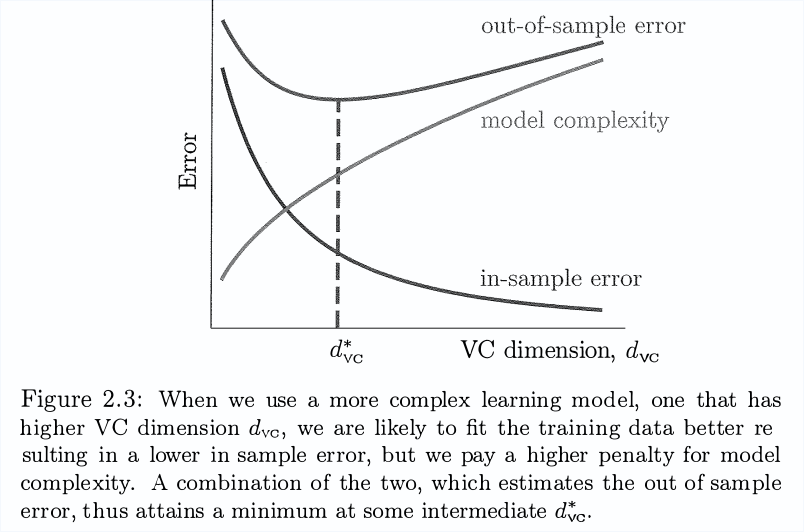
\includegraphics[width=.9\linewidth]{Training versus Testing (2)/screenshot_2018-09-12_19-20-23.png}
\end{center}

\subsubsection{The Test Set}
\label{sec:org7654224}
\begin{itemize}
\item One often estimates \(E_\text{out}\) by using a \textbf{test set} that the learning algorithm has not seen before
\begin{itemize}
\item Called \(E_\text{test}\)
\end{itemize}
\end{itemize}

\subsection{Approximation-Generalization Tradeoff}
\label{sec:org870ef91}
\subsubsection{Bias and Variance}
\label{sec:orgebbab53}
\begin{itemize}
\item The bias variance decomposition out-of-sample error is
\end{itemize}
\begin{equation}
  E_\text{out}(g^{(\mathcal D)}) = \mathbb E_{\pmb x} \big[ (g^{(\mathcal D)}(\pmb x) - f(\pmb x))^2 \big]
\end{equation}

\begin{itemize}
\item The function \(\bar g (\pmb x)\) can be interpreted in the following operational way
\begin{enumerate}
\item Generate many data sets \(\mathcal D_1, \dots, \mathcal D_K\)
\item Apply the learning algortihm to each data set obtaining final hypotheses \(g_1,\dots,g_K\).
\item The average function for any \(\pmb x\) is then estimated by \(\bar g(\pmb x) \approx \frac1K \sum_{k=1}^K g_k(\pmb x)\)
\end{enumerate}

\item The \textbf{bias} is \(\text{bias}(\pmb x) = (\bar g(\pmb x) - f(\pmb x))^2\)
\begin{itemize}
\item It measures how much the average function deviates from the target function
\end{itemize}

\item The \textbf{variance} is
\end{itemize}
\begin{equation}
	\text{var}(\pmb x)   = E_\mathcal D [(g^{\mathcal D}(x) - \bar g(\pmb x))^2]
\end{equation}
\begin{itemize}
\item Says how much the different hypotheses varies

\item Since bias and variance cannot be computed in a real model
\begin{itemize}
\item They are purly a conceptual tool used when developing a model
\end{itemize}
\end{itemize}

\subsubsection{The Learning Curve}
\label{sec:org341662d}
\begin{center}
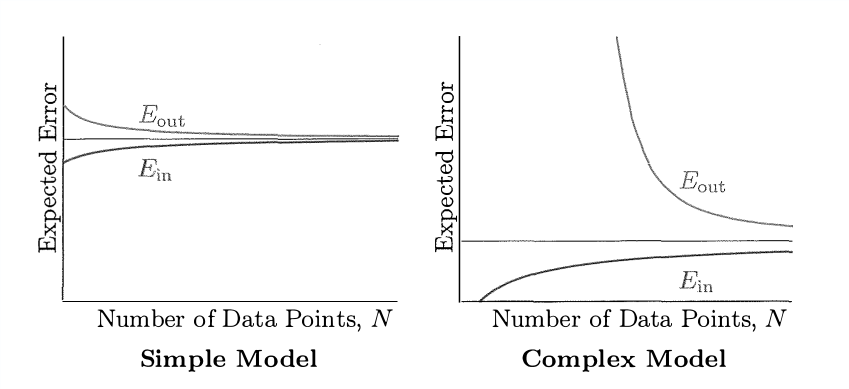
\includegraphics[width=.9\linewidth]{Training versus Testing (2)/screenshot_2018-09-12_20-08-30.png}
\end{center}

\begin{itemize}
\item For a simpler model the learning curves converge more quickly but to worse ultimate performance
\begin{itemize}
\item The in-sample error learning curve is increasing in \(N\)
\item The out-of-sample error learning curve is decreasing in \(N\)
\end{itemize}
\end{itemize}

\section{The Linear Model (3)}
\label{sec:org636cea2}
\subsection{Linear Regression}
\label{sec:org74ec40d}
\subsubsection{The algorithm}
\label{sec:org8162f98}
\begin{itemize}
\item The linear regression algorithm is based on minimizing the squared error between \(h(x)\) and \(y\)
\end{itemize}
\begin{equation}
  E_\text{out}(h) = \mathbb E[(h(\pmb x) - y)^2]
\end{equation}
where the expected value is taken with respect to the joint probability distribution \(P(x,y)\) 

\begin{itemize}
\item The goal is to find an hypothesis that achieves a small \(E_\text{out}(h)\)
\begin{itemize}
\item Since the distribution \(P(\pmb x, y)\) is unknown \(E_\text{out}(h)\) cannot be computed the in-sample version is therefore used instead
\end{itemize}
\end{itemize}
\begin{equation}
	E_\text{in}(h) = \frac{1}{n}\sum_{n=1}^N(h(\pmb x_n) - y_n)^2
\end{equation}

\begin{itemize}
\item In linear regression \(h\) takes the form of a linear combination of the components of \(x\) that is
\end{itemize}
\begin{equation}
  h(\pmb x) = \sum_{i=0}^dw_ix_i = \pmb w^T\pmb x
\end{equation}
where \(x_0 = 1\) an \(\pmb x \in \{1\} \times \mathbb R ^d\) as usual and \(\pmb w \in \mathbb R^{d+1}\) 

\begin{itemize}
\item For the special case of linear \(h\), it is very useful to have a matrix representation of \(E_\text{in}(h)\)
\begin{itemize}
\item First we define the data matrix \(X \in \mathbb R^{N \times (d+1)}\) to be the \(N \times (d+1)\) matrix whose rows are the inputs \(x_n\) as row vector
\item Define the target vector \(\pmb y \in \mathbb R^N\) to be the column vector whose components are the target values \(y_n\)
\end{itemize}
\end{itemize}

\begin{center}
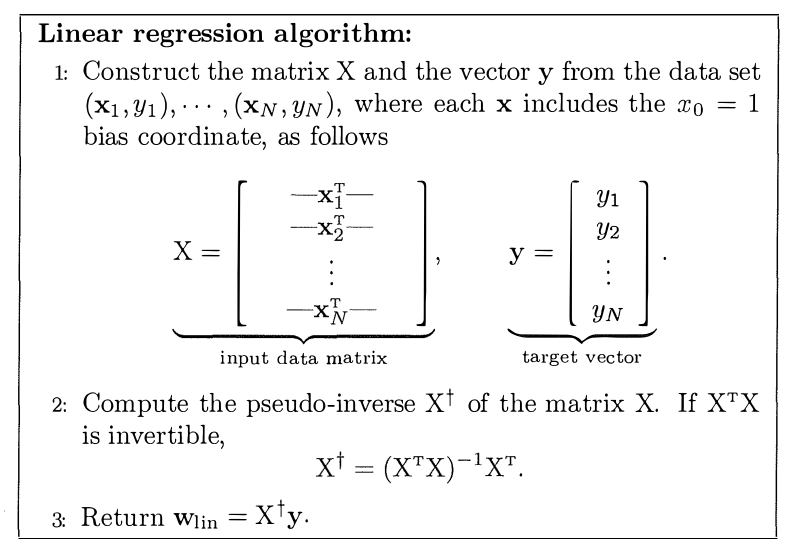
\includegraphics[width=.9\linewidth]{The Linear Model/screenshot_2018-08-28_14-54-58.png}
\end{center}
\subsection{Logistic Regression}
\label{sec:orgfddaa36}
\subsubsection{Predicting a Probability}
\label{sec:org6f539c7}
\begin{itemize}
\item To predict a probability we want something which restricts the output to the probability range \([0,1]\), one choice that accomplishes this goal is the logistic regression model
\end{itemize}
\begin{equation}
    h(\pmb x) = \theta(\pmb w^T \pmb x)
\end{equation}
\begin{itemize}
\item Where \(\theta\) is the \emph{logistic} function \(\theta(s) = \frac{e^s}{1+e^s}\) whose output is between 0 and 1
\begin{itemize}
\item The output can be interpret as a probability for a binary event
\item The logistic function \(\theta\) is referred to as a \textbf{soft threshold} in contrast to the \textbf{hard threshold} in classification
\item It is also called a \textbf{sigmoid}
\end{itemize}

\item When using Logistic Regression we are formally trying to learn the target function
\end{itemize}
\begin{equation}
  f(\pmb x) = \mathbb P [y=+1 \mid \pmb x]
\end{equation}

\begin{itemize}
\item The data given is generated by a noisy target \(P(y \mid \pmb x)\)
\end{itemize}
\begin{equation}
  \begin{equation*}
    P(y \mid \pmb x) = 
  		\begin{cases}
  			\mbox{$f(\pmb x)$} & \mbox{for $y=+1$} \\
  			\mbox{$1-f(\pmb x)$} & \mbox{for $y=-1$} 
  		\end{cases}
  \end{equation*}    
\end{equation}

\begin{itemize}
\item The standard \textbf{error measure} \(e(h(\pmb x),y)\) used in logistic regression is based how likely it is that we would get this output \(y\) from the input \(\pmb x\). if the target distribution \(P(y | \pmb x)\) was indeed captured by our hypothesis \(h(x)\).

\item The \textbf{error measure} is \(E_\text{in}(\pmb w) = \frac1N \sum_{n=1}^N\ln(1+e^{-y_n\pmb w^T x_n})\)
\end{itemize}

\subsubsection{Gradient Descent}
\label{sec:org3592f3f}
\begin{enumerate}
\item Batch Gradient Descent
\label{sec:orgc066748}
\begin{itemize}
\item Gradient descent is a general technique for minimize a twice differentiable function
\begin{itemize}
\item e.g. \(E_\text{in}(\pmb w)\) in logistic regression
\item You start somewhere and go the steepest way down the surface
\item You may end up in a local minima
\item When using a convex function such as \(E_{in}\) there is only one minima the global unique minimum
\end{itemize}

\item When steeping in a direction you need that the step \(\eta\) is not too small or too large
\end{itemize}
\begin{center}
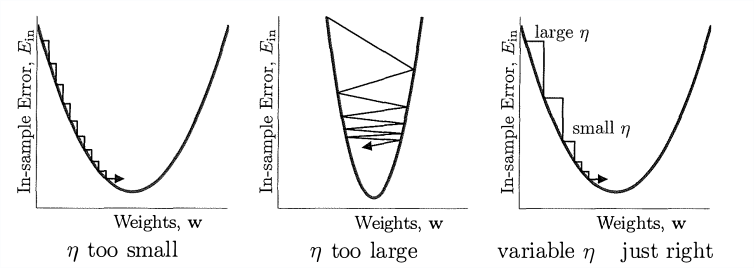
\includegraphics[width=.9\linewidth]{The Linear Model/screenshot_2018-09-03_17-19-24.png}
\end{center}
\begin{itemize}
\item You typically want to choose \(\eta_t = \eta || \bigtriangledown E_\text{IN} ||\) to obtain a good variable step size
\end{itemize}

\begin{center}
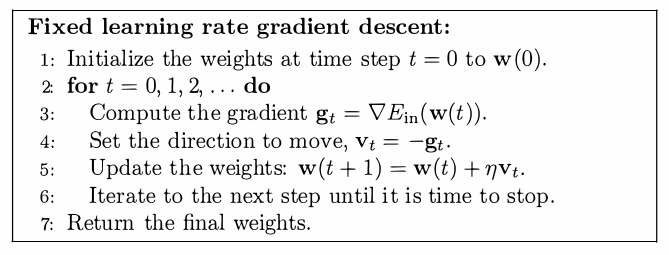
\includegraphics[width=.9\linewidth]{The Linear Model/screenshot_2018-09-03_17-24-49.png}
\end{center}
\begin{itemize}
\item A typical good choice for \(\eta\) is a fixed learning rate is around \(0.1\) the
\end{itemize}

\begin{center}
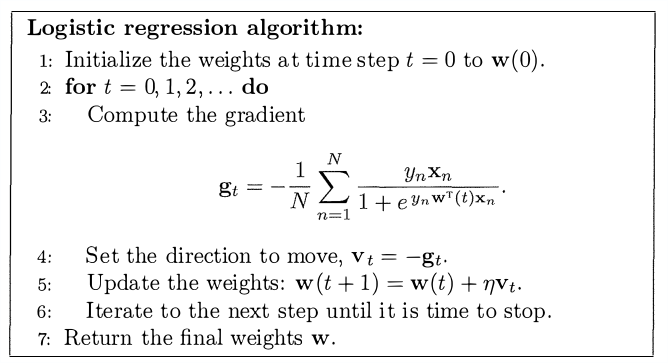
\includegraphics[width=.9\linewidth]{The Linear Model/screenshot_2018-09-03_17-28-37.png}
\end{center}

\begin{itemize}
\item \textbf{Initialization}
\begin{itemize}
\item Most of the time the initializing the initial weights as zeros works well
\item It is in general safer to initialize the weights randomly
\item Choosing each weight independently from a Normal distribution with zero mean and small variance usually works well
\end{itemize}

\item \textbf{Termination}
\begin{itemize}
\item A simple approach would be to set and upper limit on the number of iterations
\begin{itemize}
\item Does not guarantee anything on the quality of the final weights
\end{itemize}
\item A natural terminal criterion would be to stop ones \(||\pmb g_t||\) drops below a certain threshold
\begin{itemize}
\item Eventually this must happen but we do not know but we will now know when
\end{itemize}
\item For logistic regression a combination of the two termination conditions is used
\end{itemize}
\end{itemize}

\item Stochastic Gradient Descent (SGD)
\label{sec:org6a094de}
\begin{itemize}
\item A sequential version of Batch Gradient Decent
\begin{itemize}
\item Often beats the batch version in practise
\end{itemize}

\item Instead of considering the full batch gradient on all \(N\) training points, we consider a stochastic version of the gradient
\begin{enumerate}
\item Pick a training data point \((\pmb x_n, y_n)\) at uniformly random
\item Consider only the error on that point (in case of logistic regression)
\end{enumerate}
\end{itemize}
\begin{equation}
   e_n(w) = \ln ( 1+ e^{-y_n \pmb w^T \pmb x_n})
\end{equation}

\begin{itemize}
\item The gradient needed is
\end{itemize}
\begin{equation}
  \nabla e_n (\pmb w) = \frac{-y_n\pmb x_n}{1+e^{-y_n \pmb w^T \pmb x_n}}
\end{equation}
\begin{itemize}
\item The weight update is \(\pmb w \leftarrow \pmb w \cdot \eta \nabla e_n(\pmb w)\)
\end{itemize}
\end{enumerate}

\subsection{Nonlinear Transformation}
\label{sec:org593ac5f}
\subsubsection{The \(\mathcal Z\) space}
\label{sec:orgdd75e98}
\begin{figure}[htbp]
\centering
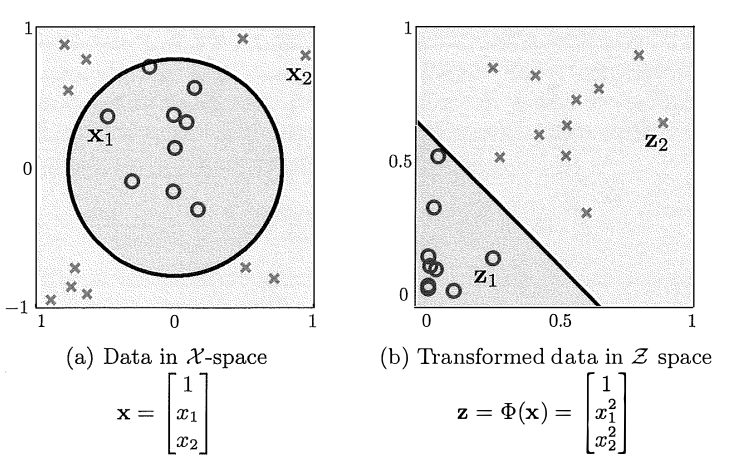
\includegraphics[width=.9\linewidth]{The Linear Model/screenshot_2018-09-03_18-22-01.png}
\caption{\label{fig:orgd93abf9}
Example of nonlinear transform}
\end{figure}
\begin{itemize}
\item Using a nonlinear transformation we can convert data which is not linear separable into data that is
\begin{itemize}
\item The space \(\mathcal Z\) generated is called the \textbf{feature space}
\item The transformation from the original space \(\mathcal X\) to \(\mathcal Z\) is called a \textbf{feature transform}
\end{itemize}

\item Any linear hypothesis \(\tilde h\) in \(\pmb z\) corresponds to a (possible nonlinear) hypothesis of
\(\pmb x\) given by \(h(\pmb x) = \tidle h (\theta(\pmb x))\) where \(\theta\) is a non linear transform
\begin{itemize}
\item The set of these hypothesis is denoted by \(\mathcal H_\theta\)
\end{itemize}
\end{itemize}

\begin{figure}[htbp]
\centering
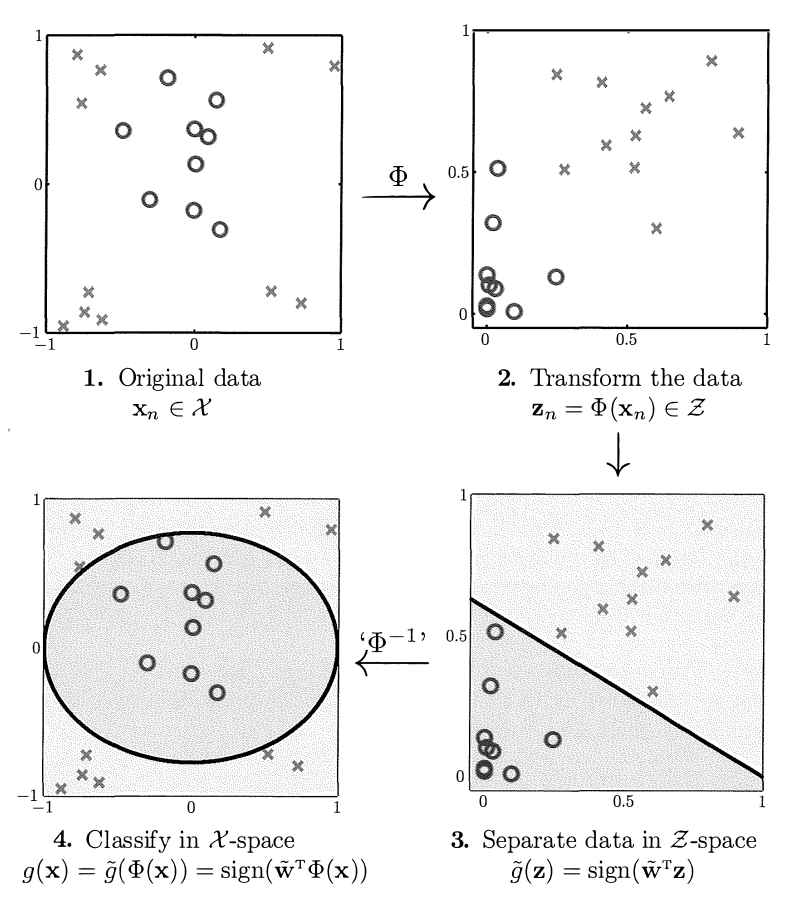
\includegraphics[width=.9\linewidth]{The Linear Model/screenshot_2018-09-03_18-28-08.png}
\caption{\label{fig:orgfd63357}
The nonlinear transform for separating non separable data.}
\end{figure}

\begin{itemize}
\item The feature transform \(\theta_Q\) is defined for degree-\(Q\) curves in \(\mathcal X\)
\begin{itemize}
\item It is called the Qth order polynomial transform
\end{itemize}
\end{itemize}
p- The power of the feature transform should be used with care, it may not be worth it to insist on linear separability and employ a highly complex surface
\begin{itemize}
\item It is sometime better to tolerate a small \(E_in\) than using a feature transform
\end{itemize}

\subsubsection{Computation and generalization}
\label{sec:orgdf85d3d}
\begin{itemize}
\item Computation is an issue because \(\theta_Q\) maps a two dimensional vector \(\pmb x\) to \(\tilde d = \frac{Q(Q+3)}2\) dimensions, which increases the memory and computational cost
\begin{itemize}
\item Things could get worse if \(\pmb x\) is in a higher dimension to begin with
\end{itemize}

\item The problem of generalization is another important issue
\begin{itemize}
\item We will have a weaker guarantee that \(E_\text{OUT}\) is small
\item It is sometime balanced  by the advantage we get in approximating the target better
\end{itemize}
\end{itemize}

\begin{center}
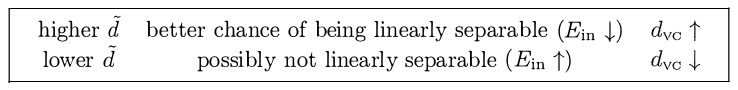
\includegraphics[width=.9\linewidth]{The Linear Model (3)/screenshot_2018-09-04_07-51-06.png}
\end{center}
\section{Multinomial/Softmax Regression}
\label{sec:org3ca051c}
\subsection{Setup}
\label{sec:orgb794184}
\begin{itemize}
\item Multinomial/Softmax Regression generalizes logistic regression to handle \(K\) classes instead of \(2\)
\begin{itemize}
\item A target value \(y\) is represented as a vector of length \(K\) with all zeroes except one which is called a one-in-\(K\) encoding
\item To store all the data points a matrix \(Y\) of size \(n \times K\) and the data matrix \(X\) is unchanged
\end{itemize}
\end{itemize}
\begin{equation}
X=\begin{pmatrix} 
1&- & x_1^T & - \\
\vdots & \vdots & \vdots \\
1&- & x_n^T & - \\
\end{pmatrix}\in \mathbb{R}^{n \times d}\quad\quad 
y=\begin{pmatrix}
- & y_1^T & -\\
- & \vdots &- \\
- & y_n^T & -\end{pmatrix}\in\{0,1\}^{n\times K}
\end{equation}

\begin{itemize}
\item To generalize to \(K\) classes we will use \(K\) weight vectors \(w_1,\dots,w_k\) each of length \(d\), one for each class.
\begin{itemize}
\item To classify data we can use the following algorith: Given data x, compute \(w_i^\intercal x\) for \(i=1,\dots, K\) and return the index of the largest value.
\item The list of weight vectors is packed into a matrix \(W\) of size \(d \times K\) by putting \(w_1\) in column one and so on.
\end{itemize}
\end{itemize}
$$
W=\begin{pmatrix} 
(w_1)_1  & \dots & (w_K)_1 \\
\vdots & \vdots & \vdots \\
(w_1)_d  & \dots & (w_K)_d \\
\end{pmatrix}\in \mathbb{R}^{d \times n}
$$
\begin{itemize}
\item This way we can compute the weighed sum for each class by the vector matrix product \(x^\intercal W\) and then pick argmax of that to do the classification. Pretty Neat!.

\item Numpy example
\end{itemize}
\begin{verbatim}
import numpy as np
# example with 3 classes and d = 10
W = np.random.rand(10, 3)
print('Shape w:', W.shape)
x = np.array([1., 2., 3., 4., 5., 6., 7., 8., 9., 10.0]).reshape(10, 1)
print('Shape x:', x.shape)
model_predictions = x.T @ W
print('model (unnormalzed log) predictions: - picke the larger one\n', model_predictions)
\end{verbatim}

\subsection{Probabilistic Outputs}
\label{sec:org79c8d68}
\begin{itemize}
\item Given a set of model parameters \(W\) and a data point \(x\) we want \(P(y=i\mid x, W)\) for \(i=1,\dots K\).

\item \textbf{Softmax} is used in our probabilistic model
\begin{itemize}
\item It takes as input a vector of length \(K\) and outputs another vector of the same length \(K\), that is a mapping from the \(K\) input numbers into \(K\) \textbf{probabilities}
\end{itemize}
\end{itemize}
\begin{equation}
\textrm{softmax}(x)_j =
\frac{e^{x_j}}
{\sum_{i=1}^K e^{x_i}}\quad
\textrm{ for }\quad j = 1, \dots, K.
\end{equation}
\begin{itemize}
\item where \(\textrm{softmax}(x)_j\) denote the \(j\)'th entry in the vector.
\begin{itemize}
\item The denominator acts as a normalization term that ensures that the probabilities sum to one
\item The exponentiation ensures all numbers are positive.
\item We get the following derivatives:
\end{itemize}
\end{itemize}
\begin{equation}
\frac
{\partial \;\textrm{softmax}(x)_i}
{\partial x_j} =
(\delta_{i,j} - \textrm{softmax}(x)_j)
\textrm{softmax}(x)_i\quad\quad\text{where}\quad\quad
\delta_{ij}=\begin{cases}1 &\text{if }i=j\\
0 & \text{else}
\end{cases}
\end{equation}

\begin{itemize}
\item The following is our probabilistic model
\end{itemize}
\begin{equation}
p(y \mid x, W) =
\textrm{softmax}(W^\intercal x) =
 \left \{
\begin{array}{l l}
 \textrm{softmax}(W^\intercal x)_1 & \text{ if } y = e_1,  \\
 \vdots & \\
 \textrm{softmax}(W^\intercal x)_K & \text { if } y = e_K.
\end{array}
\right.
\end{equation}

\begin{itemize}
\item We compute the likelihood of the data given a fixed matrix of parameters.
\begin{itemize}
\item The notation \([z]\) for the indicator function
\end{itemize}
\end{itemize}
$$
P(D \mid W) =
\prod_{(x,y)\in D}
\prod_{j=1}^K
\textrm{softmax}(W^\intercal x)_j^{[y_j=1]}
=
\prod_{(x,y)\in D}
y^\intercal
\textrm{softmax}(W^\intercal x)
.
$$

\begin{itemize}
\item This way of expressing is the same as we did for logistic regression.
\end{itemize}

\subsection{The Negative Log Likelihood}
\label{sec:org8691ae0}
\begin{itemize}
\item The negative log likelihood of the data is minimized instead of maximizing the likelihood of the data and get a pointwise sum.
\end{itemize}
\begin{align}\textrm{NLL}(D\mid W) &=
-\sum_{(x,y)\in D}
\sum_{j=1}^K
[y_j=1]
\ln (\textrm{softmax}(W^\intercal x)_j)
\\
&=-\sum_{(x,y)\in D}
y^\intercal
\ln (\textrm{softmax}(W^\intercal x))
\end{align}


\begin{itemize}
\item In the last summation only one value will be nonzero:
\end{itemize}
\begin{equation}
  - \ln \textrm{softmax}(z)_j = \ln \left( \frac{e^{z_j}}{\sum_{i=1}^d e^{z_i}}\right) = - (z_j - \ln \sum_{i=1}^d e^{z_i})
\end{equation}

\begin{itemize}
\item The insample error is defined to be  \(E_\textrm{in} = \frac{1}{|D|} \textrm{NLL}\)
\begin{itemize}
\item Cannot be solved for a 0 analytically
\item To apply stochastic mini-batch gradient descent as for Logistic Regression all you really need is the gradient of the negative log likelihood function.
\begin{itemize}
\item The gradient is a \textbf{simple} generalization of the one used in logistic regression.
\item There is a set of parameters for each of \(K\) classes, \(W_j\) for \(j=1,\ldots,K\)
\item The gradient is
\end{itemize}
\end{itemize}
\end{itemize}
$$
\nabla \textrm{NLL}(W) =
-X^\intercal
(Y - \textrm{softmax}(XW)),
$$

\subsection{Implementation Issues}
\label{sec:orgb8164d9}
\subsubsection{Numerical Issues with Softmax}
\label{sec:org09cd7ff}
\begin{itemize}
\item There are some numerical issues with the softmax function
\end{itemize}

$$
\textrm{softmax}(x)_j = \frac{e^{x_j}}{\sum_{i=1}^K e^{x_i}} \textrm{ for } j=1,\ldots,K.
$$
\begin{itemize}
\item This is because this is a sum of exponentials and exponentiation of numbers tend to make them very large giving numerical problems.

\item The problematic part is the logarithm of the sum of exponentials.
\item We can move \(e^c\) for any constant \(c\) outside the sum easily, that is:
\end{itemize}
$$
\ln\left(\sum_i e^{x_i}\right) =
\ln\left(e^c \sum_i e^{x_i-c}\right) =
c + \ln\left(\sum_i e^{x_i -c}\right).
$$

\begin{itemize}
\item We need to find a good \(c\), and we choose \(c = \max_i x_i\)
\item Since \(e^{x_i}\) is the dominant term in the sum. We are less concerned with values being inadvertently rounded to zero since that does not
\end{itemize}

\subsubsection{One in k encoding}
\label{sec:org172793e}
\begin{itemize}
\item Representing a number \(k\) in \([1,\dots,k]\) as a vector of length may \(K\) be quite cumbersome.
\begin{itemize}
\item In general the input labels will just be a list/vector of numbers between 1 and k.
\item It is your job to transform it into a matrix if needed.
\item But this will be a very sparse matrix.
\item It may be worthwhile to consider whether it is possible to implement the operations with the matrix Y without actually creating the matrix.
\end{itemize}
\end{itemize}

\subsubsection{Always check your shapes}
\label{sec:orgff5560e}
\begin{itemize}
\item If the shapes dont fit then
\begin{itemize}
\item If trying to implement softmax it is very useful to ensure you have full control over the shapes of all matrices and vectors you use.
\item If there is a shape mismatch then clearly there is a larger issue.
\item Checking shapes is a very efficient heuristic for catching bugs.
\end{itemize}
\end{itemize}

\subsubsection{Bias Variable}
\label{sec:orgba13b6c}
\begin{itemize}
\item If you need a Bias variable \(b\) (remember \(w^\intercal x + b\)) for each class you need to add a columns of ones to \(X\) and make \(W\) a \(d+1 \times K\) matrix.
\end{itemize}

\section{Overfitting (4)}
\label{sec:org7d23c93}
\subsection{When Does Overfitting Occur?}
\label{sec:orgb8bac2a}
\subsubsection{General}
\label{sec:org9e09ea0}
\begin{figure}[htbp]
\centering
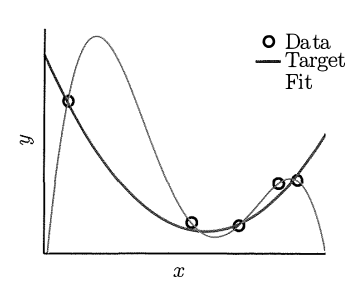
\includegraphics[width=.9\linewidth]{Overfitting (4)/screenshot_2018-09-17_10-02-37.png}
\caption{\label{fig:org49557a1}
Example of overfitting}
\end{figure}
\begin{itemize}
\item The main case of overfitting is when you pick the hypothesis with lower \(E_{in}\) and it results in higher \(E_{out}\)
\begin{itemize}
\item Means that \(E_{in}\) alone is no longer a good guide for learning
\item A typical overfitting scenario is when a complex model uses its addition degress of freedom to "learn" the noise
\end{itemize}
\end{itemize}

\subsubsection{Catalysts for Overfitting}
\label{sec:org4d73b5f}
\begin{center}
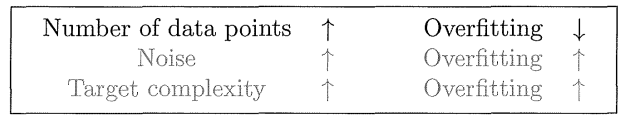
\includegraphics[width=.9\linewidth]{Overfitting (4)/screenshot_2018-09-17_10-16-04.png}
\end{center}
\begin{itemize}
\item On a finite data set the algorithm inadvertently uses some of the degrees of freedom to fit the noise
\begin{itemize}
\item Can result in overfitting and a spurious final hypothesis
\end{itemize}

\item There are two types of noise which that algorithm cannot differentiate
\begin{itemize}
\item \textbf{Deterministic noise} will not change if the dataset was generated again
\begin{itemize}
\item Is different depending on which model we use
\item Related to the bias
\end{itemize}
\item \textbf{Stochastic noise} will change if the dataset was generated again
\begin{itemize}
\item Related to the variance
\end{itemize}
\end{itemize}
\end{itemize}

\subsection{Regularization}
\label{sec:org3cdf7d4}
\subsubsection{General}
\label{sec:org61e80a7}
\begin{itemize}
\item \textbf{Regularization} is a way to combat overfitting
\begin{itemize}
\item Constraints the learning algorithm to improve out-of-sample error
\item Especially when noise is present
\end{itemize}

\item A view of regularization is thought the VC bound, which bounds \(E_\text{out}\) using a model complexity penalty \(\Omega(\mathcal H)\):
\end{itemize}
\begin{equation}
    E_\text{out}(h) \leq E_\text{in}(h) + \Omega(\mathcal H) \ \text{for all } h \in \mathcal H
\end{equation}
\begin{itemize}
\item We are better off fitting the data using a simple \(\mathcal H\)

\item Instead on minimizing \(E_\text{in}(h)\) alone one minimizes the combination of \(E_\text{in}(h)\) and \(\Omega(h)\)
\begin{itemize}
\item Avoids overfitting by constraining the learning algorithm to fit data well using a simple hypotheses
\end{itemize}
\end{itemize}

\subsubsection{A Soft Order Constraint}
\label{sec:org5179c37}
\begin{itemize}
\item A \textbf{Soft Order Constraint} can be defined as the hypotheses set
\end{itemize}
\begin{equation}
    \mathcal{C}=\{h \mid h(\pmb x) = \pmb x ^T\pmb x, \pmb w^T \pmb w \leq C\}
\end{equation}
\begin{itemize}
\item Solving for \(\pmb w_\text{reg}\):
\begin{itemize}
\item If \(\pmb w_\text{lin}^T \pmb w_\text{lin} \leq C\) then \(\pmb w_\text{reg} = \pmb w_\text{lin}\) since \(\pmb w_\text{lin} \in \mathcal H(C)\)
\item If \(\pmb w_\text{lin} \notin \mathcal H(C)\) then not only is \(\pmb w_\text{lin}^T \pmb w_\text{lin} \leq C\) but \(\pmb w_\text{lin}^T \pmb w_\text{lin} = C\)
\begin{itemize}
\item The weights \(\pmb w\) must lie on the surface of thee \$sphere \(\pmb w^T \pmb w = C\)
\end{itemize}
\end{itemize}

\item If \(\pmb w_\text{reg}\) is to be optimal then for some positive parameter \(\lambda_C\)
\end{itemize}
\begin{equation}
  \nabla E_\text{in}(\pmb w_\text{reg}) = - 2 \lambda_C\pmb w_\text{reg}
\end{equation}
\begin{itemize}
\item \(\nabla E_\text{in}\) must be parallel to \(\pmb w_\text{reg}\)
\end{itemize}

For some \(\lambda_C > 0\) \(\pmb w_\text{reg}\) locally minimizes
\begin{equation}
    E_\text{in}(\pmb w) + \lambda_CW^TW
\end{equation}

\subsubsection{Weight Decay and Augmented Error}
\label{sec:org36592bc}
\begin{center}
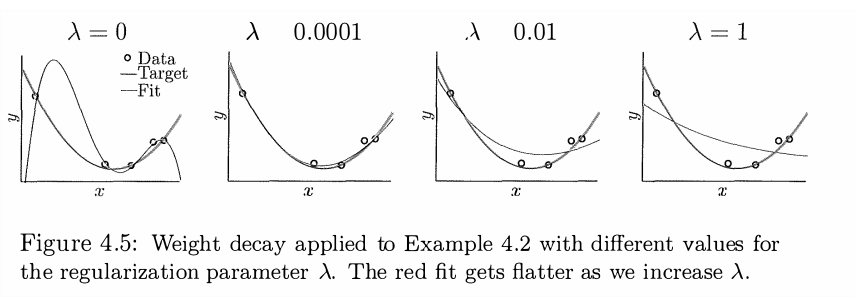
\includegraphics[width=.9\linewidth]{Overfitting (4)/screenshot_2018-09-18_08-20-44.png}
\end{center}
\begin{itemize}
\item The \textbf{augmented error} is defined as
\end{itemize}
\begin{equation}
  E_\text{aug}(\pmb w) = E_\text{in}(\pmb w) + \lambda \pmb w^T \pmb w
\end{equation}
\begin{itemize}
\item where \(\lambda \geq 0\) is now a free parameter

\item The penalty term enforces a trade-off between making the in-sample error small and making the weights small
\begin{itemize}
\item Is also known as the \textbf{weight decay}
\item Minimizing the error together with the decay is known as \textbf{ridge regression}
\end{itemize}

\item If we can find the optimal \(\lambda^*\) we can minimize the out-of-sample error

\item In general the \textbf{augmented error} for a hypothesis set \(h \in \mathcal H\) is
\end{itemize}
\begin{equation}
    E_\text{aug}(h,\lambda,\Omega) = E_\text{in}(h) + \frac\lambda N \Omega(h)
\end{equation}
\begin{itemize}
\item For weight decay \(\Omega(h) = \pmb w^T\pmb w\)
\begin{itemize}
\item The need for regularization goes down as the number of data points goes up
\end{itemize}
\end{itemize}

\subsubsection{Choosing a Regularizer}
\label{sec:orga172df2}
\begin{center}
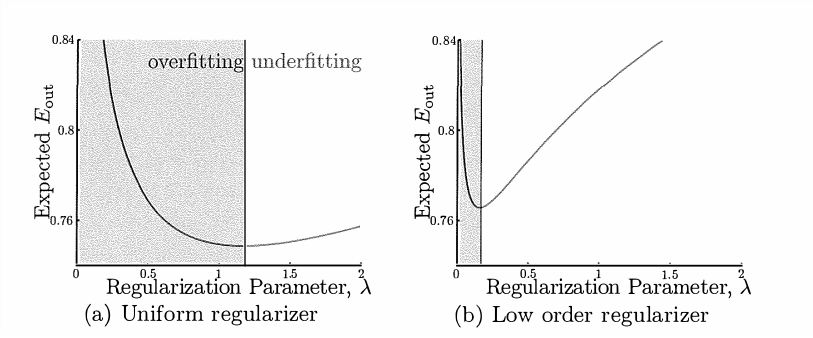
\includegraphics[width=.9\linewidth]{Overfitting (4)/screenshot_2018-09-18_08-32-17.png}
\end{center}

\begin{itemize}
\item A uniform regularizer, is a penalizes the weights equally
\begin{itemize}
\item encourages all weights to be small uniformly
\item Example \(\Omega_\text{unif}(\pmb w)= \sum_{q=0}^{15}w_q^2\)
\end{itemize}
\item A lower-order regularizer
\begin{itemize}
\item Pairs more attention to the higher order weights
\item Example \(\Omega_\text{low}(\pmb w)= \sum_{q=0}^{15}qw_q^2\)
\end{itemize}

\item The price paid for overfitting is generally more severe than underfitting
\item The optimal  value for the regularization parameter increases with noise
\item No regularizer will be ideal for all settings
\begin{itemize}
\item Not even specific settings
\item The entire burden rest on picking the right \(\lambda\)
\end{itemize}
\item Some for of regularization is necessary as learning is quite sensitive to stochastic and deterministic noise
\end{itemize}

\subsection{Validation}
\label{sec:orgaf2f4f1}
\subsubsection{The Validation Set}
\label{sec:org8bb81ff}
\begin{itemize}
\item \textbf{Validation} tries to estimate the out-of-sample error directly

\item The idea of a \textbf{validation set} is almost identical to that of a test set
\begin{itemize}
\item A subset of the data is removed and not used in training
\item Will be used to make certain choice in the learning process
\begin{itemize}
\item Therefore not a test set
\end{itemize}
\end{itemize}

\item The \textbf{validation set} is created and used in the following way
\begin{enumerate}
\item Partition the data set \(\mathcal D\) using into a training set \(\mathcal D_\text{train}\) of size \((N-K)\) and a validation set \(\mathcal D_\text{val}\) of size \(K\)
\begin{itemize}
\item Any partitioning method which does not depend on the data will do
\end{itemize}
\item Run the learning algorithm using the training set \(\mathcal D_\text{train}\) to obtain a final hypothesis \(g^- \in \mathcal H\)
\item The validation error is then computed for \(g\) using the validation set \(\mathcal D_\text{val}\)
\end{enumerate}
\end{itemize}
\begin{equation}
  E_\text{val}(g^-)=\frac1K\sum_{\pmb x_n \in \mathcal D_\text{val}} e(g^-(\pmb x_n),y_n)
\end{equation}
\begin{itemize}
\item where \(e(g(\pmb x),y)\) is the pointwise error measure

\item The validation error is an \emph{unbiased} estimate of \(E_\text{out}\) because the final hypothesis \(g^-\) was created independently of the validation set
\begin{itemize}
\item The expected error of \(E_\text{val}\) is \(E_\text{out}\)
\item If \(K\) is neither too small nor too large \(E_\text{val}\) is a good estimate of \(E_\text{out}\)
\item A rule of thumb in practise is to set \(K=\frac N5\)
\end{itemize}

\item We should not output \(g^-\) we should output \(g\) which is trained on the entire hypothesis set \(D\)
\begin{itemize}
\item To estimate \(E_\text{out}\) we use that \(E_\text{out}(g) \leq E_\text{out}(g^-)\) because of the learning curve
\begin{itemize}
\item Is not rigorously proved
\item It is just very likely
\end{itemize}
\end{itemize}
\end{itemize}

\subsubsection{Model Selection}
\label{sec:orgc695f2a}
\begin{center}
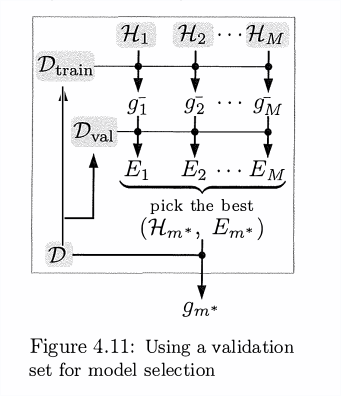
\includegraphics[width=.9\linewidth]{Overfitting (4)/screenshot_2018-09-18_09-48-43.png}
\end{center}
\begin{itemize}
\item The most important use of validation is for \textbf{model selection}
\begin{itemize}
\item Choosing linear or nonlinear, polynomial or not\ldots{}
\item It could any choice that affects the learning process
\end{itemize}

\item It can be used to estimate the out-of-sample error for more than one model, suppose we have \(M\) models \(\mathcal H_1, \dots, \mathcal H_M\) 
\begin{itemize}
\item Validation can be used to select one of these models
\item Use the training set \(\mathcal D_\text{train}\) to learn the final hypothesis \(g^-_m\) for each model
\item Evaluate each model on the validation set to obtain the validation errors \(E_1,\dots,E_M\) where
\end{itemize}
\end{itemize}
\begin{equation}
  E_m = E_\text{val}(g^-_m); \text{ for } m = 1,\dots,M
\end{equation}
\begin{itemize}
\item Then just select the model with the lowest validation error.
\item For suitable \(K\) even \(g^-_{m*}\) is better than in-sample selection of the model
\item The validation error can also be used to select a lambda by using \((\mathcal H, \lambda_1),(\mathcal H, \lambda_2),\dots,(\mathcal H \lambda_M)\) as our \(M\) different models
\item The more one uses the validation set to fine tune the model the more the it becomes like the training set
\end{itemize}

\subsubsection{Cross Validation}
\label{sec:orged2f05d}
\begin{center}
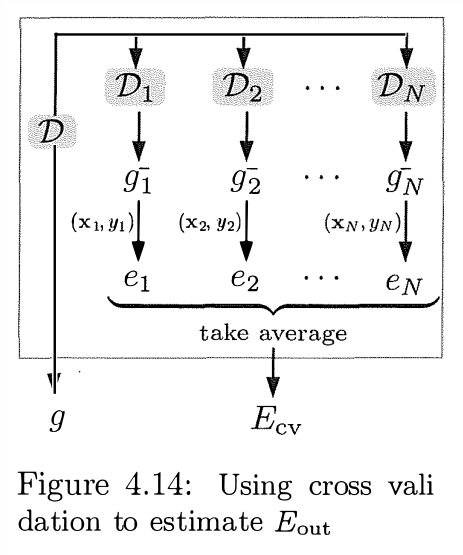
\includegraphics[width=.9\linewidth]{Overfitting (4)/screenshot_2018-09-18_20-20-44.png}
\end{center}

\begin{itemize}
\item There are \(N\) ways to partition a set of size \(N-1\) and a validation set of size \(1\). Let
\end{itemize}
\begin{equation}
  \mathcal D_n = (\pmb x_1, y_1), \dots, (\pmb x_{n-1}, y_{n-1}), (\pmb x_{n+1}, y_{n+1}), \dots, (\pmb x_N, y_N)
\end{equation}
\begin{itemize}
\item The final hypothesis learned from \(\mathcal D_n\) is denoted \(g_n^-\)
\item Let \(e_n\) be the error made by \(g_n^-\) on its validation set which is just a single point \(\{(\pmb x_n, y_n)\}\)
\item The cross validation estimate is the average value of the \(e_n\text{'s}\)
\end{itemize}
\begin{equation}
  E_\text{cv}=\frac1N \sum_{n=1}^Ne_n
\end{equation}

\begin{itemize}
\item \textbf{Theorem 4.4.} \(E_\text{cv}\) is an unbiased estimate of \(\bar E_\text{out}(N-1)\)
\begin{itemize}
\item The expectation of the model performance, \(\mathbb E[E_\text{out}])\), over data set of size \(N-1\)
\end{itemize}

\item The cross validation estimate will on average be an upper estimate for the out-of-sample error: \(E_\text{out}(g) \leq E_\text{cv}\)

\item Cross validation can be for model selection for a given set of models \(\mathcal H_1, \dots, \mathcal H_M\) in the same way as validation set
\end{itemize}

\begin{center}
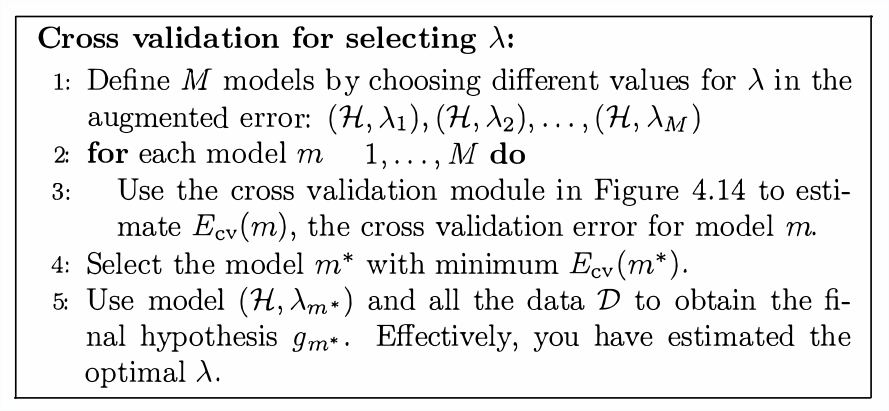
\includegraphics[width=.9\linewidth]{Overfitting (4)/screenshot_2018-09-18_20-42-49.png}
\end{center}

\begin{itemize}
\item To get cross validation for \(M\) models and a data set \(D\) of size \(N\) is requires \(MN\) rounds of learning
\item If one could analytically obtain \(E_\text{cv}\) it would be a big bonus
\begin{itemize}
\item Analytical results are hard to come
\item An analytical method exists for linear models
\end{itemize}

\item The cross validation estimate can be analytically computed as
\end{itemize}
\begin{equation}
  E_\text{cv} = \frac1N\sum_{n=1}^N(\frac{\hat y_n-y_n}{1-H_nn(\lambda)})^2
\end{equation}
\begin{itemize}
\item where \(H(\lambda)=Z(Z^TZ+ \lambda I)^{-1}Z^T\)
\end{itemize}

\section{Support Vector Machines}
\label{sec:org550c73c}
\subsection{Notation}
\label{sec:orgbf940fe}
\begin{itemize}
\item The classifier considered will be a linear classifier for a binary classification problem with labels \(y\) and features \(x\)
\begin{itemize}
\item \(x \in \{-1,1\}\)
\item The classifier with parameters \(w\) and \(b\)  is written as
\end{itemize}
\end{itemize}
\begin{equation}
  h_{w,b}(x)=g(w^Tx+b)
\end{equation}
\begin{itemize}
\item where g = 1 if \(z \geq 0\) and \(g(z)= -1\) otherwise
\end{itemize}

\subsection{Functional and geometric margins}
\label{sec:orgb267d89}
\begin{itemize}
\item Given a training example \((x^{(i)},y^{(i)})\), the \textbf{functional margin} of \((w,b)\) is defined with respect to the training example
\end{itemize}
\begin{equation}
  \hat \gamma^{(i)}=y^{(i)}(w^Tx+b)
\end{equation}
\begin{itemize}
\item A large functional margin represents a confident and a correct prediction
\item Given a training set \(S = \{(x^{(i)},y^{(i)}); i=1,\dots,m\}\) the functional margin of \((w,b)\) with respect to \(S\) is
\end{itemize}
\begin{equation}
  \hat \gamma = ‎‎‎‎‎‎\min_{i=1,\dots,m} \hat \gamma^{(i)}
\end{equation}

\begin{itemize}
\item The \textbf{geometric margin} of \((w,b)\) with respect to a training example \((x^{(i)},y^{(i)})\) to be
\end{itemize}
\begin{equation}
	\gamma^{(i)} = y{(i)} \Bigg( \bigg( \frac w{||w||} \bigg)^T x^{(i)} + \frac b{||w||}  \Bigg)
\end{equation}
\begin{itemize}
\item If \(||w|| == 1\) then the functional margin equals the geometric margin
\item Given a training set \(S = \{(x^{(i)},y^{(i)}); i=1,\dots,m\}\) the \textbf{geometric margin} of \((w,b)\) with respect to \(S\) is
\end{itemize}
\begin{equation}
	\gamma = ‎‎‎‎‎‎\min_{i=1,\dots,m} \gamma^{(i)}
\end{equation}

\subsection{The optimal margin classifier}
\label{sec:org29d7950}
\begin{itemize}
\item The problem of finding a decision boundary which has the largest geometric margins is the following optimisation problem
\end{itemize}
\begin{equation}
  \begin{split} 
    \max_{\gamma,w,b} \ &\gamma\\
    \text{s.t.} \ & y^{(i)}(w^Tx^{(i)}+b) \geq \gamma, \ i= 1, \dots, m \\
    &||w|| = 1
  \end{split}
\end{equation}
\begin{itemize}
\item this can be be turned into the following problem using functional margins and rescaling it
\end{itemize}
\begin{equation}
  \begin{split} 
   \max_{\gamma,w,b} \ &\frac12 ||w||^2\\ 
    \text{s.t.} \ & y^{(i)}(w^Tx^{(i)}+b) \geq 1, \ i= 1, \dots, m \\
  \end{split}
\end{equation}
\begin{itemize}
\item It is called the \textbf{optimal margin classifier}
\end{itemize}

\subsection{Lagrange duality}
\label{sec:org851c9bd}
\begin{itemize}
\item Consider a problem of the following form:
\end{itemize}
\begin{equation}
  \begin{split} 
    \text{min}_w &\ f(w)  \\
    \text{s.t.} &\ h_i(w) = 0, \ i=1,\dots,l
  \end{split}
\end{equation}
\begin{itemize}
\item The \textbf{Lagrangian} is defined to be
\end{itemize}
\begin{equation}
  \mathcal L(w,\beta) = f(w) + \sum_{i=1}^l\beta_ih_i(w)
\end{equation}
\begin{itemize}
\item The \(\beta_i\)'s are called the \textbf{Lagrange multipliers}
\begin{itemize}
\item We would the find and set \(\mathcal L\)'s partial derivatives to zero
\end{itemize}
\end{itemize}
\begin{equation}
  \frac{\partial \mathcal L}{\partial w_i} = 0; \frac{\partial \mathcal L}{\partial \beta_i} = 0
\end{equation}
and solve for \(w\) and \(\beta\) 

\begin{itemize}
\item The \textbf{primal} optimization problem is the following
\end{itemize}
\begin{equation}
  \begin{split} 
    \text{min}_w &\ f(w)  \\
    \text{s.t.} &\ g_i(w) \leq 0, \ i=1,\dots, k
								&\ h_i(w) = 0, \ i=1,\dots,l
  \end{split}
\end{equation}

\begin{itemize}
\item The primal optimization problem is solved by defining the \textbf{generalized Lagrangian}
\end{itemize}
\begin{equation}
  \mathcal L (w,\alpha,\beta) = f(w) + \sum_{i=1}^k \alpha_ig_i(w) + \sum_{i=1}^k \beta_ih_i(w)
\end{equation}
\begin{itemize}
\item The \(\alpha_i\)'s and \(\beta_i\)'s are the Lagrange multipliers.
\item Consider the quantity
\end{itemize}
\begin{equation}
    \theta_\mathcal{P}(w) = \max_{\alpha, \beta: \alpha_i \geq 0} \mathcal L (w,\alpha,\beta)
\end{equation}
\begin{itemize}
\item If \(w\) violates any of the primal constraints then one should be able to verify that
\end{itemize}
\begin{equation}
    \theta_\mathcal P (w) = \infty
\end{equation}
\begin{itemize}
\item If \(w\) does not violate the constraints then \(\theta_\mathcal P(w) = f(w)\) and therefore the minimization problem
\end{itemize}
\begin{equation}
  \min_w\theta_\mathcal P(w) = \min_w \max_{\alpha,\beta:\alpha_i \geq 0} \mathcal L (w,\alpha,\beta)
\end{equation}
\begin{itemize}
\item is the same as the original problem
\begin{itemize}
\item the objective is called the \textbf{value} of the primal problem and is denoted \(p* = \min_w \theta _ \mathcal P (w)\)
\end{itemize}

\item If one define
\end{itemize}
\begin{equation}
    \theta_D(\alpha,\beta) = \min_w \ \mathcal L (w,\alpha,\beta)
\end{equation}
\begin{itemize}
\item The "\(\mathcal D\)" subscript stands for dual
\begin{itemize}
\item This can be used to pose the \textbf{dual} optimization problem
\end{itemize}
\end{itemize}
\begin{equation}
  \max_{\alpha,\beta: \alpha_i  \geq 0} \theta_\mathcal D (\alpha, \beta) = \max_{\alpha,\beta: \alpha_i  \geq 0} \min_w \ \mathcal L (w,\alpha,\beta)
\end{equation}
\begin{itemize}
\item Which is exactly the same as the primal problem, except the order of the min and max has been exchanged
\begin{itemize}
\item The solution to the dual problem is defined as \(d^*\)
\item It holds that \(d^* \leq p^*\)
\end{itemize}

\item The KKT conditions on \(w^*\), \(\alpha^*\) and \(\beta^*\)
\end{itemize}
\begin{center}
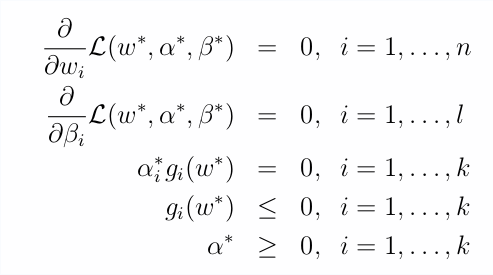
\includegraphics[width=.9\linewidth]{Support Vector Machines/screenshot_2018-09-24_17-52-15.png}
\end{center}

\begin{itemize}
\item If some \(w^*\), \(\alpha^*\), \(\beta^*\) satisfy the KKT conditions they are also a solution to the primal and dual problems
\end{itemize}

\subsection{Optimal margin classifiers}
\label{sec:org85ddfc0}
\begin{itemize}
\item By using the KKT conditions obtain the following optimization problem, which gives us a decision boundary with the largest margins:
\end{itemize}
\begin{center}
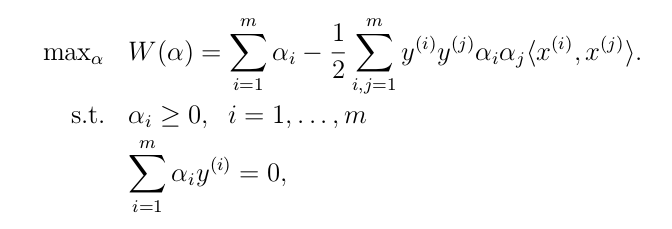
\includegraphics[width=.9\linewidth]{Support Vector Machines/screenshot_2018-09-25_07-46-53.png}
\end{center}

\begin{itemize}
\item Where \(w= \sum_{i=1}^m a_iy^{(i)}x^{(i)}\) 
\begin{itemize}
\item The prediction \(w^Tx+b\) can also be written as
\end{itemize}
\end{itemize}
\begin{center}
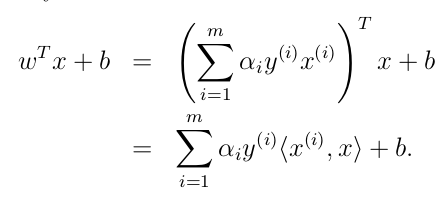
\includegraphics[width=.9\linewidth]{Support Vector Machines/screenshot_2018-09-25_07-50-38.png}
\end{center}
\begin{itemize}
\item Where post of the inner products will be zero except for the support vectors
\end{itemize}

\subsection{Kernels}
\label{sec:org44d901c}
\begin{itemize}
\item Given a feature mapping \(\phi\) we define the corresponding \textbf{Kernel} to be
\end{itemize}
\begin{equation}
  K(x,z) = \phi(x)^T\phi(z)
\end{equation}
\begin{itemize}
\item Everywhere we previously had \(\langle x, z \rangle\) we could simple replace it with \(K(x,z)\) and the algorithm would now be learning using the features \(\phi\)

\item The \textbf{Gaussian kernel} which corresponds to an infinite dimensional feature mapping \(\phi\)
\end{itemize}
\begin{equation}
  K(x,z) = \exp(-\frac{||x-z||^2}{2\sigma^2})
\end{equation} 

\begin{itemize}
\item The matrix called the \textbf{Kernel matrix} is defined from some \(m\) data points \(\{x^{(1)}, \dots, x^{(m)}\}\) as the m-by-m matrix \(K\) where the \((i,j)\) entry is given by \(K_{ij}=K(x^{(i)},y^{(i)})\)

\item \textbf{Theorem (Mercer).} Let \(K: \mathbb R^n \times \mathbb R^n \mapsto \mathbb R\) be given. Then for \(K\) to be a valid (Mercer) kernel, it is necessary and sufficient that for any \(\{x^{(1)}, \dots, x^{(m)}\}\), \(m < \infty\), the corresponding kernel matrix is symmetric positive semi-definite
\end{itemize}

\subsection{Regularization and the non-separable case}
\label{sec:orgb6d8784}
\begin{itemize}
\item To make the algorithm work for non-linearly separable datasets and being less sensitive to outliers, the optimization can be reformulated as follows using regularization:
\end{itemize}
\begin{center}
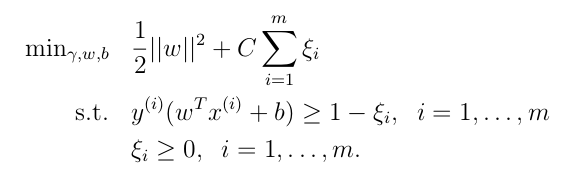
\includegraphics[width=.9\linewidth]{Support Vector Machines/screenshot_2018-09-25_08-30-17.png}
\end{center}
\begin{itemize}
\item Which means that examples are now permitted to have a functional margin less than 1

\item By using some of the KKT conditions one can obtain the following dual form of problem
\end{itemize}
\begin{center}
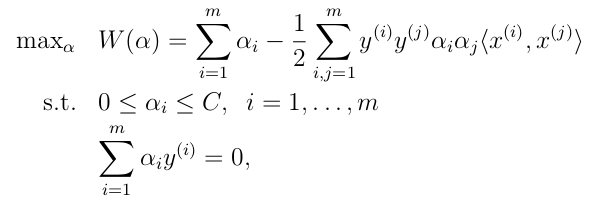
\includegraphics[width=.9\linewidth]{Support Vector Machines/screenshot_2018-09-25_08-36-39.png}
\end{center}

\subsection{The SMO algorithm}
\label{sec:org8f1a36c}
\subsubsection{General}
\label{sec:org2a1afef}
\begin{itemize}
\item The SMO algorithm gives an efficient way of solving the dual problem arising from the derivation of the SVM
\end{itemize}

\subsubsection{Coordinate ascent}
\label{sec:org29f6a64}
\begin{figure}[htbp]
\centering
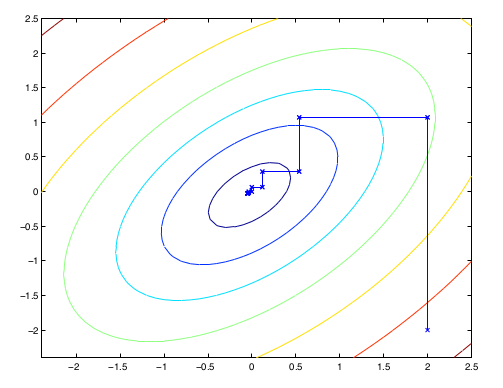
\includegraphics[width=.9\linewidth]{Support Vector Machines/screenshot_2018-09-25_08-44-24.png}
\caption{\label{fig:org9fc88ba}
Coordinate ascent example}
\end{figure}

\begin{itemize}
\item If one is trying to solve the unconstrained optimization problem
\end{itemize}
\begin{equation}
  \max_\alpha W(\alpha_1,\alpha_2, \dots,\alpha_m)
\end{equation}
\begin{itemize}
\item One can use the algorithm called \textbf{coordinate ascent:}
\end{itemize}
\begin{center}
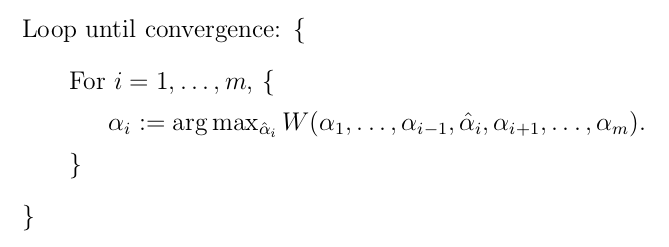
\includegraphics[width=.9\linewidth]{Support Vector Machines/screenshot_2018-09-25_08-47-20.png}
\end{center}
\begin{itemize}
\item Where one holds all the variables fixed except some \(a_i\)
\end{itemize}

\subsubsection{SMO}
\label{sec:orgee0b8f5}
\begin{itemize}
\item The SMO algorithm does the following
\end{itemize}
\begin{center}
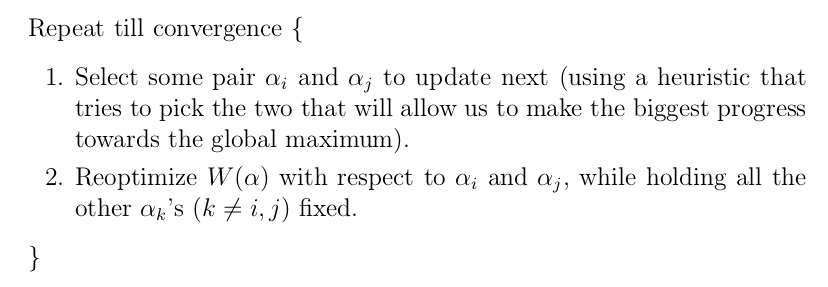
\includegraphics[width=.9\linewidth]{Support Vector Machines/screenshot_2018-09-25_09-00-29.png}
\end{center}
\begin{itemize}
\item To test for convergence, one can test whether the KKT conditions are satisfied within some \emph{tol}
\begin{itemize}
\item The tol is the convergence tolerance parameter normally set around \(0.01\) to \(0.001\)
\end{itemize}
\end{itemize}
\section{Deep Feedforward Networks}
\label{sec:org92d738a}
\subsection{General}
\label{sec:org4021950}
\begin{itemize}
\item \textbf{Deep feedforward networks} are quintessential deep learning models 
\begin{itemize}
\item The goal of a feedforward network is to approximate some function \(f^*\)
\item It defines a mapping \(\pmb y = f(\pmb x; \pmb \theta)\) and learns the value of the parameters \(\pmb \theta\) that result in the best function approximation
\end{itemize}

\item It is called \textbf{feedforward} since information flows through the function being evaluated from \(\pmb x\), through intermediate computations used to define \(f\) and finally to the output \(\pmb y\)
\begin{itemize}
\item When feedforward neural networks are extended to include feedback connections, they are called \textbf{recurrent neural networks}
\end{itemize}

\item They are called \textbf{networks} because they typically are represented by composing together many different function
\begin{itemize}
\item It is associated with a DAG describing ow the functions are composed together
\item The different functions are called \textbf{layers}
\item The overall length of the function chain gives the \textbf{depth} of the model
\item The final layer is called the \textbf{output layer}
\item During the training we drive \(f(\pmb x)\) to match \(f^*(\pmb x)\)
\item The training data provides us with noisy, approximate examples of \(f^*(\pmb x)\) evaluated at different training points
\item The training data does not say what each individual layers should do
\begin{itemize}
\item That is the training algorithms job
\item They are called \textbf{hidden layers}
\end{itemize}
\item The dimensionality of these hidden layers determines the \textbf{width} of the model
\end{itemize}

\item The strategy of deep learning is the feature transform \(\phi\)
\begin{itemize}
\item We have a model \(=f(\pmb x; \pmb \theta, \pmb w) = \phi(\pmb x, \pmb \theta)^\top \pmb w\)
\item We have the parameters \(\pmb \theta\) that we use to learn \(\phi\) from a broad class of functions
\item We have the parameters \(\pmb w\) that map from \(\phi(\pmb x)\) to the desired output
\end{itemize}

\item Training a feedforward network requires making many of the same design decisions as are necessary for a linear model:
\begin{itemize}
\item Choosing the optimizer
\item The cost function
\item The form of the output units.
\end{itemize}
\end{itemize}

\subsection{Gradient-Based Learning}
\label{sec:org8264ab3}
\subsubsection{General}
\label{sec:orgb16f43e}
\begin{itemize}
\item The non-linearity of a neural network causes most interesting loss functions to become non-convex
\begin{itemize}
\item It means that NNs are usually are trained by using iterative, gradient-based optimizes that merely drive the cost function to a very low value
\item It is important to initialize all weights to random values becomes of the error function being non-convex, when using stochastic gradient descent 
\begin{itemize}
\item The biases may be initialized to zero or a small positive values
\end{itemize}
\end{itemize}
\end{itemize}

\subsubsection{Cost Functions}
\label{sec:org4103bbf}
\begin{enumerate}
\item General
\label{sec:org7755dcf}
\begin{itemize}
\item Cost functions for neural network are more or less the same as those for other models, such as linear models
\begin{itemize}
\item The total cost function used to train a neural network will often combine one of the primary cost functions with a regularization term
\end{itemize}
\end{itemize}

\item Learning Conditional Distributions with Maximum Likelihood
\label{sec:orgf79d5c8}
\begin{itemize}
\item Most NNs are trained using maximum likelihood
\begin{itemize}
\item The cost function is simply the NLL which is equivalently described as the cross-entropy between the training data and the model distribution
\item This cost function is given by:
\end{itemize}
\end{itemize}
\begin{center}
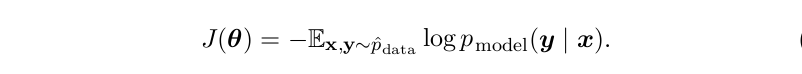
\includegraphics[width=.9\linewidth]{Deep Feedforward Networks/screenshot_2018-09-30_16-58-07.png}
\end{center}
\begin{itemize}
\item The advantage of deriving the cost function from maximum likelihood is that it removes the burden of designing cost functions for each model
\begin{itemize}
\item Specifying a model \(p(\pmb y \mid \pmb x)\) automatically determines a cost function \(\log p(\pmb y \mid \pmb x)\)
\end{itemize}

\item Instead of learning a full probability distribution \(p(\pmb y \mid \pmb x; \pmb \theta)\), we often want to learn just one conditional statistic of \(\pmb y\) given \(\pmb x\)
\begin{itemize}
\item Such as predicting the mean of \(\pmb y\) given the predictor \(f(\pmb x; \pmb \theta)\)
\end{itemize}
\end{itemize}

\item Learning Conditional Statistics
\label{sec:orgff421f1}
\begin{itemize}
\item Instead of learning a full probability distribution \(p(\pmb y \mid \pmb x; \pmb \theta)\) one often want to learn just one condition statistic of \(\pmb y\) given \(\pmb x\)
\begin{itemize}
\item Such as predicting the mean of \(\pmb y\)
\item The cost function can be viewed as being a \textbf{functional} rather than just a function
\begin{itemize}
\item A mapping from functions to real numbers
\end{itemize}
\item The cost functional can be designed to have its minimum occur at some specific function we desire
\end{itemize}

\item Solving the optimization problem
\end{itemize}
\begin{equation}
  f^*=\arg\min_f\mathbb E_{\pmb x, \pmb y \sim p_{data}}||\pmb y - f(\pmb x)||^2
\end{equation}
yields
\begin{equation}
  f^*(\pmb x) = \mathbb E_{\pmb y \sim p_{data}(\pmb y \mid x)[\pmb y]}
\end{equation}

\begin{itemize}
\item The following function yields a function that predicts the \emph{median} value of \(\pmb y\) for each \(\pmb x\)
\end{itemize}
\begin{equation}
	f^*=\arg\min_f\mathbb E_{\pmb x, \pmb y \sim p_{data}}||\pmb y - f(\pmb x)||_1
\end{equation}
\begin{itemize}
\item This cost function is commonly call \textbf{mean absolute error}
\end{itemize}
\end{enumerate}

\subsubsection{Output Units}
\label{sec:org6b57cbe}
\begin{enumerate}
\item General
\label{sec:orgc939eac}
\begin{itemize}
\item The choice of cost function is tightly coupled with the choice of output unit
\begin{itemize}
\item Most of the time one simply uses the cross-entropy between the data distribution and the model distribution
\item The choice of how to represent the output determines the cross-entropy function
\item Any kind of neural network that may be used as output can also be used as a hidden unit
\end{itemize}

\item The hidden features is defined by \(\pmb h = f(\pmb x ; \pmb \theta)\)
\begin{itemize}
\item The role of the output layer is to provide some additional transformation from the features to complete the task that the network must perform
\end{itemize}
\end{itemize}

\item Linear Units for Gaussian Output Distributions
\label{sec:org672659c}
\begin{itemize}
\item Linear units is an output unit based on an affine transformation with no non-linearity
\begin{itemize}
\item Given features \(\pmb h\), a layer of linear output units produces a vector \(\hat{\pmb y}= \pmb W^T \pmb h + b\)
\item Linear output layers are often used to produce the mean of a conditional Gaussian distribution
\end{itemize}
\end{itemize}
\begin{equation}
  p(\pmb y \mid \pmb x) = \mathcal N(\pmb y; \hat{\pmb y}, \pmb I)
\end{equation}
\begin{itemize}
\item Maximizing the log-likelihood is the equivalent to minimizing the mean squared error
\end{itemize}
\end{enumerate}

\subsection{Hidden Units}
\label{sec:orgbbe8257}
\subsubsection{General}
\label{sec:orga3b7d30}
\begin{itemize}
\item Some valid hidden units are not differentiable at all input points
\begin{itemize}
\item Such as \(g(z)=\max\{0,z\}\)
\item Solved by using the right or left differential
\end{itemize}
\end{itemize}

\subsubsection{Rectified Linear Units and Their Generalizations}
\label{sec:org75dc01b}
\begin{itemize}
\item Rectified linear units use the activation function \(g(z) = \max\{0,z\}\)
\begin{itemize}
\item Easy to optimize because they are similar to linear units
\begin{itemize}
\item Only difference is that a rectified unit outputs zero across half its domain
\end{itemize}
\end{itemize}

\item Rectified linear units are typically used on top of an affine transformation
\end{itemize}
\begin{equation}
  \pmb h = g(\pmb W^\top \pmb x + \pmb b)
\end{equation}
\begin{itemize}
\item When initializing the parameters of the affine transformation it can be a good pratise to set all elements of \(\pmb b\) to a small positive value
\item A drawback to rectified linear units is that they cannot learn via gradient based methods on examples for which their activation is zero
\begin{itemize}
\item Some generalizations of rectified linear units guarantee that they receive gradient everywhere
\end{itemize}

\item \textbf{Maxout units} generalize rectified linear units further
\begin{itemize}
\item Instead of applying an element-wise function \(g(z)\) maxout units divide \(\pmb z\) into groups of \(k\) values
\item Each maxout unit the outputs the maximum element of one of these groups
\end{itemize}
\end{itemize}
\begin{equation}
  g(\pmb z)_i = \max_{j\in \mathbb G^{(u)}} z_j
\end{equation}
\begin{itemize}
\item where \(\mathbb G^{(I)}\) is the set of indices into the inputs for group \(i\)

\item A maxout unit can be seen as learning the activation function itself rather than just the relationship between units
\end{itemize}

\subsubsection{Logistic Sigmoid and Hyperbolic Tangent}
\label{sec:orgab863cc}
\begin{itemize}
\item The widespread saturation of sigmoid units can make gradient-based learning very difficult
\begin{itemize}
\item Their use as hidden units in feedforward networks are discouraged
\item Training using the \(tanh\) function for hidden layers are easier
\end{itemize}
\end{itemize}

\subsection{Architecture Design}
\label{sec:org4db176b}
\subsubsection{General}
\label{sec:orgaa5e4d8}
\begin{itemize}
\item \textbf{Architecture} refers to the overall structure of the network
\begin{itemize}
\item How many units it should have
\item How these units should be connected to each other
\end{itemize}

\item Most NNs are organized into groups of units called layers
\begin{itemize}
\item They are often arranged in a chain structure where each layer is a function of the layer that preceded it
\item The ith layer is given by
\end{itemize}
\end{itemize}
\begin{equation}
  h^{(i)} = g^{(i)}(\pmb W ^{(i)T}\pmb h^{(i)} + \pmb b^{(i)})
\end{equation}
\begin{itemize}
\item where the first layer uses \(x\) instead of \(h^{(i)}\)

\item In chain based architectures, the main architectural considerations are to choose the the depth of the network and the width of each layer 
\begin{itemize}
\item The ideal network architecture for a task must be found via experimentation guided by monitoring the validation set error.
\end{itemize}
\end{itemize}

\subsubsection{Universal Approximation Properties and Depth}
\label{sec:org1f9154f}
\begin{itemize}
\item The universal approximation theorem means that regardless of what function we are trying to learn, we know that a large multi layered perceptron will be able to represent this function.
\begin{itemize}
\item However, we are not guaranteed that the training algorithm will be able to learn that function
\item Learning it can fail for two different reasons
\begin{enumerate}
\item The optimization algorithm used for training may not be able to find the value of the parameters corresponds to the desired function
\item The training algorithm might choose the wrong function due to overfitting
\end{enumerate}
\end{itemize}

\item Feedforward networks provide a universal system for representing functions, in the sense that, given a function, there exists a feedforward network that approximates the function.
\begin{itemize}
\item There is no universal procedure for examining a training set of specific examplesd and choosing a function that will generalize to point not in the training set
\end{itemize}

\item The universal approximation theorem says that there exists a network large enough to achieve any degree of accuracy we desire, but the theorem does not say how large this network will be.

\item A feedforward network with a single layer is sufficient to represent any function, but the layer may be infeasibly large and may fail to learn and generalize correctly.
\begin{itemize}
\item In many circumstances, using deeper models can reduce the number of units required to represent the desired function and can reduce the amount of generalization error
\end{itemize}

\item The number of linear regions carved out by a deep rectifier network with \(d\) inputs, depth \(l\), and \(n\) units per hidden layer is
\end{itemize}
\begin{center}
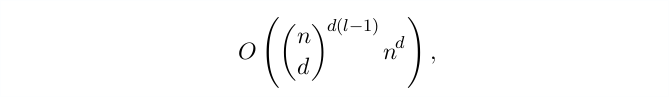
\includegraphics[width=.9\linewidth]{Deep Feedforward Networks/screenshot_2018-10-01_17-14-50.png}
\end{center}

\begin{itemize}
\item Choosing a deep model encodes a very general belief that the function we want to learn should involve composition of several simpler functions.
\end{itemize}

\subsubsection{Other Architectural Considerations}
\label{sec:orge05a8dc}
\begin{itemize}
\item The layers need not be connected in a chain, but it is the most common practice.
\begin{itemize}
\item Many architectures build a main chain but then add extra architectural features to it
\begin{itemize}
\item Such as skip connections going from layer i to layer i + 2 or higher.
\end{itemize}
\item These skip connections make it easier for the gradient to flow from output layers to layers nearer the input.
\end{itemize}

\item A key consideration of architecture design is how to connect a pair of layers to each other
\begin{itemize}
\item The default way is having every input unit connected to every output unit
\item Strategies for reducing the number of connections reduce the number of parameters and the amount of computation required to evaluate the network,
\begin{itemize}
\item They are often highly problem-dependent.
\end{itemize}
\end{itemize}
\end{itemize}

\subsection{Back-Propagation and Other Differentiation Algorithms}
\label{sec:org1097e2b}
\subsubsection{General}
\label{sec:orgfd78d2b}
\begin{itemize}
\item \textbf{Forward propagation} is when the inputs \(\pmb x\) provide initial information that then propaget up to the hidden units at each layer and finally produces an output \(\hat{\pmb y}\)
\begin{itemize}
\item During training it can continue onward until it produces a scalar cost \(J(\pmb \theta)\)
\end{itemize}

\item The \textbf{back-propagation} algorithm (\textbf{backprop}) allows the information from the cost to flow backwards through the network in order to compute the gradient
\begin{itemize}
\item It is used to compute the gradient, another algorithm is used to do the learning e.g. stochastic gradient descent
\end{itemize}
\end{itemize}

\subsubsection{Computational Graphs}
\label{sec:org17ea0d8}
\begin{figure}[htbp]
\centering
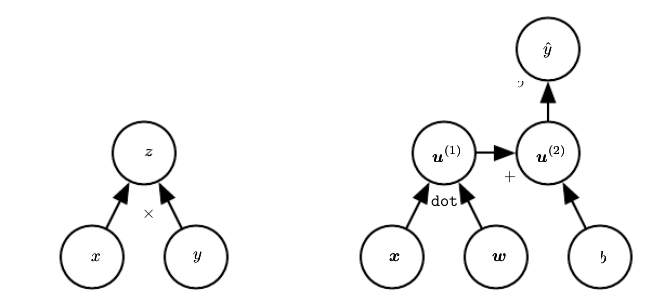
\includegraphics[width=.9\linewidth]{Deep Feedforward Networks/screenshot_2018-10-01_17-49-44.png}
\caption{\label{fig:orgb08084f}
Computational Graph Examples}
\end{figure}

\begin{itemize}
\item An \textbf{operation} is a simple function of one or more variables
\begin{itemize}
\item Defined to return only a single output variable
\end{itemize}

\item The graph language is accompanied by a set of allowable operations
\begin{itemize}
\item If a variables \(y\) is computed by applying an operation to a variable \(x\), then there is drawn a directed edge from \(x\) to \(y\)
\item The output node is sometimes annotated with the name of the operation applied
\end{itemize}
\end{itemize}

\subsubsection{Chain Rule of Calculus}
\label{sec:org234078f}
\begin{itemize}
\item Back-propagation computes the chain rule, with a specific order of operations that is highly efficient
\item The chain rule can generalize beyond the scalar case suppose that \(\pmb x \in \mathbb R^m, \pmb y \in \mathbb R^n\), \(g\) maps from \(\mathbb R^m\) to \(\mathbb R^n\), and \(f\) maps from \(\mathbb R^n\) to \(R\). If \(\pmb y = g(\pmb x)\) and \(z = f(\pmb y)\), then
\end{itemize}
\begin{center}
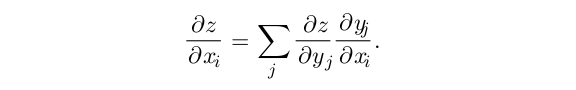
\includegraphics[width=.9\linewidth]{Deep Feedforward Networks/screenshot_2018-10-01_17-55-43.png}
\end{center}
\begin{itemize}
\item In vector notation, this may equivalently be written as
\end{itemize}
\begin{center}
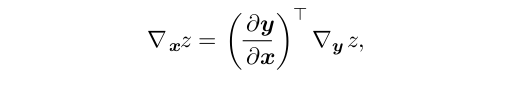
\includegraphics[width=.9\linewidth]{Deep Feedforward Networks/screenshot_2018-10-01_17-56-15.png}
\end{center}
\begin{itemize}
\item where \(\frac{\partial \pmb y}{\partial \pmb x}\)  is the \(n \times m\) Jacobian matrix of \(g\)

\item The back-propagation algorithm consists of performing Jacobian-gradient product given by the chain rule for each operation in the graph
\item The back-propagation algorithm is typically applied to tensors of arbitrary dimensionality
\begin{itemize}
\item Is exactly the same as back-propagation with vector conceptually
\item Denoting a gradient of a value \(z\) with respoect to a tensor \$s.
\end{itemize}
\item To denote the gradient of a value z with respect to a tensor \(\pmb X\), we write \(\nabla_{\pmb X} z\)
\begin{itemize}
\item The indices into \(\pmb X\) have multiple coordinates
\end{itemize}

\item The chain rule for tensors:
\end{itemize}
\begin{center}
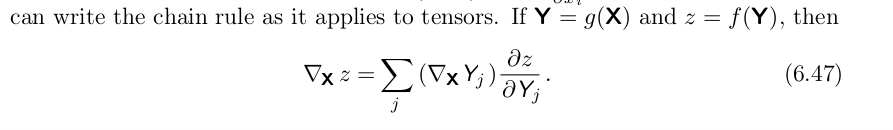
\includegraphics[width=.9\linewidth]{Deep Feedforward Networks/screenshot_2018-10-01_18-22-42.png}
\end{center}

\subsubsection{Recursively Applying the Chain Rule to Obtain Backprop}
\label{sec:org9c45613}
\begin{itemize}
\item Given a scalar \(u^{(n)}\) which is the quantity whose gradient we want to obtain with respect to all the \(n_i\) input nodes \(u^{(1)}\) to \(u^{(n_i)}\)
\begin{itemize}
\item We wish to compute \(\frac{\partial u^{(n)}}{\partial u^{(i)}}\) for \(i \in \{1,2,\dots,n_i\}\)
\item In backprop \(u^{(n)}\) will be the cost associated with an example or a minibatch
\item \(u^{(1)}\) to \(u^{(n_i)}\) correspond to the parameters of the model
\item The nodes of the graph is assumed to be order in such a way that we can compute their output one after the other
\item Each node \(u^{(i)}\) is associated with an operation \(f^{(i)}\) and is computed by evaluating the function
\end{itemize}
\end{itemize}
\begin{equation}
  u^{(i)} = f(\mathbb A ^{(i)})
\end{equation}
\begin{itemize}
\item where \(\mathbb A ^{(i)}\) is the set of all nodes that are parents of \(u^{(i)}\)
\end{itemize}
\begin{center}
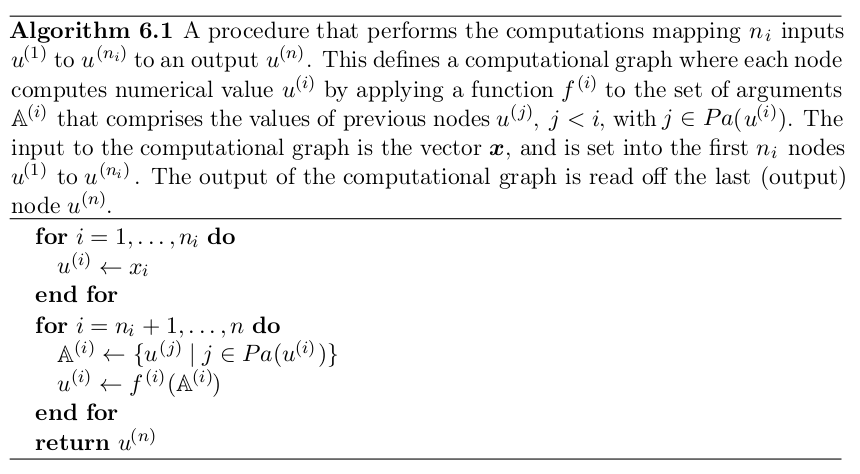
\includegraphics[width=.9\linewidth]{Deep Feedforward Networks/screenshot_2018-10-02_08-04-33.png}
\end{center}

\begin{itemize}
\item The forward propagation computation is put in a graph \(\mathcal G\)
\begin{itemize}
\item In order to perform back-propagation, one can constructs a computational graph that depends on \(\mathcal G\) and add to it an extra set of nodes
\begin{itemize}
\item These form a subgraph \(\mathcal B\) with one node per node of \(\mathcal G\)
\item Computation in \(\mathcal B\) proceeds in the reverse of the order of computation in \(\mathcal G\)
\item Each node of \(\mathcal B\) computes the derivative \(\frac{\partial u^{(n)}}{\partial u^{i}}\) associated with the forward graph node \(u^{(i)}\) using the chain rule
\end{itemize}
\item The subgraph \(\mathcal B\) contains one edge for each edge for each edge of \(\mathcal G\)
\begin{itemize}
\item The edge from \(u^{(j)}\) to \(u^{(i)}\) is associated with the computation of \(\frac{\partial u^{(i)}}{\partial u ^{(j)}}\)
\item The dot product is performed for each node between the gradient already computed with respect to nodes \(u^{(i)}\) that are children of \(u^{(j)}\) and the vector containing the partial derivatives \(\frac{\partial u^{(i)}}{\partial u ^{(j)}}\) for the same children nodes
\end{itemize}
\end{itemize}

\item The amount of computation required for performing back-propagration scales linearly with the number of edges in \(\mathcal G\)
\end{itemize}

\begin{center}
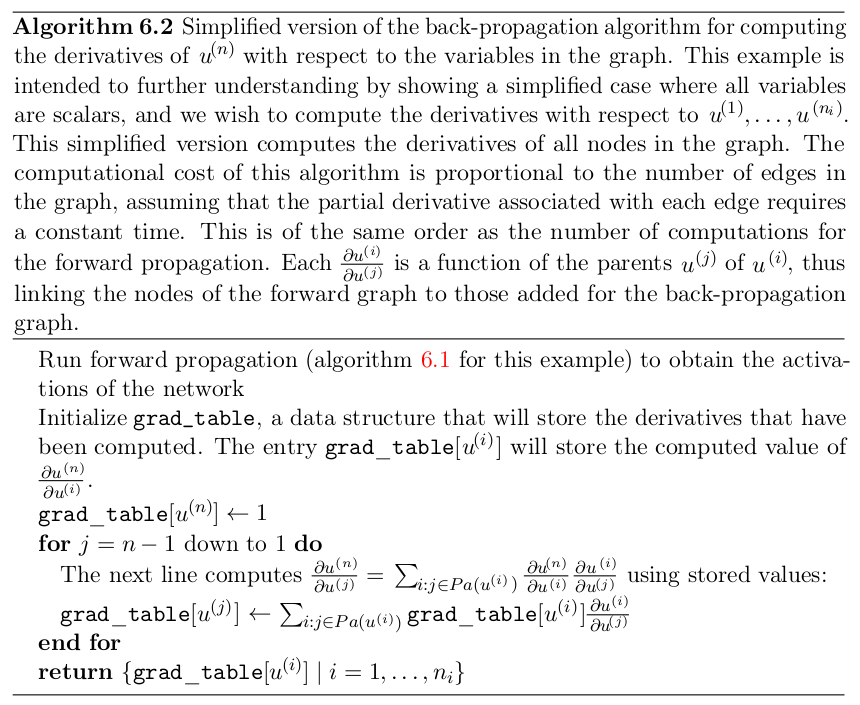
\includegraphics[width=.9\linewidth]{Deep Feedforward Networks/screenshot_2018-10-02_08-18-42.png}
\end{center}

\subsubsection{Back-Propagation Computation in Fully-Connected MLP}
\label{sec:org60a1b2c}
\begin{center}
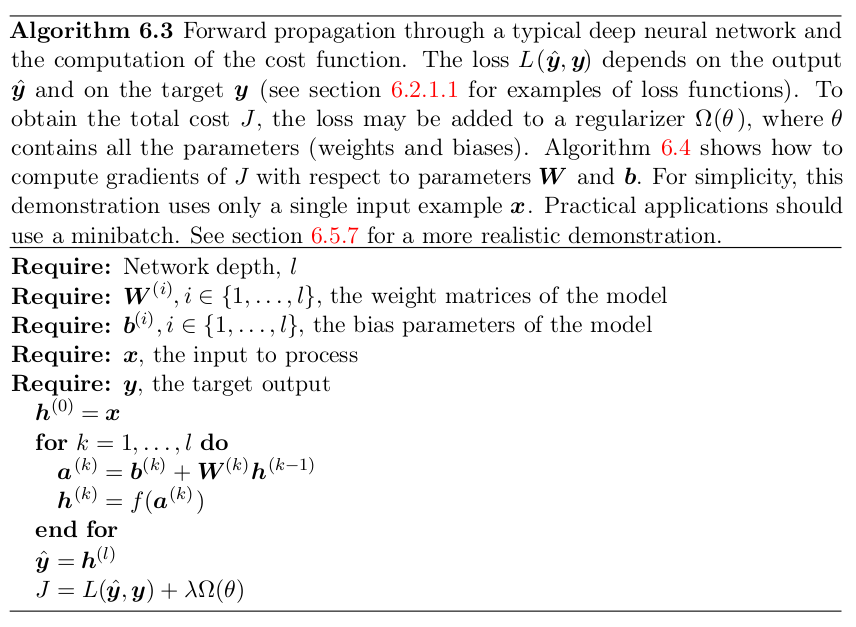
\includegraphics[width=.9\linewidth]{Deep Feedforward Networks/screenshot_2018-10-02_08-22-46.png}
\end{center}

\begin{center}
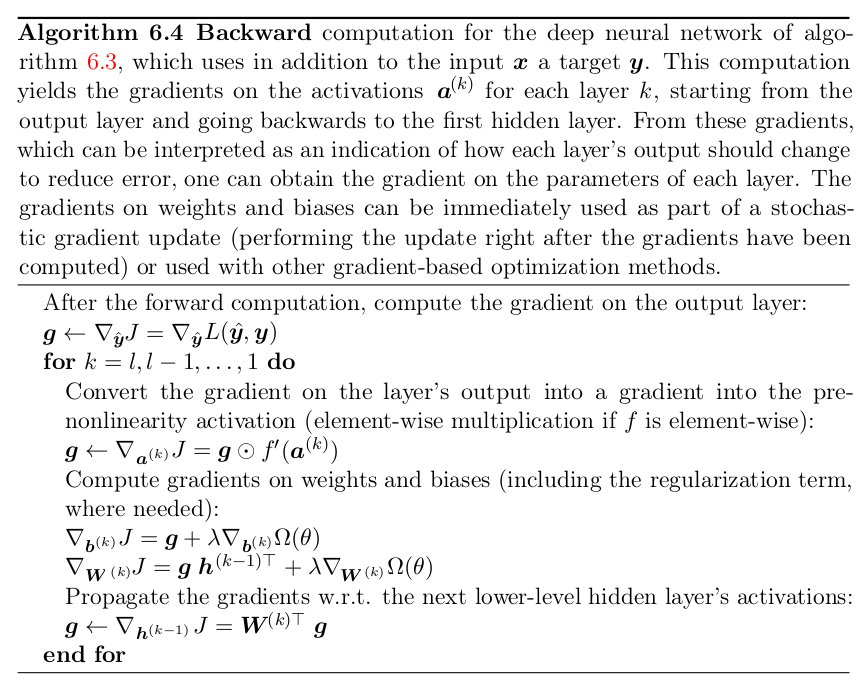
\includegraphics[width=.9\linewidth]{Deep Feedforward Networks/screenshot_2018-10-02_08-23-03.png}
\end{center}

\subsubsection{Symbol-to-Symbol Derivatives}
\label{sec:org8eec260}
\begin{itemize}
\item \textbf{Symbolic Representations} is algebraic expressions and computational graphs that both operate on symbols, or variables that do not have specific values.

\item Some approaches to back-propagation take a computational graph and a set of numerical values for the inputs to the graph, then return a set of numerical values describing the gradient at those input values.
\begin{itemize}
\item This is called "symbol-to-number" differentiation
\end{itemize}

\item Another approach for backprop is to take a computational graph and add additional nodes to the graph that provide a symbolic description of the desired derivativess
\end{itemize}

\subsubsection{General Back-Propagation}
\label{sec:org5870e67}
\begin{itemize}
\item Each node in the graph \(\mathcal G\) corresponds to a variable
\begin{itemize}
\item This is described as being a tensor \(\mathbf{\mathsf V}\)
\item Tensor can in general have any number of dimensions
\item They subsume scalars, vectors, and matrices
\end{itemize}

\item It is assumed that each variable \(\mathbf{\mathsf V}\) is associated with the following subroutines:
\end{itemize}
\begin{center}
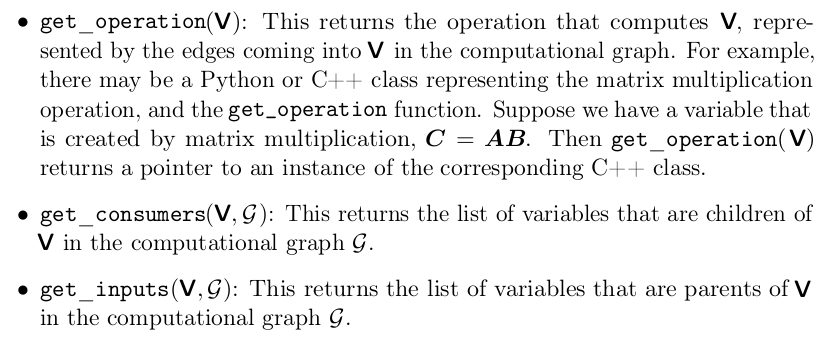
\includegraphics[width=.9\linewidth]{Deep Feedforward Networks/screenshot_2018-10-02_08-51-44.png}
\end{center} 

\begin{itemize}
\item Each operation \texttt{op} is also associated with a \texttt{bprop} operation
\begin{itemize}
\item This \texttt{bprop} operation can compute a Jacobian vector product
\item Formally, \texttt{op.bprop(inputs,X,G)} must return:
\end{itemize}
\end{itemize}
\begin{center}
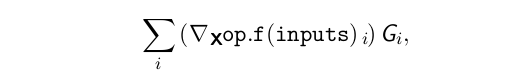
\includegraphics[width=.9\linewidth]{Deep Feedforward Networks/screenshot_2018-10-02_08-58-55.png}
\end{center}
\begin{itemize}
\item Inputs is a list of inputs that are supplied to the operation
\item \texttt{op.f} is the mathematical function that the operation implements
\item \(\mathbf{\mathsf X}\) is the input whose gradient we which to compute
\item \(\mathbf{\mathsf G}\) is the gradient on the output of the operation
\end{itemize}

\begin{center}
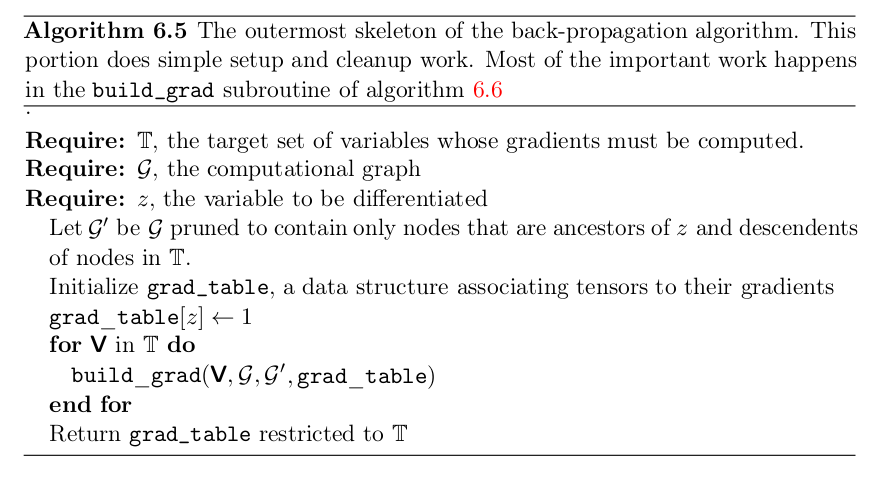
\includegraphics[width=.9\linewidth]{Deep Feedforward Networks/screenshot_2018-10-02_09-04-05.png}
\end{center}

\begin{center}
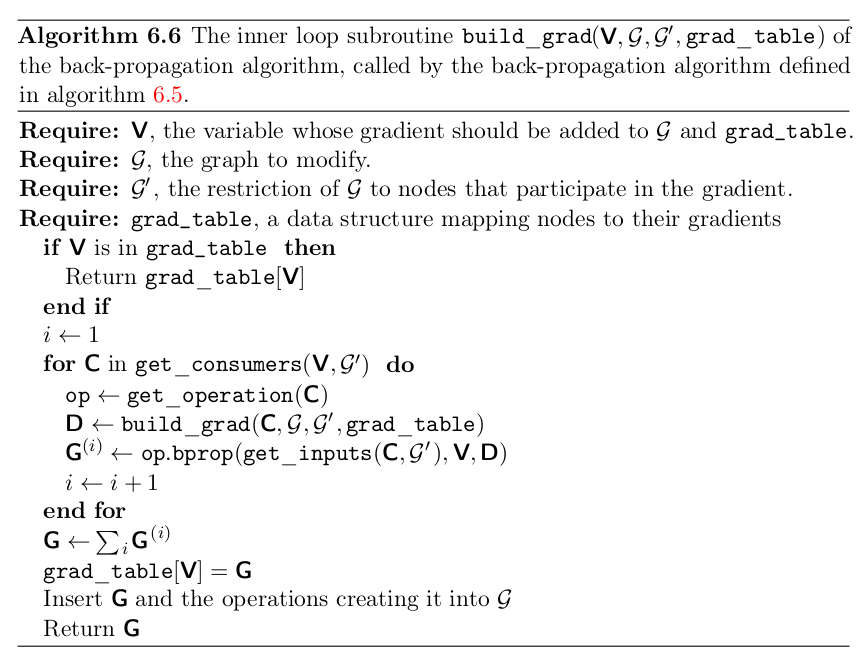
\includegraphics[width=.9\linewidth]{Deep Feedforward Networks/screenshot_2018-10-02_09-04-43.png}
\end{center}

\begin{itemize}
\item The backprop algorithm uses dynamic programming to get a better running time
\end{itemize}

\subsection{Backpropagation equations}
\label{sec:orgfe6d5ad}
\begin{itemize}
\item \(w_{ji}^l\) is the weight from neuron \(i\) in layer \(l-1\) to neuron \(j\) in layer \(l\)
\item \(a_j^1 = x_j\)
\item \(s_j^l=\sum_ia_i^{l-1}w_{j,i}^{l-1}+b_j^{l-1}\)
\item \(a_k^l = \Phi(s_k^l)\)
\item \(\delta_j^l=\frac{\partial e}{\partial s_j^l}\)
\end{itemize}

\begin{center}
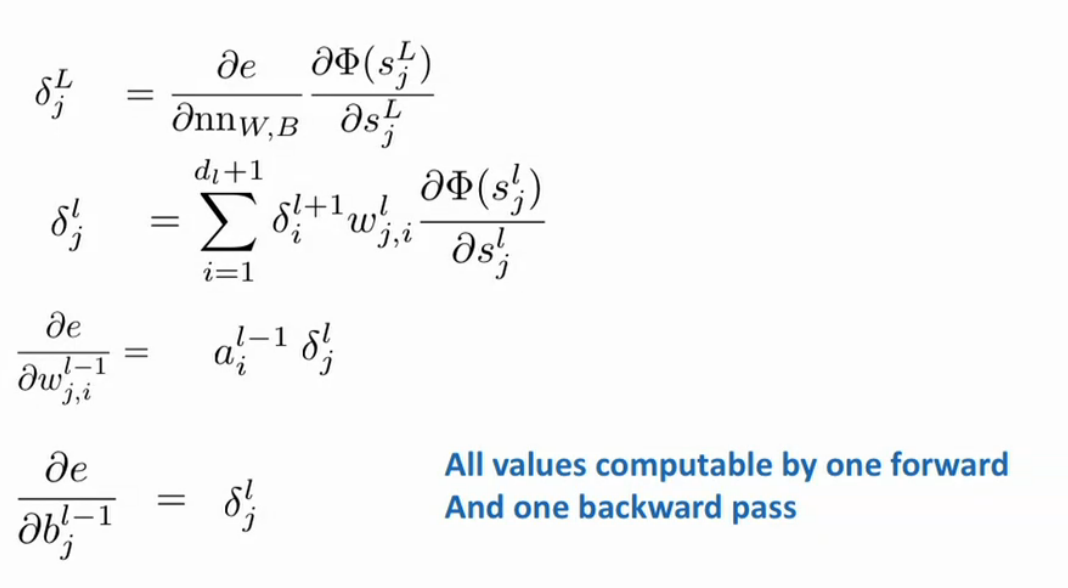
\includegraphics[width=.9\linewidth]{Deep Feedforward Networks/Screenshot-20181009083230-1068x588_2018-10-09_08-33-23.png}
\end{center}

\begin{center}
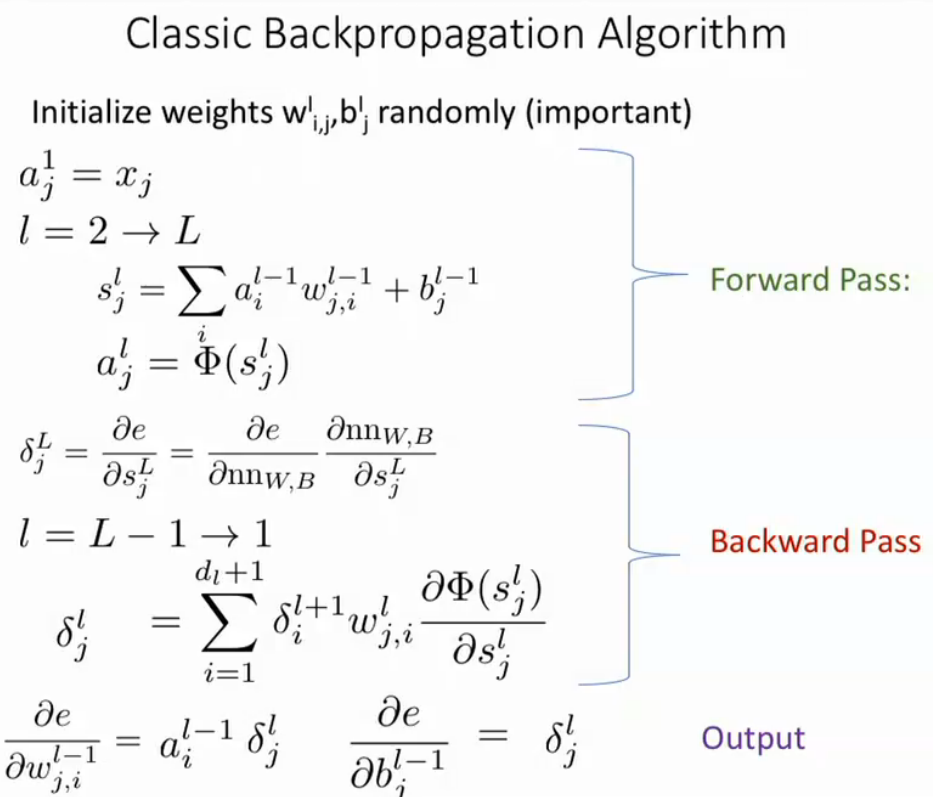
\includegraphics[width=.9\linewidth]{Deep Feedforward Networks/Screenshot-20181009084054-933x797_2018-10-09_08-41-57.png}
\end{center}

\section{Convolutional Networks}
\label{sec:org439882b}
\subsection{General}
\label{sec:orga4b0407}
\begin{itemize}
\item \textbf{Convolutional Networks} (CNNs) are a specialized kind of neural network for processing data that has a grid-like topology
\begin{itemize}
\item \textbf{Convolution} is a specialized kind of linear operation
\item Convolutional networks are neural networks that use convolution in place of general matrix multiplication in at least one of their layers
\end{itemize}
\end{itemize}

\subsection{The Convolution Operation}
\label{sec:orgd31b6e0}
\begin{itemize}
\item A convolution is in its most general form an operation on two functions of a real valued argument
\begin{itemize}
\item Example of a convolution: \(s(t) \int x(a)w(t-a)da\)
\item The convolution operation is typically denoted with an asterisk: \(s(t) = (x*w)(t)\)
\item The first argument to the convolution is often referred to as the \textbf{input}
\item The second argument is referred to as the \textbf{kernel}
\item The output is referred to as the \textbf{feature map}
\item In machine learning applications
\begin{itemize}
\item The input is usually a multidimensional array of data
\item The kernel is usually a multidimensional array of parameters that are adapted by the learning algorithm.
\item The multidimensional dimensional arrays are referred to as tensors
\item Because each element of the input and kernel must be explicitly stored separately, it is often assumed that these functions are zero everywhere but in the finite set of points for which we store the value
\end{itemize}
\item Convolutions are often used over more than one axis at a time
\begin{itemize}
\item e.g. on a two-dimensional image \(I\) as input one would probably use a two dimensional kernel \(K\)
\end{itemize}
\item Convolution is commutative which means that for a two dimensional kernel \(K\) and a input \(I\): \(S(i,j) = (I*K)(i,j)=(K*I)(i,j)\)
\begin{itemize}
\item The last one is usually more straightforward to implement in a machine learning library, since there is less variation in the range of valid values for \(m\) and \(n\)
\end{itemize}
\item Many neural network libraries implement are related function called \textbf{cross-correlation}, which is the same as convolution but without flipping the kernel
\begin{itemize}
\item e.g. \(S(i,j) = (K*I)(i,j)= \sum_m\sum_nI(i+m,j+n)K(m,n)\)
\item Some also call this convolution
\end{itemize}
\end{itemize}
\end{itemize}

\subsection{Motivation}
\label{sec:org8a4dc26}
\begin{itemize}
\item Convolution leverages three important ideas that can help improve a machine learning system:
\begin{itemize}
\item \textbf{Sparse interactions} is accomplished by making the kernel smaller than the input
\begin{itemize}
\item It is also referred to as \textbf{parse connectivity} \textbf{or *sparse weights}
\item e.g. one can detect small meaningful features in images such as edges with kernels
\item One needs to store fewer parameters which reduces the memory requirements of the model and improves its statistical efficiency
\begin{itemize}
\item Computing the output requires fewer operations
\item The improvements in efficiency are usually quite large
\end{itemize}
\end{itemize}

\item \textbf{Parameter sharing:} refers to using the same parameter for more than one function in the model
\begin{itemize}
\item One can say that a network has \textbf{tied weights}, because the value of the weight applied to one input is tied to the value of a weight applied elsewhere
\item Each member of the kernel is used at every position of the input
\end{itemize}

\item \textbf{Equivariant representations}: If \(g\) is any function that translates the input then that is shifts is, then the convolution function is equivalent to \(g\) 
\begin{itemize}
\item A function \(f\) is equivalent to a function \(g\) if \(f(g(x))=g(f(x))\)
\end{itemize}
\end{itemize}

\item Some kinds of data cannot be processed by neural networks defined bymatrix multiplication with a fixed-shape matrix. Convolution enables processing of some of these kinds of data.
\end{itemize}

\subsection{Pooling}
\label{sec:orgc631995}
\begin{center}
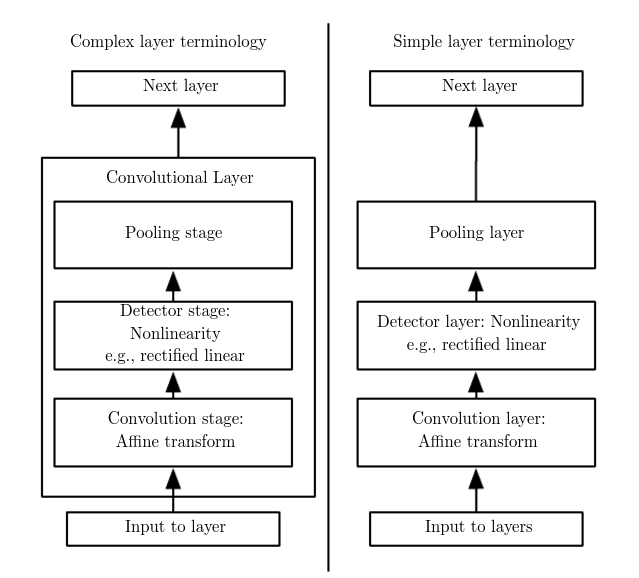
\includegraphics[width=.9\linewidth]{Convolutional Networks/screenshot_2018-10-08_10-23-35.png}
\end{center}

\begin{itemize}
\item A typical layer of a convolutional network consists of three stages
\begin{enumerate}
\item In the first stage the layer performs several convolutions in parallel to produce a set of linear activations
\item In the second stage each linear activation is run through a nonlinear activation, such as rectified linear activation function
\begin{itemize}
\item Is sometimes called the \textbf{detector stage}
\end{itemize}
\item The third stage we use a \textbf{pooling function} to modify the output of the layer further
\begin{itemize}
\item It replaces the output of the net at a certain location with a summary statistic of the nearby output
\begin{itemize}
\item e.g. the \textbf{max pooling operation} which reports the maximum output within a rectangular neighborhood
\end{itemize}
\item Pooling helps to make the representation approximately \textbf{invariant} to small translation of the input
\begin{itemize}
\item Invariance to translation means that if we translate the input by a small amount, the values of most of the pooled outputs
\item Invariance to local translation can be a useful property if we care more about whether some feature is present than exactly where it is.
\end{itemize}
\item It is possible to use fewer pooling units than detector units by reporting summary statistics for pooling regions spaced \(k\) pixels apart rather than \(1\) pixels apart
\begin{itemize}
\item Improves computational efficiency of the network because the next layer has approximately \(k\) times fewer inputs to process
\item Can be used to handle images of variable size by changing how much it is space depending on the input size
\end{itemize}
\end{itemize}
\end{enumerate}
\end{itemize}

\section{Tree-Based Methods}
\label{sec:org960329f}
\subsection{Background}
\label{sec:org46119a7}
\begin{itemize}
\item Three based methods partition the feature space into a set of rectables and then fit a simple model in each one
\begin{itemize}
\item They are simple yet powerful
\item One first split the space into two regions and models the response by the mean of \(Y\) in each region, then one or both of the regions are split into two more regions, this process is continued until some stopping rule is applied
\end{itemize}
\end{itemize}

\subsection{Regression Trees}
\label{sec:orgba60c1d}
\begin{itemize}
\item The data consists of \(p\) inputs and a response, for each of \(N\) observations, that is \((x_i,y_i)\) for \(i=1,2,\dots,N\), with \(x_i=(x_{i1}, x_{i2}, \dots, x_{ip})\)
\item The algorithm needs to automatically decide on the splitting variables and split points and what topology (shape) the three should have
\item If one have a partition into \(M\) regions \(R_1,R_2,\dots,R_M\), and model the response as a constant \(c_m\) in each region:
\end{itemize}
\begin{equation}
  f(x) = \sum_{m=1}^Mc_mI(x \in R_m)
\end{equation}
\begin{itemize}
\item If the criterion is minimization of the sum of squares \(\sum(y_i-f(x_i))^2\), he best \(\hat c_m\) is just the average of \(y_i\) in the region \(R_m\):
\end{itemize}
\begin{equation}
  \hat c_m = \text{ave}(y_i \mid x_i \in R_m ).
\end{equation}
\begin{itemize}
\item Since the binary partition in terms of minimum sum of squares is generally computationally infeasible one needs a greedy algorithm:
\end{itemize}
\begin{center}
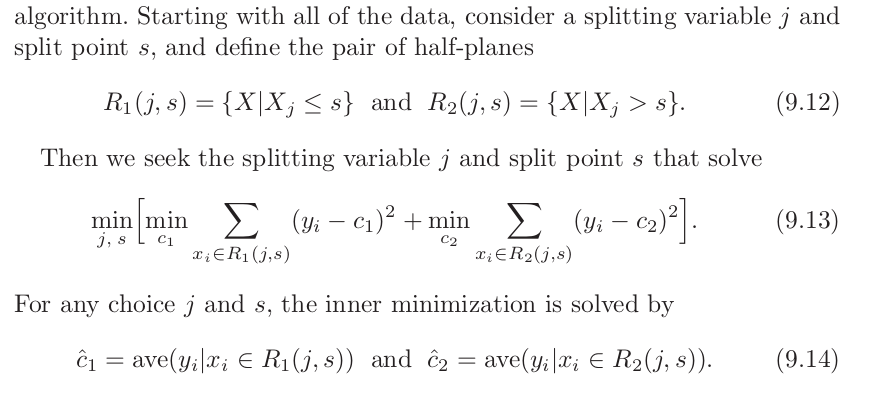
\includegraphics[width=.9\linewidth]{Tree-Based Methods/screenshot_2018-10-08_16-15-20.png}
\end{center}
\begin{itemize}
\item For each splitting variable, the determination of the split point \(s\) can be done very quickly by scanning through all the inputs
\begin{itemize}
\item Having found the best split, one partition the data into the two resulting regions and repeat the splitting process on each of the two regions, which is the repeat on all the resulting regions
\item The optimal tree size should be adaptively chosen from the data
\begin{itemize}
\item A preferred strategy is to grow a large \(T_0\) stopping the splitting process only when some minimum node size is reached
\item The large tree is then pruned using cost-complexity pruning
\end{itemize}
\end{itemize}

\item A \textbf{subtree} \(T \subset T_0\) is defined to be any tree that can be obtained by \textbf{pruning} \(T_0\)
\begin{itemize}
\item Pruning is collapsing any number of its internal (non-terminal nodes).
\item Terminal nodes is indexed by \(m\), with node \(m\) representing region \(R_m\)
\item \(|T|\) denotes the number of terminal nodes in \(T\)
\end{itemize}
\item Letting
\end{itemize}
\begin{center}
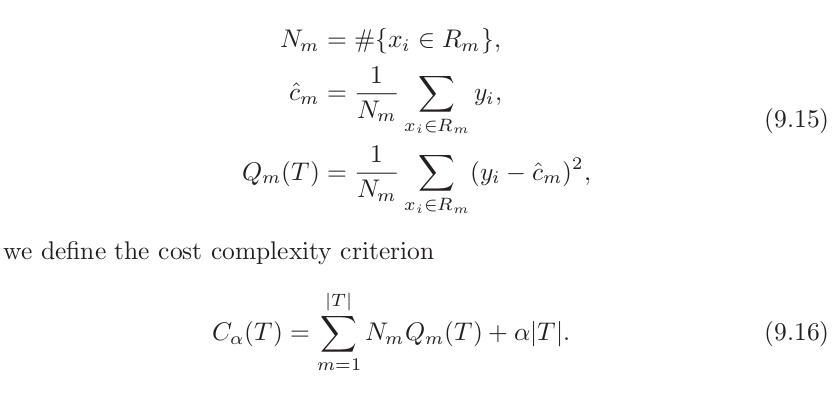
\includegraphics[width=.9\linewidth]{Tree-Based Methods/screenshot_2018-10-08_16-27-26.png}
\end{center}
\begin{itemize}
\item The idea is to find for each \(\alpha\) the subtree \(T_\alpha \subseteq T_0\) to minimize \(C_\alpha(T)\)
\begin{itemize}
\item The tuning parameter \(\alpha \geq 0\) governs the tradeof between tree size and its goodness of fit to the data
\item Larger values of \(\alpha\) result in smaller trees \(T_\alpha\) and the converse for smaller values of \(\alpha\)
\item With \(\alpha = 0\) the solution is the full tree \(T_0\)
\item For each \(\alpha\) there is a unique smallest subtree \(T_\alpha\) that minimizes \(C_\alpha(T)\)
\end{itemize}

\item If one want to find \(T_\alpha\) one uses \textbf{weakest link pruning}:
\begin{itemize}
\item One successively collapse the internal node that produces the smallest per-node increase in \(\sum_m N_mQ_m(T)\) until we produce P and continue until we produce the single-node (root) tree.
\item This gives a finite sequence of subtrees and \(T_\alpha\) must be one of these subtrees
\item Estimation of \(\alpha\) is achieved by five-fold or ten-fold cross-validation:
\begin{itemize}
\item The value \(\hat \alpha\) is chosen to minimize the cross-validated sum of squares
\item The final tree is \(T_{\hat \alpha}\)
\end{itemize}
\end{itemize}
\end{itemize}

\subsection{Classification Trees}
\label{sec:orga0f632e}
\begin{center}
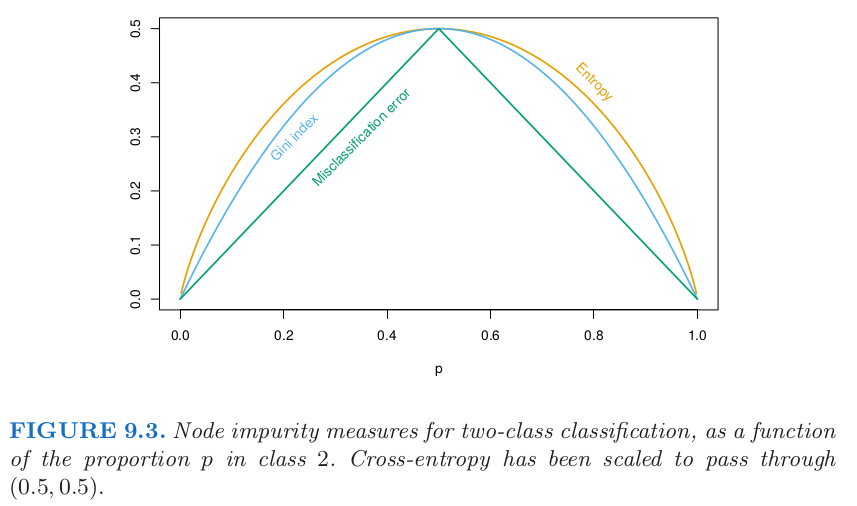
\includegraphics[width=.9\linewidth]{Tree-Based Methods/screenshot_2018-10-08_16-49-37.png}
\end{center}


\begin{itemize}
\item If the target is classification outcome taking values \(1,2,\dots, K\) the only changes needed is the tree algorithm is the criteria for splitting nodes and pruning the tree
\begin{itemize}
\item In a nodes \(m\), representing a region \(R_m\) with \(N_m\) observations, let
\end{itemize}
\end{itemize}
\begin{center}
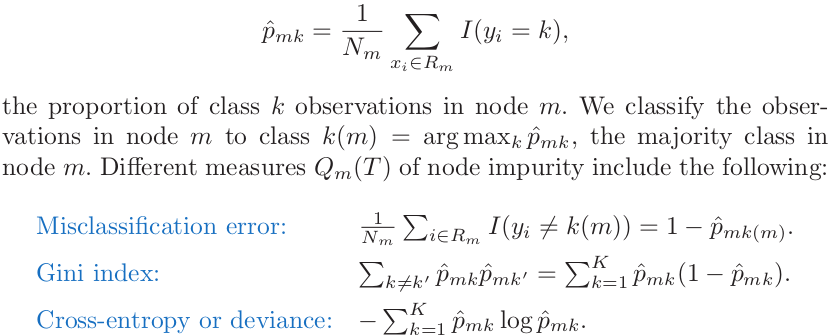
\includegraphics[width=.9\linewidth]{Tree-Based Methods/screenshot_2018-10-08_16-47-14.png}
\end{center}
\begin{itemize}
\item The Gini index and cross-entropy are differentiable and are therefore more amenable to numerical optimization
\begin{itemize}
\item They are often used for growing the three
\item To guide the cost-complexity pruning any of the three measures can be used but typically it is the misclassification rate
\end{itemize}
\end{itemize}

\subsection{Other Issues}
\label{sec:org6249aa2}
\begin{itemize}
\item \textbf{Categorial Predictors}
\begin{itemize}
\item When splitting a predictor having \(q\) possible unordered values, there are \(2^{q-1}-1\) possible partitions of the \(q\) values into two groups
\begin{itemize}
\item The computations become prohibitive for large \(q\)
\end{itemize}
\item With a \(0-1\)  outcome the computation simplifies
\begin{itemize}
\item One orders the predictor classes according to the proportion falling in outcome class \(1\)
\item This gives the optimal split in terms of cross-entropy or Gini index- among all possible \(2^{q-1}-1\) splits
\end{itemize}
\end{itemize}

\item \textbf{The Loss Matrix}: A \(KxK\) loss matrix \(\pmb L\), is defined with \(L_{kk'}\) being the loss incurred for classifying a class \(k\) observation as class \(k'\)
\begin{itemize}
\item Typically no loss is incurred for correct classifications, that is \(L_{kk}= 0 \ \forall k\)
\item To incorporate P the losses into the modeling process, one could modify the Gini index to \(\sum_{k\ne k'} L_{kk'} \hat p_{mk} \hat p_{mk'}\)
\item This does not help in the two-class case and a better approch is to weight the observations in class \(k\) by \(L_{kk'}\)
\end{itemize}

\item \textbf{Missing Predictor Values:} If some of the data has some missing predictor values in some of the values
\begin{itemize}
\item There are two better approaches than throwing the data away
\begin{enumerate}
\item The first is applicable to variable predictors, where one simply makes a new category for \emph{"missing"}
\begin{itemize}
\item This might make one discover that the observation with missing values for some measurement behave differently that those with nonmissing values
\end{itemize}
\item The second is a more general approach which is the construction of surrogate variables
\begin{itemize}
\item When considering a predictor for a split, we use only the observations for which that predictor is not missing
\item Having chosen the best (primary) predictor and split point, we form a list of surrogate predictors and split points.
\begin{itemize}
\item The first surrogate is the predictor and corresponding split point that best mimics the split of the training data achieved by the primary split.
\item The second surrogate is the predictor and corresponding split point that does second best, and so on.
\end{itemize}
\end{itemize}
\end{enumerate}
\end{itemize}

\item \textbf{Why Binary Splits?}
\begin{itemize}
\item The problem with using multiway splits is that it fragment the data too quickly, leaving insufficient data at the next level down.
\item Since multiway splits can be achieved by a series of binary splits, the binary splits are preferred.
\end{itemize}
\end{itemize}

\section{Random forests}
\label{sec:org36cc86c}
\subsection{Introduction}
\label{sec:orgf1d2dba}
\begin{itemize}
\item \textbf{Bagging} or \textbf{bootstrap aggregation} is a technique for reducing the variance of an estimated prediction function
\begin{itemize}
\item Bagging works seems to work especially well for high-variance, low-ias procedures such as trees
\item For regression we simply fit the same regression tree many time to bootstrapsampled versions of the training data and average the result
\item For classification, a \textbf{committee} of trees each cast a vote for the predicted class
\end{itemize}

\item \textbf{Random forests} is a substantial modification of bagging that builds a large collection of de-correlated trees and averages them
\begin{itemize}
\item On many problems its performance is very similar to boosting
\item They are simpler to train and tune than the boosting example
\end{itemize}
\end{itemize}

\subsection{Bootstrap aggregating technique}
\label{sec:org60de636}
\begin{itemize}
\item Given a standard training set \(D\) of size \(n\)
\begin{itemize}
\item Bagging generates \(m\) new training set \(D_i\) each of size \(n'\) by sampling from \(D\) uniformly and with replacement
\begin{itemize}
\item This is know as a \textbf{bootstrap} sample
\end{itemize}
\item The \(m\) models are fitted using the bootstrap sample and combine by
\begin{itemize}
\item Averaging the output (for regresion)
\item Voting (for classification)
\end{itemize}
\end{itemize}
\end{itemize}

\subsection{Definition of Random Forests}
\label{sec:org290417b}
\begin{center}
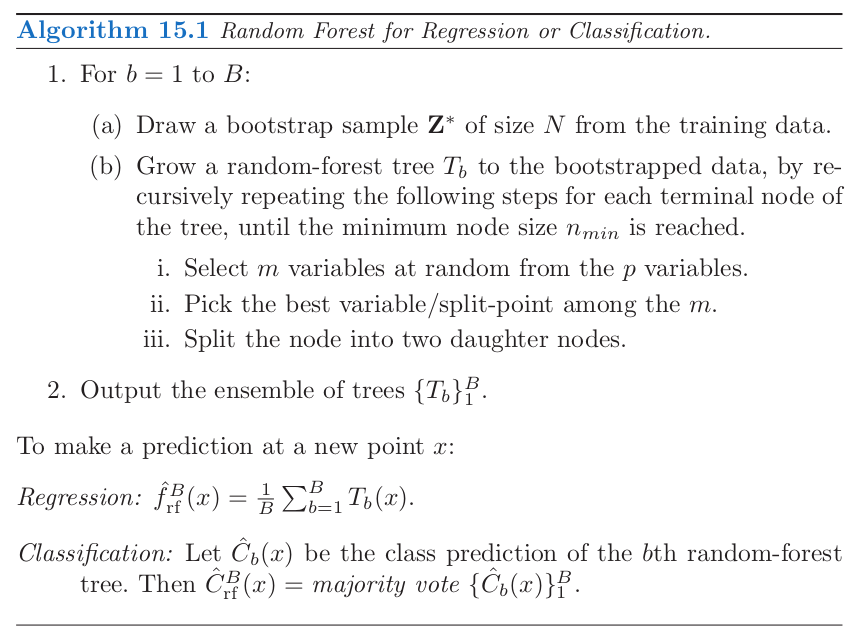
\includegraphics[width=.9\linewidth]{Random forests/screenshot_2018-10-08_20-10-57.png}
\end{center}

\begin{itemize}
\item The essential idea in bagging is to average many noisy but approximately unbiased models
\begin{itemize}
\item This reduces the variance
\item Trees are ideal candidates for bagging since:
\begin{itemize}
\item They can capture complex interaction structures in the data
\item If grown sufficiently deep, they have relative low bias
\end{itemize}
\item Since trees are very noisy they benefit greatly from averaging
\item The bias of bagged trees is the same as that of the individual (bootstrap) trees
\begin{itemize}
\item The only hope of improvement is through variance reduction
\end{itemize}
\end{itemize}

\item An average of \(B\) independent identically distributed random variables, each with variance \(\sigma ^2\) has variance \(\frac1B\sigma^2\)
\begin{itemize}
\item If the variables are simply identically distributed with positive correlation \(\rho\) the variance of the average is
\end{itemize}
\end{itemize}
\begin{equation}
  \rho \sigma^2 + \frac{1-\rho}B \sigma^2
\end{equation}
\begin{itemize}
\item As \(B\) increases, the second terms disappears but the first remains
\begin{itemize}
\item The size of the correlation of pairs of bagged trees limits the benefits of averaging
\item The idea in random forest is to improve the variance reduction of bagging by reducing the correlation between the trees, without increasing the variance to much
\begin{itemize}
\item This is achieved in the tree-growing process through random selection of the input variables
\item Typical values for \(m\) are \(\sqrt p\) or even as low as \(1\)
\item Reducing \(m\) will reduce the correlation between any pair of trees in the ensemble and therefore reduce the variance of the average
\end{itemize}
\item After \(B\) such trees \(\{T(x;\Theta_b)\}^B_1\) are grown the random forest (regression) predictor is
\end{itemize}
\end{itemize}
\begin{equation}
  \hat f_{rf}^B(x) = \frac1B\sum_{b=1}^BT(x;\Theta_b)
\end{equation}
\begin{itemize}
\item Where \(\Theta_b\) characterizes the bth random forest tree in terms of split variables, cutpoints at each nodes, and terminal-node values
\end{itemize}

\begin{center}
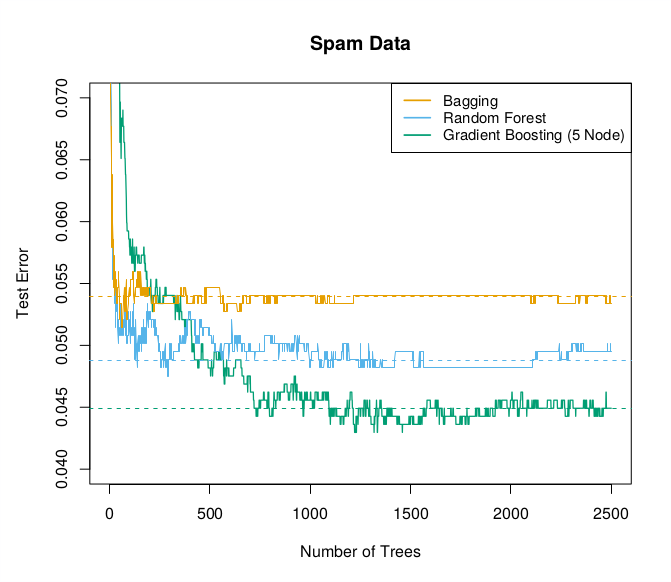
\includegraphics[width=.9\linewidth]{Random forests/screenshot_2018-10-09_08-08-09.png}
\end{center}

\section{Boosting and Additive Trees}
\label{sec:orge24cf66}
\subsection{Boosting Methods}
\label{sec:org3b173b8}
\begin{itemize}
\item The motivation for \textbf{boosting} is to get a procedure that combines the outputs of many "eak" classifiers to produce a powerful "committee"

\item One of the most popular algorithm called AdaBoost.M1 is as follows
\begin{itemize}
\item Consider a two-class problem, with the output variable coded as \(Y \in \{-1,1\}\)
\item Given a vector of predictor variables \(X\), a classifier \(G(X)\) produces a prediction taking one of the two values \(\{-1,1\}\)
\begin{itemize}
\item The error rate on the training sample is
\end{itemize}
\end{itemize}
\end{itemize}
\begin{equation}
  \bar{\text{err}} = \frac1N \sum_{i=1}^N I(y_i \ne G(x_i))
\end{equation}
\begin{itemize}
\item and the expected error on future predictions is \(E_{XY}(I \ne G(X))\)

\item A \textbf{weak classifier} is one whose error rate is only slightly better than random guessing
\begin{enumerate}
\item The purpose of boosting is to sequentially apply the weak classification algorithm to modified versions of the data and produces a sequence of weak classifiers \(G_m(x),m=1,2,\dots,M\)
\item The predictions from all of them are then combined through a weighted majority vote to produce the final prediction
\end{enumerate}
\end{itemize}
\begin{equation}
  G(x) = \text{sign} \bigg( \sum_{m=1}^M \alpha_mG_m(x) \bigg)
\end{equation}
\begin{itemize}
\item \(\alpha_1, \alpha_2, \dots, \alpha_M\) are computed by the boosting algorithm and weight the contribution of each respective \(G_m(x)\)
\begin{itemize}
\item This gives higher influence to the more accurate classifiers in the sequence
\end{itemize}
\end{itemize}

\begin{center}
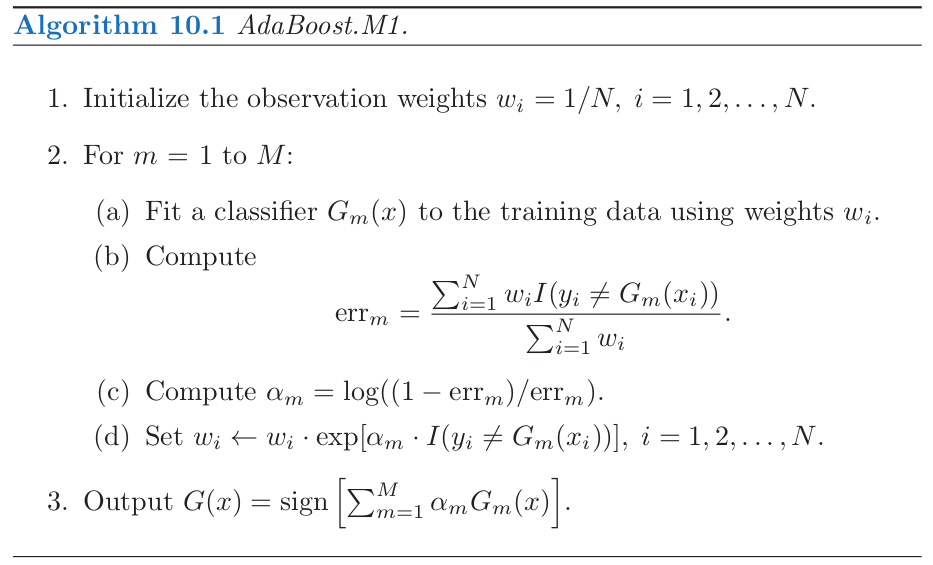
\includegraphics[width=.9\linewidth]{Boosting and Additive Trees/screenshot_2018-10-21_20-24-38.png}
\end{center}

\subsection{Boosting Fits an Additive Model}
\label{sec:org17864b5}
\begin{itemize}
\item The key in boosting \(G(x)\) expression
\begin{itemize}
\item It is a way of fitting an additive expansion in a set of elementary "basiss functions
\item The basis functions are the individual classifiers \(G_m(x) \in \{-1,1\}\)
\item Basis function expansions take the form
\end{itemize}
\end{itemize}
\begin{equation}
	f(x) = \sum_{m=1}^M\beta_mb(x; \gamma_m)
\end{equation}
\begin{itemize}
\item where \(\beta_m\), \(m=1,2,\dots,M\) are the expansion coefficients and \(b(x;\gamma) \in \mathbb R\) are usually simple functions over the multivariate argument \(x\) characterized by a set of parameters \(\gamma\)
\begin{itemize}
\item Typically these models are fit by minimizing a loss function averaged over the training data
\item For many loss functions \(L(y, f(x)\) and/or basis functions \(b(x; \gamma\) this requires computationally intensive numerical optimization techniques
\item A simple alternative can often be found when it is feasible to rapidly solve the subproblem of fitting just a single basis function
\end{itemize}
\end{itemize}
\begin{equation}
	\min_{\beta, \gamma} \sum_{i=1}^NL(y_i,\betab(x_i;\gamma)
\end{equation}

\subsection{Forward Stagewise Additive Modeling}
\label{sec:org51187d8}
\begin{center}
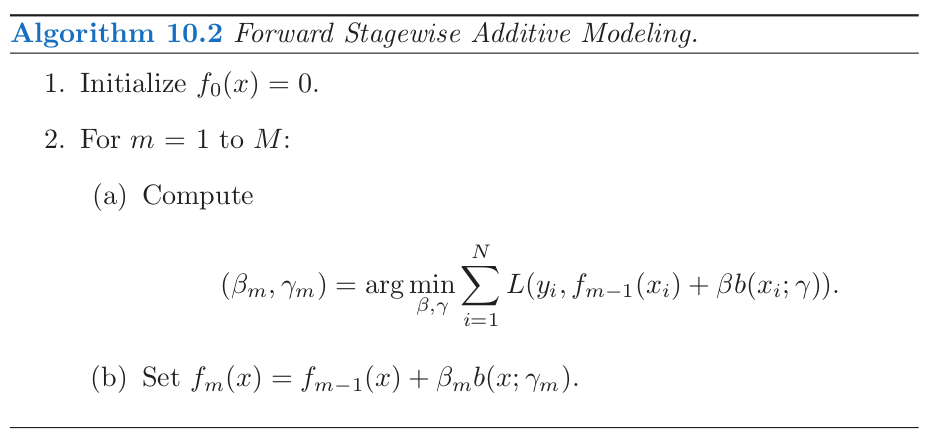
\includegraphics[width=.9\linewidth]{Boosting and Additive Trees/screenshot_2018-10-21_20-44-17.png}
\end{center}

\begin{itemize}
\item \textbf{Forward stagewise modeling} approximates a solution by sequentially adding new basis functions to the expansion without adjusting the parameters and coefficients of those that have already been added 
\begin{itemize}
\item At each iteration \(m\) one solves the optimal basis function \(b(x; \gamma_m)\) and the corresponding coefficient \(\beta_m\) to add to the current expansion \(f_{m-1}(x)\)
\item It produces \(f_m(x)\) and the process is repeated
\end{itemize}

\item For squared loss
\end{itemize}
\begin{equation}
	L(y,f(x)=(y-f(x))^2	
\end{equation}
\begin{itemize}
\item one has
\end{itemize}
\begin{equation}
  \begin{split} 
      L(y_i, f_{m-1}(x_1)+\beta b(x_i;\gamma)) &= (y_i-f_{m-1}(x_i)-\beta b(x_i;\gamma))^2
                                             &= (r_{im}-\beta b(x_i;\gamma))^2
  \end{split}
\end{equation}
\begin{itemize}
\item where \(r_im = y_i - f_{m-1}(x_i)\) is simply the residual (difference) of the current modeland the ith observation
\begin{itemize}
\item Therefore for squared-error loss, the term \(\beta_m b(x;\gamma_m)\) that best fits the current residuals is added to the expansion at each step
\end{itemize}
\end{itemize}

\subsection{Exponential Lost and AdaBoost}
\label{sec:org29ed69c}
\begin{itemize}
\item The \textbf{exponential loss function} is the following
\end{itemize}
\begin{equation}
	L(y,f(X))=\exp(-yf(x))
\end{equation}
\begin{itemize}
\item The exponential loss is more sensitive to changes in the estimated class probabilities

\item AdaBoost.M1 minimizes the exponential loss criterion via a forward-stagewise additive modeling approach
\end{itemize}

\subsection{Why Exponential Loss?}
\label{sec:org8fe7855}
\begin{itemize}
\item The principal attraction of exponential loss in the context of additive modeling is computational
\begin{itemize}
\item It leads to the simple modular reweighting AdaBoost algorithm
\item It has the same population minimizer has binomial log likelihood which is true probabilities
\end{itemize}
\end{itemize}

\subsection{Loss Functions and Robustness}
\label{sec:org9d89341}
\subsubsection{Robust Loss Functions for Classification}
\label{sec:org92f038b}
\begin{figure}[htbp]
\centering
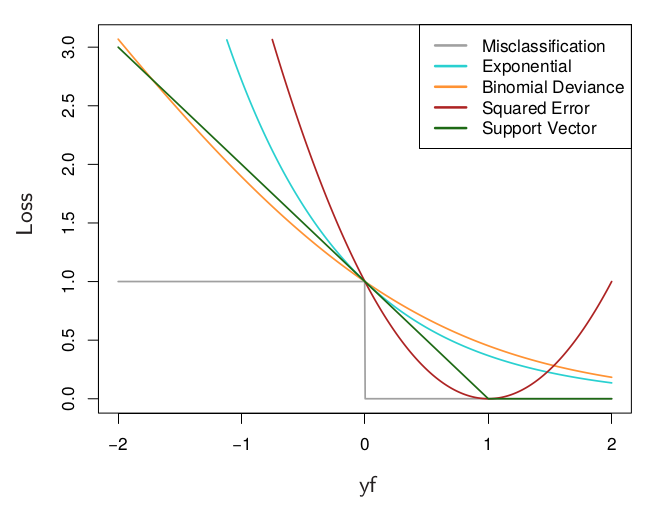
\includegraphics[width=.9\linewidth]{Boosting and Additive Trees/screenshot_2018-10-22_08-47-22.png}
\caption{\label{fig:org3037dfd}
Loss functions for two-class classification}
\end{figure}

\begin{itemize}
\item Since the squared-error is not a decreasing function of the margin it is not good for classification
\begin{itemize}
\item Due to it penalizing large positive correct margins
\end{itemize}

\item For \(K\) classification problems the logistic function generalizes nice
\end{itemize}

\subsubsection{Robust Loss Functions for Regression}
\label{sec:org9cd504b}
\begin{center}
\includegraphics[width=.9\linewidth]{Boosting and Additive Trees/screenshot_2018-10-22_09-19-17.png}
\end{center}

\begin{itemize}
\item In the regression setting, analogous to the relationship between exponential loss and binomial log-likelihood is the relationship between \textbf{squared-error loss} \(L(y,f(x))=(y-f(x))^2\) and \textbf{absolute loss} \(L(y,f(x)) = | y - f(X)|\)
\begin{itemize}
\item The population solutions are
\begin{itemize}
\item For squared-error loss: \(f(x)=  E(Y \mid x)\)
\item For absolute loss: \(\text{median}(Y \mid x)\)
\end{itemize}
\item For symmetric error distributions the two population solutions are the same
\item On finite samples squared-error loss places much more emphasis on observations with large absolutie residual \(|y_i - f(x_i)|\) during the fitting process
\begin{itemize}
\item It is far less robust and it performance severely degrades for the fitting process for long-tailed error distributions and especially for grossly mismeasured y-values ("outliers").
\item Other more robust criteria such as absolute loss perform much better in these situations
\end{itemize}
\end{itemize}

\item A criterion which is much more robust against outliers while being nearly as efficient as least squares is \textbf{Huber loss criterion} used for M-regression
\end{itemize}
\begin{equation}
	L(y,f(x)) = 
		\begin{cases}
			\mbox{$[y-f(x)^2]$} & \mbox{for $|y-f(x)|\leq \delta$} \\
			\mbox{$2\delta| y - f(x) | - \delta^2$} & \mbox{otherwise} \\
		\end{cases}
\end{equation}

\subsection{"Off-the-Shelf" Procedures for Data Mining}
\label{sec:orgedb7c3f}
\begin{center}
\includegraphics[width=.9\linewidth]{Boosting and Additive Trees/screenshot_2018-10-22_09-27-14.png}
\end{center}

\begin{itemize}
\item Of all the well-known learning methods, decision trees come closest to meeting the requirements for serving as an off-the-shelf procedure for data mining
\begin{itemize}
\item They are relatively fast to construct and they produce interpretable models (if the trees are small)
\item They have one aspect that prevents them from being the ideal tool forpredictive learning, namely inaccuracy.
\begin{itemize}
\item They seldom provide predictive accuracy comparable to the best that can be achieved with the data at hand
\end{itemize}
\end{itemize}
\end{itemize}

\subsection{Boosting Trees}
\label{sec:orgb8cc011}
\begin{itemize}
\item A tree can be formally expressed as
\end{itemize}
\begin{equation}
  T(x; \Theta) = \sum_{j=1}^J\gamma_iI(x \in R_j)
\end{equation}
\begin{itemize}
\item with parameters \(\Theta = \{R_j. \gama_j\}_1^J\)
\begin{itemize}
\item \(J\) is usually treated as a meta parameters
\item The parameters are found by minimizing the empirical risk
\end{itemize}
\end{itemize}
\begin{equation}
	\hat \Theta = \arg \min_\Theta \sum_{j=1}^J \sum_{x_i \in R_j} L(y_i, \gamma_j)
\end{equation}	
\begin{itemize}
\item The optimization problem is useful to divide into two parts
\begin{itemize}
\item \textbf{Finding \(\gamma_j\) given \(R_j\)}: \(\hat \gamma = \bar y_j\) is often used and for misclassification \(\hat \gamma\) is the modal class of the observations falling in region \(R_j\)
\item \textbf{Finding \(R_j\)}: It is the difficult part, for which approximate solutions are found
\begin{itemize}
\item Finding \(R_j\) typically involves estimating \(\gamma _j\) as well
\item The typically strategy is to use a greedy, top-down recursive partitioning algorithm to find it
\item It is sometimes necessary to approximate the empirical risk by a smoother and more convenient criterion for optimizing the \(R_j\):
\end{itemize}
\end{itemize}
\end{itemize}
\begin{equation}
	  \tilde \Theta = \arg \min_\Theta \sum_{j=1}^N \tilde L(y_i, T(x_i, \Theta))
\end{equation}	
\begin{itemize}
\item Then given the \(\bar R_j = \tilde R_j\), the \(\gamma\) can be estimated

\item The classification trees described in 9.2 using the \textbf{Gini index} instead of misclassification loss in growing the tree is used in the \textbf{boosted tree model} as a sum
\end{itemize}
\begin{equation}
  f_M(x) = \sum_{m=1}^MT(x; \Theta_m)
\end{equation}
\begin{itemize}
\item induced in a forward stagewise manner
\begin{itemize}
\item At each step in the forward stagewise procedure one must solve
\end{itemize}
\end{itemize}
\begin{equation}
	  \hat \Theta_m = \arg \min_{\Theta_m} \sum_{j=1}^N L(y_i, f_{m-1}(x_i)T(x_i, \Theta_m))
\end{equation}	
\begin{itemize}
\item for the region set and constants \(\Theta_m = \{R_{jm}, \gamma_{jm}\}_1^{J_m}\) of the next tree given the current model \(f_{m-1}(x)\)
\begin{itemize}
\item Given the regions \(R_{jm}\) finding the optimal constants \(\gamma_{jm}\) in each region is typically straightforward:
\end{itemize}
\end{itemize}
\begin{equation}
  \hat \gamma = \arg \min_{\gamma_{jm}} \sum_{x_i \in R_{jm}} L(y_i, f_{m-1}(x_i)+\gamma_{jm})
\end{equation}
\begin{itemize}
\item Finding the regions is difficult, and even more difficult than for a single tree, though for a few special cases it simplifies
\begin{itemize}
\item For squared-error loss, the solution is no harder than for a single tree
\begin{itemize}
\item It is simply the regression tree that best predicts the current residuals \(y_i-f_{m-1}(x_i)\) and \(\hat \gamma _{jm}\) is the mean of these residuals in each corresponding region
\end{itemize}
\item For two-class classification and exponential loss, this stagewise approach gives rise to the AdaBoost method for boosting classification trees
\begin{itemize}
\item If the trees \(T(x; \Theta_m)\) are restricted to be scaled classification trees the the solution is one that minimizes the weighted error rate \(\sum_i=1^N w_i^{(i)} I(y_i \ne T(x_i;\Theta_m))\) with weights \(w_i^{(m)}= e^{-y_if_{m-1}(x_i)}\)
\item A scaled classification tree is \(\beta_mT(x;\Theta_m)\) with the restriction that \(\gamma_{jm} \in \{-1,1\}\)
\item A non-scaled classification three the weighted exponential criterion for the new tree is
\end{itemize}
\end{itemize}
\end{itemize}
\begin{equation}
  \hat \theta_m = \arg \min_{\Theta_m} \sum_{i=1}^N w_i^{(m)} \exp[-y_iT(x_i;\Theta_m)]
\end{equation}
\begin{itemize}
\item It is straightforward to implement a greedy recursive partioning algorithm using this weighted exponential loss as a splitting criterion
\begin{itemize}
\item Given the \(R_{jm}\) one can show that solution is the weighted log-odds in each corresponding region
\end{itemize}
\end{itemize}
\begin{center}
\includegraphics[width=.9\linewidth]{Boosting and Additive Trees/screenshot_2018-10-22_10-28-20.png}
\end{center}

\begin{itemize}
\item Using loss criteria such as the absolute error or the Huber loss in place of squared-error loss for regression, and the deviance in place of exponential loss for classification, will serve to robustify boosting trees
\begin{itemize}
\item Unfortunately, unlike their nonrobust counterparts, these robust criteria do not give rise to simple fast boosting algorithms
\end{itemize}
\end{itemize}

\subsection{Numerical Optimization via Gradient Boosting}
\label{sec:orgfa08dbb}
\subsubsection{General}
\label{sec:org23fed2b}
\begin{itemize}
\item The loss in using \(f(x)\) to predict \(y\) on the training training data is
\end{itemize}
\begin{equation}
  L(f) = \sum_{i=1}^N L(y_i,f(x_i))
\end{equation}
\begin{itemize}
\item The goal is to minimize \(L(f)\) with respect to \(f\)
\begin{itemize}
\item Where \(f(x)\) is constrained to be a sum of trees.
\item Ignoring the constraint, minimizing it can be viewed as a numerical optimization
\end{itemize}
\end{itemize}
\begin{equation}
  \pmb{\hat f} = \arg \min_{\pmb{f}} L(\pmb f) 
\end{equation}
\begin{itemize}
\item where the "parameters \(\pmb f \in \mathbb R ^n\) are the values of the approximating function \(f(x_i)\) for each of the \(N\) data points \(x_i\)
\end{itemize}
\begin{equation}
  \pmb f = \{f(x_1), f(x_2), \dots, f(x_N)\}^T
\end{equation}
\begin{itemize}
\item Numerical optimization procedures solve it as a sum of component vectors
\end{itemize}
\begin{equation}
	\pmb f_M = \sum_{m=0}^M \pmb h_m, \ \pmb h_m \in \mathbb R ^ n
\end{equation}
\begin{itemize}
\item where \(\pmb f_0 = \pmb h_0\) is the initial guess, and each successive \(\pmb f_m\) is based on the current parameters vecor \(\pmb f_{m-1}\) which is the sum of the previously induced updates induced updates.
\begin{itemize}
\item Numerical optimization methods differ in their prescriptions for computing each increment vector \(\pmb h_m\)
\end{itemize}
\end{itemize}

\subsubsection{Steepest Decent}
\label{sec:org4ffc177}
\begin{itemize}
\item Steepest decent chooses \(\pmb h_m = - \rho_m \pmb g_m\) where \(\rho_m\) is a scalar and \(\pmb g_m \in \mathbb R^N\) is the gradient of \(L(\pmb f)\) evaluated at \(\pmb f = \pmb f_{m-1}\)
\begin{itemize}
\item The component of the gradient \(\pmb g_m\) are
\end{itemize}
\end{itemize}
\begin{equation}
  g_{im} = \bigg[\frac{\partial L(y_i, f(x_i))}{\partial f(x_i)}\bigg]_{f(x_i)=f_{m-1}(x_i)}
\end{equation}
\begin{itemize}
\item The step length \(\rho_m\) is the solution to
\end{itemize}
\begin{equation}
  \rho_m = \arg \min_\rho L(\pmb f_{m-1}-\rho \pmb g_m)
\end{equation}
\begin{itemize}
\item The current solution is the updated
\end{itemize}
\begin{equation}
  \pmb f_m = \pmb f_{m-1}-\rho_m\pmb g_m
\end{equation}
\begin{itemize}
\item and the process repeated at the next iteration
\begin{itemize}
\item It can be viewed as a very greedy strategy, since \(\pmb g_m\) is the local direction in \(\mathbb R^N\) for which \(L(\pmb f)\) is most rapidly decreasing
\item 
\end{itemize}
\end{itemize}

\subsubsection{Gradient Boosting}
\label{sec:org0319f7d}
\begin{center}
\includegraphics[width=.9\linewidth]{Boosting and Additive Trees/screenshot_2018-10-22_21-24-34.png}
\end{center}

\begin{itemize}
\item Forward stagewise boosting is a very greedy strategy
\begin{itemize}
\item The tree prediction \(T(x_i;\Theta_m)\) are analogous to the components of the negative gradient
\begin{itemize}
\item The difference between them are that the tree components \(\pmb t_m = \{T(x_1; \Theta_m), \dots T(x_N; \Theta_m)\}\) are not independent
\item They are constrained to the predictions of a \(J_m\) terminal node whereas the negative gradient is the unconstrained maximal descent direction
\item A way to solve this is to induce a tree \(T(x;\Theta_m)\) at the mth iteration whose predictions \(\pmb t_m\) are as close as possible to the negative gradient which leads to
\end{itemize}
\end{itemize}
\end{itemize}
\begin{equation}
    \tilde \theta_m = \arg \min_\theta \sum_{i=1}^N (-g_{im}-T(x_i;\theta))^2
\end{equation}
\begin{itemize}
\item One fits the tree \(T\) to the negative gradient values by least squares
\begin{itemize}
\item Eventough the solution regions \(\tilde R_{jm}\) to this will not be the same as the solution regions to the general loss function, it will be similar enough to server the same purpose
\end{itemize}
\end{itemize}

\subsubsection{Implementations of Gradient Boosting}
\label{sec:orgfc55a89}
\begin{center}
\includegraphics[width=.9\linewidth]{Boosting and Additive Trees/screenshot_2018-10-22_21-27-02.png}
\end{center}
\begin{itemize}
\item The algorithm for classification is similar
\begin{itemize}
\item Lines 2(a)-(d) are repeated \(K\) times at each iteration \(m\), once for each class using 10.38
\item The result at line 3 is \(K\) different (coupled) tree expansions \$f\(_{\text{kM}}\)(x), k=1,2,\dots{},K£
\item The result produce probabilities via the softmax function
\end{itemize}
\end{itemize}

\subsection{Right-Sized Trees for Boosting}
\label{sec:orgd5e1a34}
\begin{itemize}
\item Using pruning to decide the size of the tree results in too large trees to begin with
\begin{itemize}
\item The simplest strategy for avoiding this is to restrict all trees to be the same size \(J_m = J \forall m\)
\item At each iteration a \(J\) terminal node regression tree is induced
\item \(J\) becomes a meta-peter of the entire boosting procedure to be adjusted to maximize the estimate performance
\end{itemize}

\item One can get an idea of useful values for \(J\) by considering the properties of the target function
\end{itemize}
\begin{equation}
  \eta = \arg \min_f \E_{XY} L(Y,f(X))
\end{equation}
\begin{itemize}
\item The target function \(\eta(x)\) is the one with minimum prediction risk on future data
\begin{itemize}
\item This is the function we are trying to approximate
\item On important property of \(\eta(X)\) is the degree to which the coordinate variables \(X^T=(X_1,X_2, \dots, X_p)\) interact with each other
\item ANOVA expansions catches the about of interaction between coordinate variables
\end{itemize}
\end{itemize}
\begin{equation}
  \eta(X) = \sum_j \eta_j(X_j) + \sum_{jk} \eta_jk (X_j, X_k) + \sum_{jkl} \eta_jkl (X_j, X_k, X_l) + \dots
\end{equation}
\begin{itemize}
\item The sum is over functions of only a single predictor variable \(X_j\)
\begin{itemize}
\item The particular functions \(n_j(X_j)\) are those that jointly best approximate \(\eta(X)\) under the loss criterion being use
\begin{itemize}
\item They are called the "main effect" of X\(_{\text{j}}\)@
\end{itemize}
\item The second sum over two variable functions are called second-order interactions of each respectable variable pair
\item The third sum over three variable functions are called third-order interactions and so on
\item For many problems in practice are typically dominate by low-order interactions
\begin{itemize}
\item When this is the case, models that produce strong higher-order interaction effect such as large decision trees suffer in accuracy
\end{itemize}
\end{itemize}

\item The interaction level of tree based approximations is limited by the tree size \(J\)
\begin{itemize}
\item No interactions effect of level greater than \(J-1\) are possible
\item Since boosted model are additive in the trees this limits them as well
\item Setting \(J=2\) produces models with on allow models with only main effects
\item Setting \(J=2\) produces models where two variable interaction effects are also allowed and so on
\item Experience so far indicates that \(4 \leq J \leq 8\) works well in the context of boosting, with results being fairly insensitive to particular choices in this range
\end{itemize}
\end{itemize}

\subsection{Regularization}
\label{sec:org9ea3cc8}
\subsubsection{General}
\label{sec:org2ec89e2}
\begin{itemize}
\item The other meta-parameter of gradient boosting is the number of boosting interactions \(M\)
\begin{itemize}
\item Each iteration usually reduces training risk \(L(f_M)\)
\item For large enough \(M\) the risk can be made arbitrarily small
\begin{itemize}
\item This can lead to overfitting
\end{itemize}
\item The optimal number \(M^*\) for minimizing future risk is application dependent
\begin{itemize}
\item A way to estimate \(M\) is to use a validation sample
\end{itemize}
\end{itemize}
\end{itemize}

\subsubsection{Shrinkage}
\label{sec:org043ec24}
\begin{itemize}
\item The simplest implementation of shrinkage in the context of boosting is to scale the contribution of each tree by a factor \(0 < \nu < 1\) when it is added to the current approximation
\begin{itemize}
\item Line 2(d) of algorithm 10.3 is replaced by
\end{itemize}
\end{itemize}
\begin{equation}
  f_m(x) = f_{m-1}(x) + \nu \cdot \sum_{j=1}^J \gamma_{j_m} I(x \in R_{jm})
\end{equation}
\begin{itemize}
\item The parameter \(\nu\) can thought of ass the learning rate of the boosting procedure
\begin{itemize}
\item Smaller values of \(\nu\) results in larger training risk for the same number of iterations \(M\)
\item Both \(\nu\) and \(M\) control prediction risk on the training data
\begin{itemize}
\item They are no independent
\item Smaller values of \(\nu\) lead to larger values of \(M\)
\end{itemize}
\item It has been found that smaller values of \(\nu\) favor better test error
\begin{itemize}
\item The best strategy appears to be to set \(\nu\) to be very small (\(\nu < 0.1\)) and then choose \(M\) by early stopping
\item Yields dramatic improvements for regression and probability estimatio
\end{itemize}
\item The price paid for using \(\nu\) is computation
\begin{itemize}
\item Many iterations are generally computationally feasible
\item Even on larger data sets
\item Due to it operating on small trees with no pruning
\end{itemize}
\end{itemize}
\end{itemize}

\subsubsection{Subsampling}
\label{sec:org3acb5db}
\begin{itemize}
\item With \emph{stochastic gradient boosting}, at each iteration we sample a fraction \(\eta\) of the training observations (without replacement) and grow the next tree using that subsample
\begin{itemize}
\item The rest of the algorithm is identical
\item A typically value for \(\eta\) can be \(\frac12\)
\begin{itemize}
\item For larger \(N\) is can be substantially smaller than \(\frac12\)
\end{itemize}
\item It not only reduces computing time but in many cases it actually produces a more accurate model
\end{itemize}

\item The downside is that we have four parameters to set: \(J,M, \nu\) and \(\eta\)
\begin{itemize}
\item Typically some early explorations determine suitable values for \(J, \nu\) and \(\eta\) leaving \(M\) as the primary parameter
\end{itemize}
\end{itemize}

\subsection{Interpretation}
\label{sec:org6b1b0ca}
\subsubsection{General}
\label{sec:org70c94b2}
\begin{itemize}
\item Single decision trees are highly interpretable.
\begin{itemize}
\item The model can be completely represented by a simple two-dimensional graphic (binary tree) that is easily visualized.
\item Linear combinations of trees (10.28) lose this important feature, and must therefore be interpreted in a different way.
\end{itemize}
\end{itemize}

\subsubsection{Relative Importance of Predictor Variables}
\label{sec:orgd989446}
\begin{itemize}
\item In data mining applications the input predictor variables are seldom equally relevant.
\begin{itemize}
\item Often only a few of them has substantial influence on the response
\begin{itemize}
\item Vast majority are irrelevant
\end{itemize}
\item It is often useful to learn the relative importance or contribution of each variable in an given prediction
\begin{itemize}
\item For a single decision tree \(T\) the following is a measurement of relevance for ech predictor variable \(X_\ell\)
\end{itemize}
\end{itemize}
\end{itemize}
\begin{equation}
  \mathcal{T}^2(T) = \sum_{t=1}^{J-1}\hat i_t^2 I(v(t) = \ell)
\end{equation}  
\begin{itemize}
\item The sum is over the internal nodes of the tree.
\begin{itemize}
\item At each node \(t\) one of the input variables \(X_{v(t)}\) is used to partition the  region associated with that node into two sub regions
\begin{itemize}
\item Within each a separate constant is fit to the response values
\item The particular variable chosen is the once that gives maximal estimate improvement \(\hat i_t^2\) in squared error risk over that for a constant fit over the entire region
\item The squared relative importance of variable \(X_\mathcal L\) is the sum of sub squared improvements over all internal nodes
\end{itemize}
\item This importance is easily generalized to additive tree expansions
\end{itemize}
\end{itemize}
\begin{equation}
  \mathcal T^2_\ell = \frac1M \sum_{m=1}^M\mathcal T^2_\ell (T_m)
\end{equation}
\begin{itemize}
\item This measure is more reliable than for a single tree
\begin{itemize}
\item Both measurements referees to the squared relevance
\end{itemize}
\end{itemize}

\subsubsection{Partial Dependence Plots}
\label{sec:org29e5676}
\begin{itemize}
\item The step after identifying the most relevant variable is to attempt to understand the nature of the dependence of the approximation \(f(X)\) on their join values
\begin{itemize}
\item Graphical renderings of the \(f(X)\) as a functions of its arguments gives a comprehensive summary of this de dependence 
\begin{itemize}
\item Limited to low-dimensional view
\item Can be viewed by fixing all but one or two producing a trellis of plots
\end{itemize}
\end{itemize}

\item A general function \(f(X)\) will in principle depend on all of the input variables: \(f(x)=f(X_\mathcal{S}, X_\mathcal{C})\) 
\begin{itemize}
\item One way to define the average or partial dependence of \(f(X)\) on \(X_\mathcal{S}\) is
\end{itemize}
\end{itemize}
\begin{equation}
  f_{\mathcal S} (X_\mathcal S) = E_{X_c}f(X_\mathcal S,X_\mathcal C)
\end{equation}
\begin{itemize}
\item This can server as a useful description of the effect of the chosen subset on \(f(X)\)
\begin{itemize}
\item e.g. when the variables in \(X_\mathcal S\) do not have strong interactions with those in \(X_\mathcal C\)
\item 
\end{itemize}

\item Partial dependence function can used to interpret the result of any "black box" learning method
\begin{itemize}
\item One way to estimate them is
\end{itemize}
\end{itemize}
\begin{equation}
    \hat f_{\mathcal S} (X_\mathcal S) = \frac1N \sum_{i=1}^Nf(X_\mathcal S,X_{i'\mathcal C})
\end{equation}
\begin{itemize}
\item where \(x_{1\mathcal C}, x_{2\mathcal C}, \dots, x_{N\mathcal C}\) are the values of \(X_\mathcal C\) occurring in the training data
\begin{itemize}
\item It can be rapidly computed from the tree itself without reference to the data
\end{itemize}
\end{itemize}

\section{Sequential Data}
\label{sec:org9329022}
\subsection{Markov Models}
\label{sec:org11c61eb}
\begin{itemize}
\item Without the loss of generality one can use the product rule to express the joint distribution for a sequence of observations in the form
\end{itemize}
\begin{equation}
  p(\pmb x_1, \dots, \pmb x_N) = \prod_{n=1}^N p(\pmb x_n \mid \pmb x_1, \dots, \pmb x_{n-1})
\end{equation}
\begin{itemize}
\item If it is assumed that each of the conditional distributions on the right-hand side is independent of all previous observations except the most recent, we obtain the first-order Markov chain
\begin{itemize}
\item The joint distribution for a sequence of \(N\) observations under this models is given by
\end{itemize}
\end{itemize}
\begin{equation}
  p(\pmb x_1, \dots, \pmb x_N) = p(\pmb x_1) \prod_{n=2}^N p(\pmb x_n \mid \pmb x_{n-1})
\end{equation}
\begin{itemize}
\item The conditional distribution for observation \(\pmb x_n\), given all of the observations up to time \(n\) is this given by
\end{itemize}
\begin{equation}
	p(\pmb x_n \mid \pmb x_1, \dots, \pmb x_{n-1}) = p(\pmb x_n \mid \pmb x_{n-1})
\end{equation}
\begin{itemize}
\item In most applications of these model, the conditional distributions \(p(\pmb x_n \mid \pmb x_{n-1})\) that define the model will be constrained to be equal
\begin{itemize}
\item Known as a \textbf{homogeneous Markov chain}
\item Still very constrained even though it is more general than the independent model
\end{itemize}

\item If predictions also are allowed to depend on the previous-but-one value we obtained a second order Markov chain where the joint distribution know is given by
\end{itemize}
\begin{equation}
	p(\pmb x_1, \dots, \pmb x_N) = p(\pmb x_1) p(\pmb x_2 \mid \pmb x_1) \prod_{n=3}^N p(\pmb x_n \mid \pmb x_{n-1}, \pmb x_{n-2})  
\end{equation}  
\begin{itemize}
\item Each observation is now influenced by two previous observations

\item One can consider extensions to an \(M^\text{th}\)  order Markov chain in which the condition distribution for a particular variable depends on the previous \(M\) variables
\begin{itemize}
\item The price paid for this increased flexibility is that the number of paramers in the models is now much larger
\item The number of parameters is \(K^{M-1}(K-1)\) which grows exponential with \(M\) and is therefore impractical for higher numbers of \(M\)
\end{itemize}

\item For continuous variables we can use linear-Gaussian conditional distributions in which each node has a Gaussian distribution whose mean is a linear function of its parents
\begin{itemize}
\item Known as an autoregressive or AR model
\end{itemize}

\item An alternative approach is to use a parameter model for \(p(x_n \mid x_{n-M}, \dots, x_{n-1})\) such as a neural network
\begin{itemize}
\item Sometime called a tapped delay line
\item The number of parameters can be much smaller than in a completely general model
\item It is achieved at the expense of a restricted family of conditional distributions
\end{itemize}
\end{itemize}


\begin{center}
\includegraphics[width=.9\linewidth]{Sequential Data/screenshot_2018-10-29_11-21-18.png}
\end{center}
\begin{itemize}
\item To build a model for sequences that is not limited by the Markov assumption in any order and that can be specified using a limited number of free parameters
\begin{itemize}
\item It can be achieve by introducing additional latent variables to permit a rich class of models to be constructed out of simple components
\item For each observation \(\pmb x_n\) there is introduced a corresponding latent variable \(\pmb z_n\)
\begin{itemize}
\item May be a different type of dimensionality ti the observed variable
\end{itemize}
\item It is assumed that it is the latent variables that form a Markov chain
\begin{itemize}
\item It gives rice to a graphical structure known as a state space model
\item It satisfies the key conditional independence property that \(\pmb z_{n-1}\) and \(\pmb z_{n+1}\) are independent given \(\pmb z_{n}\) so that
\end{itemize}
\end{itemize}
\end{itemize}
\begin{equation}
  \pmb z_{n+1} \perp\mkern-9.5mu\perp \pmb z_{n-1} \mid \pmb z_n
\end{equation}
\begin{itemize}
\item The joint distribution for this model is given by
\end{itemize}
\begin{center}
\includegraphics[width=.9\linewidth]{Sequential Data/screenshot_2018-10-29_11-18-12.png}
\end{center}
\begin{itemize}
\item There is always a path connecting any two observed variables \(\pmb x_n\) and \(\pmb x_m\) via the latent variables
\begin{itemize}
\item The observation for a given \(\pmb x_{n+1}\) depends on all previous observations
\end{itemize}
\end{itemize}

\subsection{Hidden Markov Models}
\label{sec:orgcab2654}
\subsubsection{General}
\label{sec:org9bc5d66}
\begin{itemize}
\item The hidden Markov model can be viewed as a specific instance of the state space model where the latent variables are discrete 
\begin{itemize}
\item If one examines a single time slice in the model it corresponds to a mixture distribution with component densities given by \(p(\pmb x \mid \pmb z)\)
\item In the case of a standard mixture model the latent variables are discrete multinomial variables \(\pmb z_n\) describing which component of the mixture is responsible or generating the corresponding observation \(\pmb x_n\)
\begin{itemize}
\item It is convenient to use a 1 of \(K\) coding scheme
\end{itemize}
\item The probability distribution of \(\pmb z_n\) is allowed to depend on the state of the previous latent variable \(\pmb z_{n-1}\) through a conditional distribution \(p(\pmb{z}_n | \pmb{z}_{n-1})\)
\begin{itemize}
\item Since they are \(K\) dimensional binary variable, the conditional distribution corresponds to a table of numbers that we denote by \(\pmb A\)
\begin{itemize}
\item Its elements are known as \textbf{transition probabilities}
\item They are given by \(A_{jk} = p(z_{nk} = 1 \mid z_{n-1},j)\)
\item Since they are probabilities they satisfy \(0 \leq A_{jk}} \leq 1\) with \(\sum_k A_{jk} = 1\)
\item It has \(K(K-1)\) independent parameters
\item The conditional distribution can be written explicitly in the form
\end{itemize}
\end{itemize}
\end{itemize}
\end{itemize}
\begin{equation}
  p(\pmb z_n \mid \pmb z_{n-1, \pmb A}) = \prod_{k=1}^K \prod_{j=1}^K A_{jk}^{z_{n-1},jz_{nk}}
\end{equation}
\begin{itemize}
\item The initial latent node \(z_1\) is special in that it does not have a parent node
\begin{itemize}
\item It has a marginal distribution \(p(\pmb z_1)\) represented by a vector of probabilities \(\pmb \pi\) with elements \(\pi \equiv p(z_{z1k}=1)\) so that
\end{itemize}
\end{itemize}
\begin{equation}
  p(\pmb z_1 \mid \pmb \pi) = \prod_{k=1}^K \pi_k^{z_{1k}}
\end{equation}
where \(\sum_k \pi_k = 1\) 

\begin{itemize}
\item The transition matrix is sometimes illustrated diagrammatically by drawing the state as nodes in a state transition diagram e.g.
\end{itemize}
\begin{center}
\includegraphics[width=.9\linewidth]{Sequential Data/screenshot_2018-10-29_16-41-00.png}
\end{center}

\begin{itemize}
\item It is sometimes to take a state diagram and unfold over time
\begin{itemize}
\item This gives an alternative representation known as a \emph{lattice} or \emph{trellis} diagram
\item e.g.
\end{itemize}
\end{itemize}
\begin{center}
\includegraphics[width=.9\linewidth]{Sequential Data/screenshot_2018-10-29_16-43-52.png}
\end{center}

\begin{itemize}
\item The specification of the probabilistic model is completed by defining the conditional distributions of the observed variables \(p(\pmb x_n \mid \pmb z_n, \phi)\), where \(\phi\) is a set of parameter governing the distribution
\begin{itemize}
\item These are known as \textbf{emission probabilities}
\item They might e.g. be given by Gaussians if the elements of \(\pmb x\) are continuous variables or by conditional probability tables if \(\pmb x\) is discrete
\item Since \(\pmb x_n\) is observed the distribution \(p(\pmb x_n, \pmb z_n, \phi)\) consists for a given value of \(\phi\) of a vector of \(K\) numbers corresponding to the \(K\) possible states of the binary vector \(\pmb z_n\)
\item The emission probabilities can be represented in the form
\end{itemize}
\end{itemize}
\begin{equation}
  p(\pmb x_n \mid \pmb z_n, \phi) = \prod_{k=1}^K p(\pmb x_n \mid \phi_k)^{z_{nk}}
\end{equation}

\begin{itemize}
\item The joint probability distribution for a \emph{homogeneous} model over both latent and observed variables is given by
\end{itemize}
\begin{center}
\includegraphics[width=.9\linewidth]{Sequential Data/screenshot_2018-10-29_16-55-53.png}
\end{center}
\begin{itemize}
\item where \(\pmb X = \{x_1, \dots, x_N\}, \pmb Z = \{z_1, \dots, \pmb z_N\}\), and \(\theta = \{\pmb \pi, \pmb A, \phi \}\) denoted the set of parameter governing the model

\item It is generated the following way
\begin{enumerate}
\item We first choose the initial latent variable \(\pmb z_1\) with probabilities govern by the parameters \(\pi_k\)
\begin{itemize}
\item We then sample the corresponding observation \(\pmb x_1\)
\end{itemize}
\item We chose the state of the variable \(\pmb z_2\) according to the transition probabilities \(p(\pmb z_2 \mid \pmb z_1)\) using the already instantiated value of \(\pmb z_1\)
\item If the sample for \(\pmb z_1\) corresponds to state \(j\), then we chose state \(k\) of \(\pmb z_2\) with probabilities \(A_{jk}\) for \(k=1,\dots K\)
\item Once we know \(\pmb z_2\) we can draw a sample for \(\pmb x_2\) and the next latent variable \(\pmb z_3\) and so on
\end{enumerate}

\item If the model has large transition elements \(A_{kk}\) that are much larger than the off-diagonal elements a typical data sequence will have long runs of points generated from a single component

\item There are many variants of the standard HMM model
\begin{itemize}
\item It can e.g. be obtained for instance by putting constraints on the form of the transition matrix \(\pmb A\)
\item An example if the \emph{right-to-left} HMM, which is obtained by setting the elements \(A_{jk}\) of \(\pmb A\) to zero if \(k<j\) 
\begin{itemize}
\item Such models has typically their initial states probabilities for \(p(\pmb z_1)\) modified such that \$p(z\(_{\text{11}}\) = 1) and \(p(z_{1j}) = 0\) for \(j \ne 1\)
\item The state is typically constrained to start in state 1
\item It can also be further constrained to ensure that large changes in the state index do not occur, so that \(A_{jk} = 0\) if \(k>k+ \Delta\)
\end{itemize}
\end{itemize}
\end{itemize}

\subsubsection{Decodings}
\label{sec:org094dfc6}
\begin{itemize}
\item \textbf{Posterior decoding}: \(\pmb z^*_n\) is the most likely state to be in the n'th step
\end{itemize}
\begin{equation}
  \pmb z^*_n = \arg \max_{\pmb z_n} p(\pmb z_n \mid \pmb x_1, \dots, \pmb x_N)
\end{equation}

\subsubsection{Problems}
\label{sec:org8e16298}
\begin{itemize}
\item \textbf{Evaluation problem}
\begin{itemize}
\item What is the probability that a particular sequence of symbols is produced by a particular model
\item Two algorithms are used  (DO NOT confuse them with the forward-backward algorithm).
\begin{enumerate}
\item The forward algorithm
\item The backwards algorithm
\end{enumerate}
\end{itemize}

\item \textbf{Decoding problem}
\begin{itemize}
\item Given a sequence of symbols (your observations) and a model, what is the most likely sequence of states that produced the sequence.
\item For decoding we use the Viterbi algorithm.
\end{itemize}

\item \textbf{Training problem}
\begin{itemize}
\item Given a model structure and a set of sequences, find the model that best fits the data.
\begin{itemize}
\item Can be solved by the following 3 algorithms:
\begin{itemize}
\item MLE (maximum likelihood estimation)
\item Viterbi training(DO NOT confuse with Viterbi decoding)
\item Baum Welch = forward-backward algorithm
\end{itemize}
\end{itemize}
\end{itemize}
\end{itemize}

\subsubsection{Maximum likelihood for the HMM}
\label{sec:org84755cc}
\begin{itemize}
\item If one have observed a data set \(\pmb X = \{\pmb x_1, \dots, \pmb x_N\}\) one can determine the parameters of an HMM using maximum likelihood
\begin{itemize}
\item It can be obtained from the joint distribution by marginalizing over the latent variables
\end{itemize}
\end{itemize}
\begin{equation}
  p(\pmb X \mid \pmb \theta) = \sum_{\pmb Z} p(\pmb X, \pmb Z, \mid \pmb \theta)
\end{equation}
\begin{itemize}
\item Since it does not factorize over \(n\) one cannot simply treat each of the summations over \(\pmb z_n\) independently
\begin{itemize}
\item The summations cannot be performed explicitly because there are \(N\) variables to be summed over each of which has \(K\) states resulting in \(K^N\) terms
\item A further difficulty with this expression is that, because it corresponds to a generalization of a mixture distribution, it represents a summation over the emission models for different settings of the latent variables.
\begin{itemize}
\item Directly maximizing over this will therefore lead to complex expressions with no closed form solutions
\end{itemize}
\end{itemize}

\item The \textbf{EM algorithm} is used to find an efficient framework for maximizing the likelihood function in hidden Markov models
\begin{itemize}
\item It starts with some initial selection for the model parameters which is denoted \(\pmb \theta^\text{old}\)
\item In the E step the parameter values are taken to find the posterior distribution of the latent variables \(p(\pmb Z \mid \pmb X, \pmb \theta^\text{old})\)
\item It then uses this to evaluate the expectation of the logarithm of the complete-data likelihood function, as a function of the parameters \(\theta\), to give the function \(Q(\pmb \theta, \pmb \theta^\text{old})\) defined by
\end{itemize}
\end{itemize}
\begin{equation}
  Q(\pmb \theta, \pmb \theta^\text{old}) = \sum_{\pmb Z} p(\pmb Z \mid \pmb X, \theta^\text{old}) \ln p(\pmb X, \pmb Z \mid \pmb \theta)
\end{equation}
\begin{itemize}
\item \(\gamma(\pmb z_n)\) is used to denote the marginal posterior distribution of a latent variable \(\pmb z_n\) and \(\xi(\pmb z_{n-1}, \pmb z_n)\) to denote the joint posterior distributions of two successive latent variables so that
\end{itemize}
\begin{equation}
  \begin{split} 
    \gamma (\pmb z_n) &= p(\pmb z_n \mid \pmb X, \pmb \theta^\text{old})\\
    \xi (\pmb z_{n-1},\pmb z_n) &= p(\pmb z_{n-1},\pmb z_n \mid \pmb X, \pmb \theta^\text{old})
  \end{split}
\end{equation}
\begin{itemize}
\item For each value of \(n\)
\begin{itemize}
\item We can store \(\gamma(\pmb z_n)\) using a set of \(K\) non-negative number that sum to unity
\item We can store \(\xi (\pmb z_{n-1},\pmb z_n)\) using a \(K \times K\) matrix of non-negative numbers that sum to unit
\end{itemize}
\item \(\gamma (z_{nk})\) is used tot denote the condition probability of \(z_{nk}=1\)
\begin{itemize}
\item A similar notions is used for \(\xi (z_{n-1,j},z_{nk})\)
\end{itemize}
\item Since the expectation of binary random variables is just the probability that it takes the value \(1\) we have
\end{itemize}
\begin{equation}
  \begin{split} 
    \gamma (z_n) &= \mathbb E[z_{nk}] = \sum_{\pmb z} \gamma(\pmb z) z_{nk} \\
    $\xi (z_{n-1,j},z_{nk})$ &= \mathbb E[z_{n-1,j}z_{nk}] = \sum_{\pmb z} \gamma(\pmb z) z_{n-1,j}z_{nk} 
  \end{split}
\end{equation}
\begin{itemize}
\item If we make use of the definitions of \(\gamma\) and \(\xi\) we obtain
\end{itemize}
\begin{center}
\includegraphics[width=.9\linewidth]{Sequential Data/screenshot_2018-11-04_09-38-18.png}
\end{center}
\begin{itemize}
\item The goal of the E step is to evaluate the quantities \(\gamma(\pmb z_n)\) and \(\xi(\pmb z_{n-1}, \pmb z_n)\) efficiently

\item In the M step we maximize \(Q(\pmb \theta, \pmb \theta^\text{old})\) with respect to the parameters \(\pmb \theta = \{\pmb \pi, \pmb A, \pmb \phi\}\) the parameters \(\gamma(\pmb z_n)\) and \(\xi(\pmb z_{n-1}, \pmb z_n)\) are treated as constants
\begin{itemize}
\item Maximization with respect to \(\pmbm \pi\) and \(\pmb A\) is easily achieved by using appropriate Lagrange multipliers with the results
\end{itemize}
\end{itemize}
\begin{center}
\includegraphics[width=.9\linewidth]{Sequential Data/screenshot_2018-11-04_09-46-05.png}
\end{center}

\begin{itemize}
\item The EM algorithm must be initialized by choosing starting values for \(\pmb \pi\) and \(\pmb A\)
\begin{itemize}
\item It should respect the summation constraints associated with their probabilistic interpretation
\item Any elements of \(\pmb \pi\) or \(\pmb A\) that are initially will remain zero in subsequent EM update
\item A typical initialization procedure would involve selecting random starting values of the parameters subject to the summation and non-negativity constraints
\item There are no particular modification to the EM results for the left-to-right models beyond choosing initial values for the elements \(A_{jk}\) in which the appropriate elements are set to zero
\end{itemize}

\item To maximize \(Q(\pmb \theta, \pmb \theta^\text{old})\) with respect to \(\phi_k\) it is only the final term in the extended form that depends on \(\phi_k\)
\begin{itemize}
\item It has the same form as the data-dependent term in the corresponding function for a mixture distribution for i.i.d. data
\item We are simply maximizing the weighted log likelihood function for emission density \(p(\pmb x \mid \pmb \phi_k)\) with weights \(\gamma(z_{nk})\)
\item In the case of Gaussian emission densities we have \(p(\pmb x \mid \phi_k) = \mathcal N (\pmb x \mid \pmb \mu_k, \pmb \Sigma_k)\) and the maximization of the function \(Q(\pmb \theta, \pmb \theta^\text{old})\) gives
\end{itemize}
\end{itemize}
\begin{center}
\includegraphics[width=.9\linewidth]{Sequential Data/screenshot_2018-11-04_09-58-10.png}
\end{center}

\begin{itemize}
\item For the case of discrete multinomial variables the conditional distribution takes the form
\end{itemize}
\begin{center}
\includegraphics[width=.9\linewidth]{Sequential Data/screenshot_2018-11-04_09-59-08.png}
\end{center}
\begin{itemize}
\item and the corresponding M-step equations are given by
\end{itemize}
\begin{center}
\includegraphics[width=.9\linewidth]{Sequential Data/screenshot_2018-11-04_09-59-28.png}
\end{center}
\begin{itemize}
\item The EM algorithm requires initial values for the parameters of the emission distribution.
\begin{itemize}
\item A way to set these is first to treat the data initially as i.i.d. and fit the emission density by maximum likelihood, and then use the resulting values to initialize the parameters for EM.
\end{itemize}
\end{itemize}

\subsubsection{The forward-backward algorithm}
\label{sec:orgf966f04}
\begin{itemize}
\item The \textbf{alpha-beta algorithm} is a variant of the \textbf{forward-backward algorithm}

\item Since the posterior distributions of the latent variables is independent of the form \(p(\pmb x \mid \pmb z)\) all we require is the values of the quantities \(p(\pmb x_n \mid \pmb z_n)\) for each value of \(\pmb z_n\) for every \(n\)
\begin{itemize}
\item Therefore the following conditional independence properties does also hold
\end{itemize}
\end{itemize}
\begin{center}
\includegraphics[width=.9\linewidth]{Sequential Data/screenshot_2018-10-30_09-50-41.png}
\end{center}
\begin{itemize}
\item where \(\pmb X = \{\pmb x_1, \dots, \pmb x_N\}\)

\item To evaluate \(\gamma (z_{nk})\) we can we can use the following formular which uses the Bayers' theorem
\end{itemize}
\begin{equation}
  \gamma (\pmb z_n \mid \pmb X) = \frac{p(\pmb X \mid \pmb z_n)p(\pmb z_n)}{p(\pmb X)}
\end{equation}
\begin{itemize}
\item The denominator \(p(\pmb X)\) is implicitly conditions on the parameter \(\pmb \theta^\text{old}\) of the HMM and there for represents the likelihood function
\begin{itemize}
\item Based on property (13.24) together with the product rule of probability we obtain
\end{itemize}
\end{itemize}
\begin{equation}
  \gamma (\pmb z_n) = \frac{p(\pmb x_1, \dots, \pmb x_n,\pmb z_n)p(\pmb x_{n+1}, \dots, \pmb x_N | \pmb z_n)}{p(\pmb X)} = \frac{\alpha(\pmb z_n)\beta(\pmb z_n)}{p(\pmb X)} 
\end{equation}
\begin{itemize}
\item where the following is defined
\end{itemize}
\begin{equation}
  \begin{split} 
    \alpha (\pmb z_n) &\equiv p(\pmb x_1, \dots, \pmb x_n,\pmb z_n) \\
    \beta (\pmb z_n) &\equiv p(\pmb x_{n+1}, \dots, \pmb x_N \mid \pmb z_n)
  \end{split}
\end{equation}
\begin{itemize}
\item The quantity \(\alpha (\pmb z_n)\) represents the joint probability of observing all of the given data up to time \(n\) and the value of \(\pmb z_n\)
\begin{itemize}
\item \(\alpha(z_{nk})\) is used to denote the value of \(\alpha (\pmb z_n)\) when \(z_{nk}=1\)
\end{itemize}
\item \(\beta (\pmb z_n)\) represents the conditional probability of all future data from time \(n+1\) up to \(N\) given the value of \(\pmb z_n\)

\item To more efficiently compute \(\alpha(\pmb z_n)\) the following equation can be used
\end{itemize}
\begin{equation}
  \alpha(\pmb z_n) = p(\pmb x_n \mid \pmb z_n) \sum_{\pmb z_{n-1}} \alpha (\pmb z_{n-1}) p(\pmb z_n \mid \pmb z_{n-1})
\end{equation}
\begin{itemize}
\item In order to start computing this recursively an initial condition is need which is given by
\end{itemize}
\begin{center}
\includegraphics[width=.9\linewidth]{Sequential Data/screenshot_2018-10-30_10-30-44.png}
\end{center}
\begin{itemize}
\item this tells us that \(\alpha (z_{1k})\), for \(k=1,\dots, K\) takes the value \(\pi_kp(\pmb x_1 \mid \pmb \phi_k)\)
\begin{itemize}
\item To evaluate \(\alpha(\pmb z_n)\) along the chain for every latent node the cost is \(O(K^2N)\)
\end{itemize}

\item Another way to evaluate \(\beta(\pmb z_n)\) is using the following formula
\end{itemize}
\begin{center}
\includegraphics[width=.9\linewidth]{Sequential Data/screenshot_2018-10-30_19-20-42.png}
\end{center}
\begin{itemize}
\item The starting point for recursion is now \(\beta(\pmb z_N)\) which is equal to
\end{itemize}
\begin{equation}
  p(\pmb z_n \mid \pmb X) = \frac{p(\pmb X, \pmb z_n)\beta(\pmb z_n)}{p(\pmb X)}
\end{equation}

\begin{itemize}
\item If we sum both sides over \(\pmb z_n\) and just the fact that the left-hand side is a normalized distribution we obtain
\end{itemize}
\begin{equation}
  p(\pmb X) = \sum_{\pmb z_n} \alpha ( \pmb z_n) \beta (\pmb z_b)
\end{equation}

\(p(\pmb X)\) can be computed by the following formula
\begin{equation}
  p(\pmb X) = \sum_{\pmb z_n} \alpha (\pmb z_N)
\end{equation}
this is much better computing it by summing over all possible values of \(\pmb Z\) 

\begin{itemize}
\item To implement the forward algorithm without numeric problems \(\hat \alpha (\pmb z_n)\) is used
\end{itemize}
\begin{equation}
	\hat \alpha (\pmb z_n) = \frac{\alpha (\pmb z_n)}{\prod_{m=1}^n c_m}
\end{equation}
\begin{itemize}
\item where \(c_n = p (\pmb x_n \mid \pmb x_1, \dots, \pmb x_{n-1})\)

\item To compute the basis step the following formula is used
\end{itemize}
\begin{equation}
  \hat \alpha (\pmb z_1) = \frac{\alpha(\pmb z_1)}{c_1}
\end{equation}
\begin{itemize}
\item where \(c_1 = \sum_{k=1}^{K} \pi_k p(\pmb x_1 \mid \phi_k)\)

\item To compute the recursion step the following formula is used
\end{itemize}
\begin{equation}
  \delta (\pmb z_{n}) = c_n \hat a (\pmb z_{n}) = p(\pmb x_n \mid \pmb z_n) \sum_{\pmb z_{n-1}} \hat \alpha (\pmb z_{n-1}) p(\pmb z_n \mid \pmb z_{n-1})
\end{equation}
\begin{itemize}
\item The \(c_n\) is computed an stored as
\end{itemize}
\begin{equation}
	c_n = \sum_{k=1}^K \delta (z_{zk})
\end{equation}
\begin{itemize}
\item Then compute and store \(\hat \alpha(z_{nk}) = \delta(z_{nk})/c_n\)

\item To implement the backward algorithm without numeric problems \(\hat \beta (\pmb z_n)\) is used
\end{itemize}
\begin{equation}
  \hat \beta = {\beta(\pmb z_b)}{\prod_{m=n+1}^N c_m}
\end{equation}
\begin{itemize}
\item The basis step is \(\hat \beta (\pmb z_N) = 1\) as the unscaled version
\item The recursion step \(n\) is to compute the following \(K\) values \(\epsilon(z_{n1}), \dots, \epsilon(z_{nK})\)
\end{itemize}
\begin{equation}
  \epsilon (\pmb z_n) = c_{n+1} \hat \beta(\pmb z_n) = \sum_{z_{n+1}} \hat \beta (\pmb z_{n+1}) p(\pmb x_{n+1} \mid \pmb z_{n+1}) p(\pmb z+1 \mid \pmb z_n)
\end{equation}
\begin{itemize}
\item Using the \(c_{n+1}\) computed during forward recursion compute and store \(\hat \beta (z_{nk}) = \epsilon (z_{nk}) / c_{n+1}\)

\item Using the scaled versions \(\hat \alpha\) and \(\hat \beta\) the following holds
\end{itemize}
\begin{equation}
  p(\pmb z_n \mid \pmb x_1, \dots, \pmb x_N) = \hat \alpha (\pmb z_n) \hat \beta (\pmb z_n)
\end{equation}

\begin{itemize}
\item Then the posterior decoding \(\pmb z_n^*\) for a given \(n\) becomes
\end{itemize}
\begin{equation}
  \pmb z_n^* = \arg \max_{\pmb z_n} \hat \alpha (\pmb z_n)  \hat \beta (\pmb z_n)
\end{equation}

\subsubsection{The Viterbi decoding}
\label{sec:org1eb51ab}
\begin{itemize}
\item \textbf{Viterbi decoding}: \(Z^*\) is the overall most likely explanation of \(\pmb X\) :
\end{itemize}
\begin{equation}
  \pmb Z^* = \arg\max_{\pmb{z}} p(\pmb X, \pmb Z \mid \pmb \Theta)
\end{equation}

\begin{itemize}
\item The following is true for \(p(\pmb X, \pmb Z^*)\)
\end{itemize}
\begin{equation}
	p(\pmb X, \pmb Z^*) = \max_{\pmb z_N} \omega (\pmb z_N)
\end{equation}
\begin{itemize}
\item where \(\omega (\pmb z_n) \equiv \max_{z_1, \dots, \pmb z_{n-1}} p(\pmb x_1, \dots, \pmb x_n, \pmb z_1 \dots, \pmb z_n)\) is the probabilitry of the most likely sequence of state \(\pmb z_1, \dots, \pmb z_n\) ending in \(\pmb z_n\) generating the observations \(\pmb x_1, \dots, \pmb x_n\)

\item \(\omega\) can be computed recursivly using the following which takes time \(O(K^2N)\) and space \(O(KN)\) using memorization
\begin{itemize}
\item A table where \(\omega[k][n] = \omega(\pmb z_n)\) if \(\pmb z_n\) is state \(k\)
\item Basis: \(\omega (\pmb z_1) = p(\pmb x_1, \pmb z_1) = p(\pmb z_1) p(\pmb x_1 \mid \pmb z_1)\)
\item Recursion step: \(\omega (\pmb z_n) = p(\pmb x_n \mid \pmb z_n) \max_{\pmb z_{z-1}} \omega (\pmb z_{n-1}) p(\pmb z_n \mid \pmb z_{n-1})\)
\end{itemize}

\item To find \(\pmb Z^*\) from the \(\omega\) table one can just do backtrack and find out which probability with the equation
\begin{itemize}
\item It takes \(O(KN)\) and space \(O(KN)\) using \(\omega\)
\end{itemize}
\end{itemize}

\subsubsection{Extension of the hidden Markov model}
\label{sec:orgd99239f}
\begin{itemize}
\item The basic hidden Markov model, along with the standard training algorithm based on maximum likelihood, has been extended in numerous ways to meet the requirements of particular applications

\item If the goal is sequence classification, there can be significant benefit in determining the parameters of hidden Markov models using discriminative rather than maximum likelihood techniques.
\begin{itemize}
\item Suppose we have a training set of \(R\) observation sequences \(X_r\), where \(r=1,\dots, R\) each of which is labelled according to its class \(m\), where \(m=1,\dots, M\)
\item For each class, we have a separate hidden Markov model with its own parameters \(\pmb \theta_m\)
\item The problem of determining the parameter values is done as a standard classification problem where the cross-entropy is optimized
\end{itemize}
\end{itemize}
\begin{equation}
\sum_{r=1}^R \ln p(m_r \mid \pmb X_r)
\end{equation}
\begin{itemize}
\item Using Bayes’ theorem this can be expressed in terms of the sequence probabilities associated with the hidden Markov models
\end{itemize}
\begin{center}
\includegraphics[width=.9\linewidth]{Sequential Data/screenshot_2018-11-11_20-10-55.png}
\end{center}

\begin{itemize}
\item where \(p(m)\) is the prior probability of class \(m\)
\begin{itemize}
\item Optimization of this cost function is more complex than for maximum likelihood
\item It requires that every training sequence be evaluated under each of the models in order to compute the denominator
\end{itemize}

\item A significant weakness of the hidden Markov model is the way in which it represents the distribution of times for which the system remains in a given state
\begin{itemize}
\item The problem is that the probability that the Markov model will spend precisely \(T\) steps in state \(k\) and then make a transition is a exponentially decaying function of \(T\)
\item For many applications, this will be a very unrealistic model of state duration
\item The problem can be resolved by
\begin{itemize}
\item Modelling state duration directly in which the diagonal coefficients \(A_{kk}\) are all set to zero
\item Each state \(k\) is explicitly associated with a probability distribution \(p(T \mid k)\) of possible duration times.
\end{itemize}
\end{itemize}

\item A limitation of the standard HMM is that it is poor at capturing longrange correlations between the observed variables
\begin{itemize}
\item i.e. variables that are separated by many time steps
\item One way to address this is to generalize the HMM to give the autoregressive hidden Markov model
\begin{itemize}
\item For discrete observations it corresponds to expanded tables of conditional probabilities for the emission distributions
\end{itemize}
\end{itemize}
\end{itemize}

\section{Conditional probabilities and graphical models}
\label{sec:orgb468ddd}
\subsection{You have a joint probability — Now what?}
\label{sec:org9633611}
\begin{itemize}
\item We can split a variables into three kinds
\begin{itemize}
\item Those we have observed
\begin{itemize}
\item Which are thus no longer random
\end{itemize}
\item Those we don't care about
\begin{itemize}
\item They are called nuisance parameter
\item They are just there to build the model
\end{itemize}
\item The parameters we are interested in
\begin{itemize}
\item It can be underlying parameters
\item Future events we want to predict
\end{itemize}
\end{itemize}

\item \textbf{Condition on observed parameters}: If we have the joint probability \(p(X,Y,Z)\) but we have already observed \(Z = z\) we are no longer interested in the outcome of \(Z\) any longer
\begin{itemize}
\item We will still be interested in \(X\) and \(Y\)
\item When observing \(Z\) we move our interest from \(p(X,Y,Z)\) to \(p(X,Y \mid Z)\)
\item It can in general be done from marginalization e.g.
\end{itemize}
\end{itemize}
\begin{equation}
  p(X,Y \mid Z) = \frac{p(X,Y,Z)}{p(Z)}
\end{equation}
\begin{itemize}
\item and
\end{itemize}
\begin{equation}
  p(Z) = \sum_X \sum_Y p(X,Y,Z) 
\end{equation}

\begin{itemize}
\item \textbf{Marginalise away nuisance parameters:} If one is only interested in the outcome of \(X\) and the \(Y\) variable that was needed to connect the variable of interest to the variable \(Z\) but in itself has no use
\begin{itemize}
\item The interest does not lie in \(p(X,Y \mid Z)\) but in \(p(X \mid Z)\) which can be obtained from marginalization
\end{itemize}
\end{itemize}
\begin{equation}
  p(X \mid Z) = \sum_Y $p(X,Y \mid Z)$
\end{equation}

\begin{itemize}
\item The summing over all possible values used in the marginalisation is potentially computational intractable, so one cannot always simply do this
\begin{itemize}
\item Some times clever algorithms are necessary, but they will typically always just do one of those two things in a clever way
\end{itemize}
\end{itemize}

\subsection{Dependency graphs}
\label{sec:org8e13902}
\begin{figure}[htbp]
\centering
\includegraphics[width=.9\linewidth]{Sequential Data/screenshot_2018-10-29_18-41-07.png}
\caption{\label{fig:orgd565641}
Dependency Graph Example for the distribution \(p(X_1, X_2, X_3, X_4)\)}
\end{figure}

\begin{itemize}
\item A graphical notation for describing dependency relationships when specifying a joint distribution
\begin{itemize}
\item Each random variable is represented as a node
\item Whenever the composition of the joint probability has a term \(p(Y \mid X, \dots, X_k)\) we have directed edges from all \(X_i\)'s to \(Y\)
\end{itemize}
\end{itemize}

\section{Johnson-Lindenstrauss Dimensionality Reduction}
\label{sec:orgf24fdff}
\subsection{Intro}
\label{sec:org244d90e}
\begin{itemize}
\item The goal of \textbf{dimensionality reduction} is to represent a high dimensional data set in a lower dimensional space while preserving much of the important structure

\item \textbf{Principal Component Analysis} is a well known dimensionality reduction technique that finds (a few) directions of high variance in the data and projects the data onto these vectors of maximal variance
\begin{itemize}
\item The idea is to maintain as much variance in the data as possible (the structure) while reducing the dimensionality
\item The mapping of data from a high dimensional space to a low dimensional space is called an \textbf{embedding}
\begin{itemize}
\item i.e. we embed the higher dimensional data points in the lower dimensional space
\end{itemize}
\item The dimensionality reduction technique described approximately presevers all pairwise distances between the data points.
\end{itemize}

\item A fundamental result of Johnson and Lindenstrauss says that any \(m\) point subset of Euclidean space can be linearly embedded in \(k=O(\lg m/\epsilon^2)\) dimensions without distorting the distances between any pair of points by more than a factor of \(1 \pm \epsilon\) for any \(0 < \epsilon < \frac12\)
\begin{itemize}
\item For Principal Component Analysis to be relevant the original data points \(x_1, \dots, x_m\) must be inherently low dimensional
\item The \textbf{Johnson-Lindenstraus theorem} requires no assumption on the original data and the target dimension is even independent of the input dimension
\item Another fundamental result og Larsen and Nelson, shows that that the Johnson-Lindenstrauss Lemma is tight even for non-linear embedding!
\item Besides the obvious application of using dimensionality for compression, the Johnson–Lindenstrauss theorem has found numerous applications in algorithms and machine learning for instance for Approximate
\end{itemize}
\end{itemize}
k-Means, Linear Regression, and Approximate Nearest Neighbors.

\subsection{Simple JL Lemma}
\label{sec:org80259aa}
\begin{itemize}
\item \textbf{Theorem 1} For any \(0 < \epsilon < \frac12\) and any integer \(m\), then for integer
\end{itemize}
\begin{equation}
  k = O (\frac1{\epsilon^2} \lg m)
\end{equation}
\begin{itemize}
\item large enough and any points \(x_1, \dots, x_m \subset \mathbb R^d\) there exists a linear map (matrix) \(L: \mathbb R^d \to \mathbb R^k\) such that for any \(1 \leq i, j \leq m\)
\end{itemize}
\begin{equation}
	(1- \epsilon) || x_i - x_j ||_2^2 ||L x_i - Lx_j||^2_2 \leq (1+\epsilon) ||x_i - x_j||^2_2
\end{equation}

\begin{itemize}
\item The linear transformation \(L\) in Theorem 1 is simply multiplication by a matrix whose entries are sampled independently from a standard Gaussian
\begin{itemize}
\item To be precise define a random variable \(A\) as a \(k \times d\) matrix where each entry \(A_{i,j} \sim \mathcal N(0,1)\)
\item The final embedding matrix is sample of the random variable \(L= \frac1{\sqrt k} A\)
\end{itemize}

\item \textbf{Lemma 1.} Fix any vector unit vector \(x\). For any \(0 < \epsilon, \delta < \frac12\). For \(k = O(\epsilon ^{-2}\log \frac1\delta)\) large enough let \(L = \frac1{\sqrt k}\) be a random variable where \(A\) is a \(k \times d\) random matrix whose entries are independent zero mean Gaussians (\(\sim \mathcal N(0,1)\)) Then:
\end{itemize}
\begin{equation}
	\Pr_L(|||Lx||^2 - 1| > \epsilon \leq delta
\end{equation}
\begin{itemize}
\item Stated differently, for any unit vector \(x\) and values of \(0 < \epsilon, \delta < \frac12\). If we pick a random matrix as described, then with probability at least \(1- \delta\) the norm of \(x\) is distorted by a vector at most \((1 \pm \epsilon)\) by \(L\)
\begin{itemize}
\item This generalizes to any non-unit vector since any vector \(v\) can be written as scribed, then with probability at least 1 − δ the norm of x is distorted by a factor at most (1 ± ε) by L.
\item Note that this generalizes to any non-unit vector since a vector \(v\) can be written as \(v = ||v|| \frac{v}{||v||}\)
\begin{itemize}
\item Since embedding is linear
\end{itemize}
\end{itemize}

\item Result about the Normal Distribution and the \(\chi^2\)
\end{itemize}
\begin{center}
\includegraphics[width=.9\linewidth]{Johnson-Lindenstrauss Dimensionality Reduction/screenshot_2018-11-18_13-16-48.png}
\end{center}
\begin{center}
\includegraphics[width=.9\linewidth]{Johnson-Lindenstrauss Dimensionality Reduction/screenshot_2018-11-18_13-17-41.png}
\end{center}

\section{Principal Component Analysis}
\label{sec:org0fa4fd6}
\subsection{Intuition}
\label{sec:org5460f69}
\subsubsection{Problem statement}
\label{sec:org46dd89e}
\begin{itemize}
\item The dimensionality reduction is done linearly
\begin{itemize}
\item The original data points should be possible to construct from the optimal subspace as well as possible
\item The mean squared distance between original and reconstructed data points is the \textbf{reconstruction error}
\item It is useful and common practice to remove the mean value from the data before doing the dimensionality reduction
\item Zero mean data is assumed throughout
\item Variance and 2nd moments are the same
\end{itemize}
\end{itemize}

\subsubsection{Projection and reconstruction error}
\label{sec:orgf7805f6}
\begin{center}
\includegraphics[width=.9\linewidth]{Principal Component Analysis/screenshot_2018-11-20_20-03-21.png}
\end{center}

\begin{itemize}
\item The task of principal component analysis (PCA) is to reduce the dimensionality of some high-dimensional data points
\begin{itemize}
\item This is done by linearly projecting them onto a lower dimensional space in a way that makes the reconstruction error minimal
\end{itemize}
\end{itemize}

\subsubsection{Reconstruction error and variance}
\label{sec:org5d356c0}
\begin{itemize}
\item Minimizing the construction error is equivalent to maximizing the variance of the projected data
\end{itemize}

\subsubsection{Covariance matrix}
\label{sec:org6559029}
\begin{itemize}
\item The data points are written as \(\pmb x = (x_1, x_2)^T\)
\begin{itemize}
\item The variance of the first and second component can be written as \(C_{11} := \langle x_1x_1 \rangle\) and \(C_{22} := \langle x_2x_2 \rangle\)
\begin{itemize}
\item The angle brackets indicate averaging over all data points
\end{itemize}
\item If \(C_{11}\) is large compared to \(C_{22}\) the direction of maximal variance is close to \((1,0)^T\)
\item If \(C_{11}\) is small the direction of maximal variance is close to \((0,1)^T\)
\item If \(C_{11}\) and \(C_{22}\) are similar the covariance between the two components \(C_{12} := \langle x_1x_1 \rangle\) can give additional information
\begin{itemize}
\item A large positive value indicate a strong correlation and then \((1,1)^T\) should be used
\item A negative value would indicate anti-correlation and then \((-1,1)^T\) should be used
\item A small value would indicate no correlation, i.e. no prominent direction of maximal variance
\end{itemize}
\item The variances and covariances are arranged in a matrix with components \(C_{ij} := \langle x_ix_j \rangle\)
\begin{itemize}
\item It is called \textbf{covariance matrix}, assuming zero mean data
\item The components obey the relation: \(C_{ij} \leq C_{ii} C_{jj}\)
\item Scaling the data by a factor \(\alpha\) scales the matrix by a factor \(\alpha^2\)
\end{itemize}
\end{itemize}
\end{itemize}

\subsubsection{Covariance matrix and higher order structure}
\label{sec:orge648157}
\begin{center}
\includegraphics[width=.9\linewidth]{Principal Component Analysis/screenshot_2018-11-20_20-38-39.png}
\end{center}
\begin{itemize}
\item The covariance matrix only gives information about the general extent of the data
\begin{itemize}
\item It does not give any information about the higher order structure of the data cloud
\end{itemize}
\end{itemize}

\subsubsection{PCA by diagonalizing the covariance matrix}
\label{sec:org293ae29}
\begin{itemize}
\item If the covariance matrix is diagonal the direction of maximal variance is the axis belonging to the largest value of the covariance matrix
\begin{itemize}
\item We can make a non-diagonal covariance matrix diagonal by rotating the coordinate system accordingly
\item Diagonalizing a matrix can be done by solving the corresponding eigenvalue equation
\item The eigenvectors of the covariance matrix point into the directions of maximal and minimal variance
\item The eigenvalue are equal to the variances along these direction
\item Projecting the data onto the eigenvectors with largest eigenvalues is therefore the optimal linear dimensionality reduction.
\end{itemize}
\end{itemize}

\subsection{Formalism}
\label{sec:org90e8467}
\subsubsection{Definition of the PCA-optimization problem}
\label{sec:org9edb3e0}
\begin{itemize}
\item The problem of principal component analysis (PCA) can be stated as follows:
\end{itemize}
\begin{center}
\includegraphics[width=.9\linewidth]{Principal Component Analysis/screenshot_2018-11-20_20-50-02.png}
\end{center}
\begin{itemize}
\item Remarks about the problem
\begin{enumerate}
\item \(\langle \pmb x^\mu \rangle_\mu\) indicate the mean over all \(M\) data points indexed with \(\mu\)
\item If one has non-zero-mean data, one typically removes the mean before applying PCA
\item Matrix \(\pmb U\) corresponds to a rotation of the data \(\pmb x\)
\begin{itemize}
\item The shape of the data cloud remains the same
\item The perspective changes
\end{itemize}
\item Projecting the data \(\pmb x'\) onto the \(P\) dimensional linear subspace is done by setting all components higher than \(P\) to zero
\begin{itemize}
\item This can be done, because we have an orthonormal coordinate system
\item If this was not the case the projection would become more mathematically complex
\end{itemize}
\item The reconstruction error has to be minimal for any \(P\)
\end{enumerate}
\end{itemize}

\subsubsection{Matrix \(V^T\): Mapping from high-dimensional old coordinate system to low-dimensional new coordinate system}
\label{sec:org2569e48}
\begin{itemize}
\item Assume some data point \(\pmb x\) are given in a \(I\) dimensional space and a linear subspace is spanned by \(P\) orthonormal vectors
\end{itemize}
\begin{center}
\includegraphics[width=.9\linewidth]{Principal Component Analysis/screenshot_2018-11-20_21-09-02.png}
\end{center}
\begin{itemize}
\item It is assumed that \(P < I\) and spear of a high(\(I\)) dimensional space and a low(\(P\)) dimensional (sub)space
\item Arraigning the vectors into a matrix yields
\end{itemize}
\begin{center}
\includegraphics[width=.9\linewidth]{Principal Component Analysis/screenshot_2018-11-20_21-11-44.png}
\end{center} 
\begin{itemize}
\item This matrix can be used to map the data points \(\pmb x\) into the subspace spanned by the vectors \(\pbm v_p\) yielding
\end{itemize}
\begin{equation}
  \pmb y := \pmb V^T \pmb x
\end{equation}
\begin{itemize}
\item To things are done here
\begin{itemize}
\item The points are moved from the high-dimensional space onto the low-dimensional subspace
\item The points are represented in a new coordinate system
\begin{itemize}
\item It is particular suitable for the low-dimensional subspace
\item The points in the high dimensional space cannot be represented accurately because we does not have enough dimensions
\end{itemize}
\end{itemize}
\end{itemize}

\subsubsection{Matrix \(V\): Mapping from low-dimensional new coordinate system to subspace in old coordinate system}
\label{sec:orga2ed33e}
\begin{itemize}
\item Since the vectors \(\pmb v_p\) are orthonormal, matrix \(V\) can also be used to transform the points back from the new to the old coordinate system
\begin{itemize}
\item The lost dimensions cannot be recovered
\item The mapped \(\pmb y\) in the new coordinate system become points \(\pmb x_{||}\) in the old coordinate system and are given by
\end{itemize}
\end{itemize}
\begin{equation}
  \pmb x_{||} := \pmb V \pmb y = \pmb V \pmb V^T \pmb x
\end{equation}
\begin{itemize}
\item \(\pmb y\) and \(\pmb x_{||}\) are equivalent representations
\begin{itemize}
\item The contain the same information just in different coordinate systems
\end{itemize}
\end{itemize}

\subsubsection{Matrix \((\pmb V^T \pmb V)\): Identity mapping within new coordinate system}
\label{sec:org7282bc1}
\begin{itemize}
\item \(\pmb V^T \pmb V\) is a \(P \times P\) matrix and performs a transformation from the new coordinate system to and back again
\begin{itemize}
\item Since the all the points in the old coordinate system come from the new coordinate system the mapping does not discard any information
\item \(\pmb V^T \pmb V\) is the identity matrix
\end{itemize}
\end{itemize}

\subsubsection{Matrix (\(VV^T\)): Projection from high- to low-dimensional (sub)space within old coordinate system}
\label{sec:org50b61a8}
\begin{itemize}
\item The matrix \(VV^T\) maps the points \(\pmb x\) onto the low-dimensional subspace
\begin{itemize}
\item The mapped points are represented within the old coordinate system
\item This operation does not make a difference whether you apply more than once
\item \(\pmb P = \pmb V \pmb V^T\)
\item The smaller \(P\) there more information is lost
\begin{itemize}
\item The more does \(\pmb P\) differ from the identity matrix
\end{itemize}
\end{itemize}
\end{itemize}

\subsubsection{Variance}
\label{sec:org2fd1130}
\begin{itemize}
\item The variance of a multi-dimensional data set is defined to be the sum over the variance of its components
\end{itemize}
\begin{center}
\includegraphics[width=.9\linewidth]{Principal Component Analysis/screenshot_2018-11-20_21-34-46.png}
\end{center}
\begin{itemize}
\item This also holds for the projected data \(\text{var}(\pmb y) = \langle \pmb y^T \pmb y \rangle\)
\end{itemize}

\subsubsection{Reconstruction error}
\label{sec:org9437eff}
\begin{itemize}
\item The reconstruction error \(E\) is defined as the mean square sum over the distances between the orginal data points \(\pmb x\) and the projected ones \(\pmb x_{||}\)
\begin{itemize}
\item If we define the orthogonal vectors
\end{itemize}
\end{itemize}
\begin{equation}
  \pmb x_\bot = \pmb x - \pmb x_{||}
\end{equation}
\begin{itemize}
\item The following result can be found
\end{itemize}
\begin{equation}
  E = \langle \pmb x^T \pmb x \rangle - \langle y^T y \rangle 
\end{equation}
\begin{itemize}
\item The reconstruction error equals the difference between the variance of the data minus the variance of the projected data.
\end{itemize}

\subsubsection{Covariance matrix}
\label{sec:org0bd105d}
\begin{itemize}
\item The covariance matrix can be written as follows in vector notation
\end{itemize}
\begin{center}
\includegraphics[width=.9\linewidth]{Principal Component Analysis/screenshot_2018-11-20_21-40-24.png}
\end{center}

\subsubsection{Eigenvalue equation of the covariance matrix}
\label{sec:org666bee3}
\begin{itemize}
\item The eigenvalues for the covariance matrix are real and a set of orthogonal eigenvectors always exists
\begin{itemize}
\item For a given covariance matrix \(\pmb C_x\) we can always find a complete set of real eigenvalues \(\lambda_i\) and corresponding eigenvectors \(\pmb u_i\) such that
\end{itemize}
\end{itemize}
\begin{center}
\includegraphics[width=.9\linewidth]{Principal Component Analysis/screenshot_2018-11-20_21-47-41.png}
\end{center}

\begin{itemize}
\item If the eigenvectors are combined into an orthogonal matrix \(\pmb U\) and the eigenvalues into a diagonal matrix \(\pmb \Lambda\)
\end{itemize}
\begin{center}
\includegraphics[width=.9\linewidth]{Principal Component Analysis/screenshot_2018-11-20_21-48-40.png}
\end{center}

\begin{itemize}
\item The following holds
\end{itemize}
\begin{center}
\includegraphics[width=.9\linewidth]{Principal Component Analysis/screenshot_2018-11-20_21-48-59.png}
\end{center}

\subsubsection{Total variance of data \(\pmb x\)}
\label{sec:org78b0496}
\begin{itemize}
\item Given a eigenvector matrix \(\pmb U\) and the eigenvalue matrix \(\pmb \Lambda\) it is easy to compute the total variance of the data
\end{itemize}
\begin{equation}
  \langle \pmb x^T \pmb x \rangle = \sum_i \lambda_i 
\end{equation}
\begin{itemize}
\item The total variance of the data is the sum of the eigenvalues of its covariance matrix
\end{itemize}

\subsubsection{Diagonalizing the covariance matrix}
\label{sec:org15d0178}
\begin{itemize}
\item The matrix \(\pmb U\) can be used to transform the data such that the covariance matrix becomes diagonal 
\begin{itemize}
\item Define \(X' := \pmb U^T \pmb x\) and denote the new covariance matrix by \(\pmb C_x^'\)
\item The we have \(\pmb C_x^{'} := \pmb \Lambda\)
\end{itemize}
\end{itemize}

\subsubsection{Constraints of matrix \(V^'\)}
\label{sec:org7b07490}
\begin{itemize}
\item Since the vectors \(v_p^'\) are orthonormal \(\pmb V'\) can always be completed to an orthogonal \(I \times I\) matrix by adding \(I-P\) additional orthonormal vectors
\item The following holds
\end{itemize}
\begin{center}
\includegraphics[width=.9\linewidth]{Principal Component Analysis/screenshot_2018-11-20_22-17-24.png}
\end{center}

\subsubsection{Finding the optimal subspace}
\label{sec:org0ae5d15}
\begin{itemize}
\item The following holds
\end{itemize}
\begin{center}
\includegraphics[width=.9\linewidth]{Principal Component Analysis/screenshot_2018-11-20_22-18-36.png}
\end{center}

\subsubsection{Interpretation of the result}
\label{sec:orgfe537d6}
\begin{itemize}
\item \(\pmb V ^'\) projects the data \(\pmb x'\) onto the first \(P\) axes
\begin{itemize}
\item It is a projection onto the first \(P\) eigenvectors of the covariance matrix \(\pmb C_x\)
\item The following is defined
\end{itemize}
\end{itemize}
\begin{center}
\includegraphics[width=.9\linewidth]{Principal Component Analysis/screenshot_2018-11-20_22-25-48.png}
\end{center}
\begin{itemize}
\item We would set \(\pmb v_p := \pmb u_p\)
\item The variance of \(y\) is \(\sum_{i=1}^P \lambda_i\)
\item The reconstruction error is \(E = \sum_{i=P+1}^I \lambda_i\)
\end{itemize}

\subsubsection{Whitening or sphering}
\label{sec:orgcb2bd9d}
\begin{itemize}
\item It is sometimes desirable to transform a data set such that it has variance one in all directions
\begin{itemize}
\item It is called \textbf{whitening} or \textbf{sphering}
\item Sphering requires to stretch and compress the data distribution along the axes of the principal components such they have variance one
\item One first rotates the data into a coordinate system where the covariance is diagonal, then performs stretching along the aces and then rotates the data back into the original coordinate system
\item The eigenvectors of the covariance matrix provide the aces of the new coordinate system
\begin{itemize}
\item The eigenvalues indicate the variances and therefore how much one has to stretch the data
\item Sphering is achieved by multiplying the data with a sphering matrix
\end{itemize}
\end{itemize}
\end{itemize}
\begin{center}
\includegraphics[width=.9\linewidth]{Principal Component Analysis/screenshot_2018-11-20_22-50-23.png}
\end{center}
\begin{itemize}
\item If the final orientation does not matte this matrix is often defined without its first \(\pmb U\)
\begin{itemize}
\item The sphering matrix is symmetrical
\end{itemize}
\end{itemize}

\subsubsection{Singular value decomposition}
\label{sec:org720d56f}
\begin{itemize}
\item Sometimes one has fewer data points than dimensions
\begin{itemize}
\item Then doing direct PCA is very inefficient and \textbf{singular value decomposition} (SVD) is the very helpful
\end{itemize}

\item Let \(\pmb x^\mu\), \(\mu=1,\dots, M\) be the \(I\) dimensional data with \(M < I\)
\begin{itemize}
\item All the data can be written in the one \(I \times M\) matrix \(\pmb X := (\pmb x^1, \dots, \pmb x^M)\)
\item The second-moment matrix can then be written as
\end{itemize}
\end{itemize}
\begin{equation}
  \pmb C_1 := \pmb X \pmb X^T /M
\end{equation}
\begin{itemize}
\item It eigenvalue equation and decomposition read
\end{itemize}
\begin{center}
\includegraphics[width=.9\linewidth]{Principal Component Analysis/screenshot_2018-11-20_22-56-59.png}
\end{center}
\begin{itemize}
\item The data represented in the coordinate system of the eigenvectors is
\end{itemize}
\begin{equation}
  \pmb Y_1 := \pmb U_1^T \pmb X 
\end{equation}

\section{Representative-based Clustering}
\label{sec:org0aa90e7}
\subsection{General}
\label{sec:org94c8de6}
\begin{itemize}
\item Given a dataset with \(n\) points in a \(d\) dimensional space, \(\mathbf D = \{ \pmb x_1 \}_{i=1}^n\) and given the number of desired clusters \(k\), the goal of \textbf{representative-based clustering} is to divide the dataset into \(k\) groups or clusters
\begin{itemize}
\item This is called a \textbf{clustering}
\item It is denoted as \(\mathcal C = \{C_1, C_2, \dots, C_k\}\)
\item For each cluster \(C_i\) there exists a representative point that summarizes the cluster
\begin{itemize}
\item A common choice being the mean (centroid) \(\pmb \mu_i\) of all points in the clusters i.e.
\end{itemize}
\end{itemize}
\end{itemize}
\begin{equation}
  \pmb \mu_i = \frac1{n_i} \sum _{x_j \in C_i} \pmb x_j
\end{equation}
\begin{itemize}
\item where \(n_i = |C_i|\)

\item A brute-force algorithm for finding a good clustering is simply to generate all possible partitions of \(n\) points into \(k\) clusters
\begin{itemize}
\item A optimization score is evaluated for each of them an the clustering with the best score is used
\item The number of ways of partitioning \(n\) points into \(k\) nonempty and disjoint parts is given by the Stirling number of the second kind given as
\end{itemize}
\end{itemize}
\begin{equation}
    S(n,k) = \frac1{k!} \sum_{t=1}^k (-1)^t \binom{k}{t} (k-t)^n
\end{equation}

\subsection{K-Means Algorithm}
\label{sec:orgc7c4b04}
\begin{center}
\includegraphics[width=.9\linewidth]{Representative-based Clustering/screenshot_2018-11-25_09-22-03.png}
\end{center}

\begin{itemize}
\item Given a clustering \(\mathcal C = \{C_1, C_2, \dots, C_k\}\) a the \textbf{sum of squared error} scoring function is defined as
\end{itemize}
\begin{equation}
  SSE(\mathcal C) \sum_{i=1}^k \sum_{\pmb x_j \in C_i} ||\pmb x_j - \pmb \mu_i ||^2
\end{equation}
\begin{itemize}
\item The goal is to finding the clustering that minimizes the SSE score
\end{itemize}
\begin{equation}
  C^* = \arg \min_{\mathcal C} \{SSE(\mathcal C)\}
\end{equation}

\begin{itemize}
\item K-means employs a greedy iterative approach to find a clustering that minimizes the SSE objective
\begin{itemize}
\item It can converge to a local optima instead of a globally optimal clustering
\item K-means initializes the clusters by randomly generating \(k\) points in the data space
\begin{itemize}
\item Typically done by generating a value uniformly at random within the range for each dimension
\end{itemize}
\item Each iteration of K-means consists of two steps
\begin{enumerate}
\item Cluster assignment: Each point \(\pmb x_j \in \mathbf D\) is assigned to the closest mean
\begin{itemize}
\item This induces a clustering with each cluster \(C_i\) compromising points that are closer to \(\pmb \mu_i\)
\item Each point \(\pmb x_j\) is assigned to cluster \(C_{j^*}\) where \(j^*=\arg\min_{i=1}^k \{||\pmb x_j - \pmb mu_i ||^2\}\)
\end{itemize}
\item Centroid update: Given a set of clusters \(C_i, i=1, \dots, k\) new mean values are computed for each cluster from the points in \(C_i\)
\end{enumerate}
\item The two steps are carried out iteratively until we reach a fixed point or local minima
\begin{itemize}
\item One can assume that K-means has converged if the centroids do not change from one iteration to the next
\end{itemize}
\item Since the method starts with a random guess it is typically run several times
\begin{itemize}
\item The run with the lowest SSE is chosen to report the final clustering
\end{itemize}
\item It generates convex shaped clusters
\item The total time for K-means is given as \(O(tnkd)\)
\begin{itemize}
\item Where \(t\) is the number of iteration
\item \(d\) is the number of dimensions
\end{itemize}
\end{itemize}
\end{itemize}

\subsection{Expectation-Maximization Clustering}
\label{sec:orgd360994}
\subsubsection{General}
\label{sec:orga8c046e}
\begin{itemize}
\item The K-means approach is an example of a \textbf{hard assignment clustering}
\begin{itemize}
\item Each point can belong to only one cluster
\end{itemize}

\item \textbf{Soft assignment cluster} is where each point has a probability of belonging to each cluster

\item Let \(\mathbf D\) consist of \(n\) points \(\pmb x_j\) in a d-dimensional space \(\mathbb R^d\)
\begin{itemize}
\item Let \(X_a\) denote the random variable corresponding to the \(a\)'th attribute
\item \(X_a\) is also used to denote the \(a\)'th column vector corresponding to the \(n\) data sample from \(X_a\)
\item Let \(\mathbf X = (X_1, X_2, \dots, X_d)\) denote the vector random variable across the \(d\) attributes, with \(\pmb x_j\) being a data sample from \(\mathbf X\)
\end{itemize}

\item EM does not always convex
\end{itemize}

\subsubsection{Gaussian Mixture Model}
\label{sec:org49283a1}
\begin{itemize}
\item We assume that each cluster \(C_i\) is characterized by the multivariate normal distribution i.e.
\end{itemize}
\begin{center}
\includegraphics[width=.9\linewidth]{Representative-based Clustering/screenshot_2018-11-27_19-30-49.png}
\end{center}
\begin{itemize}
\item where the clusters mean \(\pmb \mu_i \in \mathbb R^d\) and the covariance matrix \(\mathbf \Sigma \in \mathbb R^{d \times d}\) are both unknown parameters
\begin{itemize}
\item \(f_i(\pmb x)\) is the probability density at \(\pmb x\) attributable to cluster \(C_i\)
\item It is assumed that the probability density function of \(\mathbf X\) is given as a Gaussian mixture model over all the \(k\) cluster normals, defined as
\end{itemize}
\end{itemize}
\begin{center}
\includegraphics[width=.9\linewidth]{Representative-based Clustering/screenshot_2018-11-27_19-34-13.png}
\end{center}
\begin{itemize}
\item Here the prior probabilities \(P(C_i)\) are called the \textbf{mixture parameters} and must satisfy the condition
\end{itemize}
\begin{equation}
  \sum_{i=1}^kP(C_i) = 1
\end{equation}

\begin{itemize}
\item The Gaussian mixture model is characterized by
\begin{itemize}
\item The mean \(\pmb \mu_i\)
\item The covariance matrix \(\mathbf \Sigma_i\)
\item The mixture probability \(P(C_i)\) for each of the \(k\) normal distributions
\item The set of all model parameters are written compactly as
\end{itemize}
\end{itemize}
\begin{center}
\includegraphics[width=.9\linewidth]{Representative-based Clustering/screenshot_2018-11-27_19-37-51.png}
\end{center}

\subsubsection{Maximum Likelihood Estrimation}
\label{sec:org8843749}
\begin{itemize}
\item Given a data \(\mathbf D\) the likelihood of \(\theta\) is defined as the conditional probability of the data \(\mathbf D\) given the model parameters \(\theta\)
\begin{itemize}
\item It is denoted as \(P(\mathbf D \mid \mathbf \theta)\)
\item Since each of the \(n\) points \(\pmb x_j\) is considered to be random sample from \(\mathbf X\) the likelihood of \(\mathbf \theta\) is given as
\end{itemize}
\end{itemize}
\begin{equation}
  P(\mathbf D \mid \mathbf \theta) = \prod_{j=1}^n f(\pmb x_j)
\end{equation}
\begin{itemize}
\item The goal of MLE is to maximize the parameters \(\mathbf \theta\)
\begin{itemize}
\item It typically done on the log-likelihood function
\item The log-likelihood function is given as
\end{itemize}
\end{itemize}
\begin{center}
\includegraphics[width=.9\linewidth]{Representative-based Clustering/screenshot_2018-11-27_19-55-44.png}
\end{center}
\begin{itemize}
\item Since maximizing the log-likelihood over \(\mathbf \theta\) directly is hard expectation maximization (EM) is used instead
\begin{itemize}
\item It is an approach for finding maximum likelihood estimates for the parameters \(\mathbf \theta\)
\item It is a two step iterative approach that starts for an initial guess for the parameters \(\pmb \theta\)
\item Given the current estimates for \(\mathbf \theta\) the expectation step EM computes the cluster posterior probabilities \(P(C_i \mid \pmb x_j)\) via the Bayers theorem
\end{itemize}
\end{itemize}
\begin{center}
\includegraphics[width=.9\linewidth]{Representative-based Clustering/screenshot_2018-11-27_20-03-11.png}
\end{center}
\begin{itemize}
\item Since the cluster is modeled as a multivariate normal distribution the probability of \(\pmb x_j\) given cluster \(C_i\) can be obtained by considering a small interval \(\epsilon > 0\)  centered at \(\pmb x_j\) as follows
\end{itemize}
\begin{center}
\includegraphics[width=.9\linewidth]{Representative-based Clustering/screenshot_2018-11-27_20-05-54.png}
\end{center}
The posterior probability of \(C_i\) is thus given as 
\begin{center}
\includegraphics[width=.9\linewidth]{Representative-based Clustering/screenshot_2018-11-27_20-07-19.png}
\end{center}
\begin{itemize}
\item and \(P(C_i \mid \pmb x_j)\) can be considered as weight or contribution of the point \(\pmb x_j\) to cluster \(C_i\)

\item In the maximization step using the weight \(P(C_i \mid \pmb x_j)\) EM re-estimates \(\pmb \theta\)
\begin{itemize}
\item i.e. it re-estimates the parameters \(\pmb \mu_i\), \(\mathbf \Sigma_i\) and \(P(C_i)\) for each cluster \(C_i\)
\item The re-estimated means is given as the weighted average of all the points
\item The re-estimated covariance matrix is given as the weighted covariance over all pairs of dimensions
\item The re-estimated prior probability for each is given as the fraction of the weights that contribute to that cluster
\end{itemize}
\end{itemize}

\subsubsection{EM in one Dimension}
\label{sec:org48f2c10}
\begin{enumerate}
\item General
\label{sec:org4f5f570}
\begin{itemize}
\item A dataset \(\mathbf D\) is considered which consists of a single attribute \(X\)
\begin{itemize}
\item Each point \(x_j \in \mathbb R\) for \(j=1,\dots, n\) is a random sample from \(X\)
\item For the mixture model univariate normals it used for each cluster
\end{itemize}
\end{itemize}
\begin{center}
\includegraphics[width=.9\linewidth]{Representative-based Clustering/screenshot_2018-11-27_20-20-22.png}
\end{center}
\begin{itemize}
\item with the cluster parameters \(\mu_i\), \(\sigma_i^2\) and \(P(C_i)\)

\item The EM approach consists of three steps initialization, expectation and maximization
\end{itemize}

\item Initialization
\label{sec:org80a2bb8}
\begin{itemize}
\item For each cluster \(C_i\) with \(i=1,2,\dots,k\) we randomly initialize the cluster parameters \(\mu_i\), \(\sigma_i^2\) and \(P(C_i)\)
\item The mean \(\mu_i\) is selected uniformly at random from the range of possible values for \(X\)
\item It is typical to assume that the initial variance is give as \(\sigma_i^2\)
\item The cluster probabilities are initialized to \(P(C_i) = \frac1k\)
\end{itemize}

\item Expectation Step
\label{sec:orgb8934a0}
\begin{itemize}
\item It is assumed that for each of the \(k\) clusters that we have an estimate for the parameters
\begin{itemize}
\item i.e. \(\mu_i\), \(\sigma_i^2\) and \(P(C_i)\)
\end{itemize}
\item Given the estimated values the posterior probabilities are computed
\end{itemize}
\begin{center}
\includegraphics[width=.9\linewidth]{Representative-based Clustering/screenshot_2018-11-27_20-26-56.png}
\end{center}
\begin{itemize}
\item The notation \(w_{ij} = P(C_i \mid x_k)\) is used
\item Let
\end{itemize}
\begin{equation}
  \pmb w_i = (w_{i1}, \dots, w_{in})^T
\end{equation}
\begin{itemize}
\item denote the weight vector for cluster \(i\) across all the \(n\) points
\end{itemize}

\item Maximization Step
\label{sec:org9f5fb64}
\begin{itemize}
\item It is assumed that all posterior probability values or weights \(w_{ij} = P(C_i \mid x_k)\) are known
\item It computes the ML estimates for the cluster parameters
\item The re-estimated value for the cluster mean \(\mu_i\) is computed as the weighted mean of all the points
\end{itemize}
\begin{center}
\includegraphics[width=.9\linewidth]{Representative-based Clustering/screenshot_2018-11-27_20-34-42.png}
\end{center}
\begin{itemize}
\item In terms of the weight vector \(\pmb w_i\) and the attribute vector \(X = (x_1, x_2, \dots, x_n)^T\) it can be written as
\end{itemize}

\begin{center}
\includegraphics[width=.9\linewidth]{Representative-based Clustering/screenshot_2018-11-27_20-35-45.png}
\end{center}

\begin{itemize}
\item The re-estimated value of the cluster variance is computed as the weighted variance across all the points
\end{itemize}
\begin{center}
\includegraphics[width=.9\linewidth]{Representative-based Clustering/screenshot_2018-11-27_20-38-34.png}
\end{center}

\begin{itemize}
\item If we let \(Z_i = X - \mu_i \mathbf 1=(x_1 - \mu_i, x_2 - \mu_i, \dots, x_n - \mu_i)^T = (z_{i1}, z_{i2}, \dots, z_{in})^T\) be the centered attribute vector for cluster \(C_i\)
\begin{itemize}
\item Let \(Z_i^s\) be the squared vector given as \(Z_i^s=(z_{i1}^2, z_{i2}^2, \dots, z_{in}^2)^T\)
\item Then the variances can be expressed as
\end{itemize}
\end{itemize}
\begin{center}
\includegraphics[width=.9\linewidth]{Representative-based Clustering/screenshot_2018-11-27_20-42-51.png}
\end{center}

\begin{itemize}
\item The prior probability of cluster \(C_i\) is re-estimated as the fraction of total weight belonging to \(C_i\) computed as
\end{itemize}
\begin{center}
\includegraphics[width=.9\linewidth]{Representative-based Clustering/screenshot_2018-11-27_20-47-43.png}
\end{center}
\begin{itemize}
\item This can be written in vector notation as
\end{itemize}
\begin{equation}
  P(C_i) = \frac{\pmb w_i^T \pmb 1}n
\end{equation}

\item Iteration
\label{sec:orgce9bc91}
\begin{itemize}
\item Starting for an initial set of values for the cluster parameters the EM algorithm applies the expectation step to compute the weights \(w_{ij} = P(C_i \mid x_k)\)
\item The weights are used in the maximization step to compute the updated cluster parameters
\item The expectation and maximization steps are iteratively applied until convergence
\begin{itemize}
\item e.g. until there is very little change in the means
\end{itemize}
\end{itemize}
\end{enumerate}

\subsubsection{EM in \(d\) Dimensions}
\label{sec:orgcde1046}
\begin{enumerate}
\item General
\label{sec:orga56ef7d}
\begin{itemize}
\item The EM methods in now considered in \(d\) dimensions
\begin{itemize}
\item Each cluster is characterized by a multivariate normal distribution with parameters \(\pmb \mu_i\), \(\mathbf \Sigma\) and \(P(C_i)\)
\item For each cluster \(C_i\) a \(d\) dimension mean vector should be estimated
\end{itemize}
\end{itemize}
\begin{equation}
  \pmb \mu_i = (\mu_{i1}, \mu_{i2}, \dots, \mu_{id})^T
\end{equation}
\begin{itemize}
\item and the \(d \times d\) covariance matrix
\end{itemize}
\begin{center}
\includegraphics[width=.9\linewidth]{Representative-based Clustering/screenshot_2018-11-27_20-57-21.png}
\end{center}
\begin{itemize}
\item Since the covariance matrix is symmetric, \(\binom{d}2 = \frac{d(d-1)}2\) pairwise covariances and \(d\) variances for a total of \(\frac{d(d+1)}2\) parameters for \(\mathbf \Sigma_i\)
\begin{itemize}
\item It may be too many parameters to estimate them reliably
\item A simplification is to assume that all dimensions are independent, which lead to a diagonal covariance matrix
\end{itemize}
\end{itemize}
\begin{center}
\includegraphics[width=.9\linewidth]{Representative-based Clustering/screenshot_2018-11-27_21-00-50.png}
\end{center}
\begin{itemize}
\item Under this assumption \(d\) parameters only needs to be estimated for \(\mathbf \Sigma_i\)
\end{itemize}

\item Initialization
\label{sec:org360df0d}
\begin{itemize}
\item For each cluster \(C_i\) with \(i=1,2,\dots,k\) we randomly initialize the mean \(\mu_i\) by selecting a value \(\mu_{ia}\) for each dimension \(X_a\) uniformly at random from the range \(X_a\)
\item The covariance matrix is initialized as the \(d \times d\) identity matrix
\item The cluster prior probabilities are initialized to \(P(C_i) = \frac1k\)
\end{itemize}

\item Expectation step
\label{sec:org7bb73a9}
\begin{itemize}
\item The posterior probability of cluster \(C_i\) given point \(\pmb x_j\) is computed using the formula
\end{itemize}
\begin{center}
\includegraphics[width=.9\linewidth]{Representative-based Clustering/screenshot_2018-11-27_21-08-24.png}
\end{center}
\begin{itemize}
\item with \(i=1,\dots,k\) and \(j=1,\dots,n\)
\begin{itemize}
\item The shorthand \(w_{ij} = P(C_i \mid x_k)\) is used
\item The notation \(\pmb w_i = (w_{i1}, \dots, w_{in})^T\) is used
\end{itemize}
\end{itemize}

\item Maximization Step
\label{sec:orgada43f0}
\begin{itemize}
\item Given the weights the parameters \(\pmb \mu_i\), \(\mathbf \Sigma\) and \(P(C_i)\) are re-estimated

\item The mean \(\mu_i\) for cluster \(C_i\) can be estimated as
\end{itemize}
\begin{center}
\includegraphics[width=.9\linewidth]{Representative-based Clustering/screenshot_2018-11-27_21-15-09.png}
\end{center}
\begin{itemize}
\item This can be expressed in matrix form as
\end{itemize}
\begin{center}
\includegraphics[width=.9\linewidth]{Representative-based Clustering/screenshot_2018-11-27_21-15-37.png}
\end{center}

\begin{itemize}
\item Let \(\mathbf Z_i = \mathbf D - \mathbf 1 \cdot \pmg \mu_i ^T\) be the centered data matrix for the cluster \(C_i\)
\begin{itemize}
\item Let \(z_{ji} = \pmb x_j - \pmb \mu_i \in \mathbb R^d\) denote the \(j\)'th centered point in \(\mathbf Z_i\)
\item \(\mathbf \Sigma_i\) can be described compactly using the following equation
\end{itemize}
\end{itemize}
\begin{center}
\includegraphics[width=.9\linewidth]{Representative-based Clustering/screenshot_2018-11-27_21-18-43.png}
\end{center}

\begin{itemize}
\item The covariance between dimension \(X_a\) and \(X_b\) is estimated as
\end{itemize}
\begin{center}
\includegraphics[width=.9\linewidth]{Representative-based Clustering/screenshot_2018-11-27_21-19-39.png}
\end{center}

\begin{itemize}
\item The prior probability \(P(C_i)\) for each cluster is the same as in the one-dimensional case given as
\end{itemize}
\begin{center}
\includegraphics[width=.9\linewidth]{Representative-based Clustering/screenshot_2018-11-27_21-21-47.png}
\end{center}

\item EM Clustering Algorithm
\label{sec:orgf330e5a}
\begin{center}
\includegraphics[width=.9\linewidth]{Representative-based Clustering/screenshot_2018-11-27_21-23-02.png}
\end{center}
\begin{itemize}
\item The total time for the EM clustering algorithm is \(O(t(kd^3 + nkd^2))\)
\item The total time for the EM clustering algorithm with a diagonal covariance matrix is \(O(tnkd)\)
\end{itemize}
\end{enumerate}

\section{Density-based Clustering}
\label{sec:org5b57e81}
\subsection{The DBSCAN Algorithm}
\label{sec:org093f273}
\begin{itemize}
\item Density-based clustering uses the local density of points to determine the clusters
\begin{itemize}
\item A ball of radius \(\epsilon\) is defined around a point \(\pmb x \in \mathbb R^d\) called the \(\epsilon\) neighborhood of \(\pmb x\) as follows
\end{itemize}
\end{itemize}
\begin{equation}
  N_\epsilon (\pmb x) B_d(\pmb x, \epsilon) = \{ \pmb y \mid \delta(\pmb x, \pmb y) \leq \epsilon \}
\end{equation}
\begin{itemize}
\item \(\delta(\pmb x, \pmb y)\) represents the distance between points \(\pmb x\) and \(\pmb y\)
\begin{itemize}
\item It is usually assumed to be the Euclidean distance that it \(\delta(\pmb x, \pmb y) = || \pmb x - \pmb y||_ 2\)
\end{itemize}

\item For any point \(\pmb x \in \mathbf D\) we say that \(\pmb x\) is a core point if there are at least \(minpts\) point in its \(\epsilon\) neighborhood
\begin{itemize}
\item i.e. \(\pmb x\) is a core point if \(|N_\epsilon(\pmb x) | \geq minpts\) where \(minpts\) is a user defined local density
\item A border point is defined as a point that does not meat the \(minpts\) threshold but belongs to the \(\epsilon\) neighborhood of some core point \(\pmb z\)
\begin{itemize}
\item i.e. \(|N_\epsilon(\pmb x) | < minpts\) and \$x \(\in\) \(x \in N_\epsilon(\pmb z)\)
\end{itemize}
\item If a point is neither a core not a border point, then ti is called a noise point or an outlier
\item We say that a point \(\pmb x\) is \textbf{directly density reachable} from another point \(\pmb y\) if \(\pmb x \in N_\epsilon(\pmb y)\) and \(\pmb y\) is a core point
\begin{itemize}
\item We say that \(\pmb x\) is \textbf{density reachable} if their exists a chain of point \(\pmb x_0, \pmb x_1, \dots, \pmb x_l\) such that \(\pmb x = \pmb x_0\) and \(\pmb y = \pmb x_i\) and \(\pmb x_i\) is directly density reachable from \(\pbm x_{i-1}\) for all \(i=1, \dots,l\)
\item Density reachability is an asymmetric relationship
\item Two points \(\pmb x\) and \(\pmb y\) is density connected if there exists a core point \(\pmb z\) such that both \(\pmb x\) and \(\pmb y\) are density reachable from \(\pmb z\)
\item A \textbf{density-based cluster} is defined as the maximal set of density connected points
\end{itemize}
\end{itemize}
\end{itemize}

\begin{center}
\includegraphics[width=.9\linewidth]{The Dbscan Algorithm/screenshot_2018-11-27_21-50-17.png}
\end{center}
\begin{itemize}
\item DBSCAN computes the \(\epsilon\) neighborhood \(N_\epsilon(\pmb x_i)\) for each point \(\pmb x_i\) in the data set \(\mathbf D\) and checks if it is a core point
\begin{itemize}
\item It sets the cluster id \(id(\pmb x_i) = \emptyset\) for all points
\begin{itemize}
\item Indicates that they have not been assigned to any cluster
\end{itemize}
\item Starting from each unassigned core point, the method recursively finds all its density connected points, which are assigned to the same cluster
\item Some border point may be reachable from core points in more than one cluster
\item They may be assigned to one of the cluster or all of them - if overlapping clusters are allowed
\end{itemize}

\item A limitation of DBSCAN is that is sensitive to the choice of \(\epsilon\)
\begin{itemize}
\item If \(\epsilon\) is too small, sparser clusters will be categorized as noise
\item If \(\epsilon\) is too large denser clusters may be merge together
\item If there are clusters with different local densities a single \(\epsilon\) value may not suffice
\end{itemize}

\item If the dimensionality is not too high the DBSCAN takes \(O(n \cdot \log(n))\) time
\begin{itemize}
\item Worst case it takes \(O(n^2)\) time
\end{itemize}
\end{itemize}
\subsection{Kernel Density Estimation}
\label{sec:orgaed37a2}
\subsubsection{General}
\label{sec:org45e1f3b}
\begin{itemize}
\item There is a close connection between density-based clustering and density estimation
\begin{itemize}
\item The goal of density estimation is to find an unknown probability density function by finding the dense regions of points which in turn can be used for clustering
\item It is a nonparametric technique that does not assume any fixed probability model of the clusters
\item It tries to directly infer the underlying probability density at each point in the dataset
\end{itemize}
\end{itemize}

\subsubsection{Univariate Density Estimation}
\label{sec:orga49b89f}
\begin{itemize}
\item Assume that \(X\) is a continuous random variable, and let \(x_1, x_2, \dots, x_n\) be a random sample drawn from the underlying probability density function \(f(x)\) which is assumed to be unknown
\begin{itemize}
\item The cumulative distribution function can directly estimated by couting how many points are less that or equal to \(x\)
\end{itemize}
\end{itemize}
\begin{equation}
  \hat F (x) = \frac1n \sum_{i=1}^n I(x_i \leq x) 
\end{equation}
\begin{itemize}
\item \(I\) is the indicator function that has value 1 only when its arguments is true and 0 otherwise
\begin{itemize}
\item The density function can be estimated by taking the derivative of \(\hat F(x)\) by considering a windows of small width \(h\) centered at \(x\) i.e.
\end{itemize}
\end{itemize}
\begin{center}
\includegraphics[width=.9\linewidth]{Density-based Clustering/screenshot_2018-12-01_12-14-39.png}
\end{center}
\begin{itemize}
\item where \(k\) is the number of points that lie in the windows of width \(h\) centered at \(x\) i.e. within the closed interval \([x- \frac h2, x+ \frac h 2]\) 
\begin{itemize}
\item The density estimate is the ration of the fraction of the points in the window \(k/n\) to the volume of the window \(h\)
\item \(h\) plays the role of influence
\begin{itemize}
\item A large \(h\) estimates the probability density over a large window which is a smoother estimate
\item If \(h\) is small then only the proximity to \(x\) are considered
\item \(h\) should be small but not to small
\end{itemize}
\end{itemize}

\item \textbf{Kernel density} estimation relies on a kernel function \(K\) that is non-negative, symmetric and integrates to 1
\begin{itemize}
\item The following should be true for the kernel function \(K(x) \geq 0\), \(K(-x) = K(x)\) for all values \(x\) and \(\int K(x) dx = 1\)
\item \(K\) is essentially a probability density function
\end{itemize}

\item \textbf{Discrete Kernel} The density estimate \(\hat f(x)\) can be rewritten in terms of the kernel function as follows
\end{itemize}
\begin{center}
\includegraphics[width=.9\linewidth]{Density-based Clustering/screenshot_2018-12-01_12-23-48.png}
\end{center}
\begin{itemize}
\item where the \textbf{discrete kernel} function \(k\) computes the number of points in a window of width \(h\) defined as
\end{itemize}
\begin{equation}
  	K(z) =
  		\begin{cases}
  			\mbox{$1$} & \mbox{If $|z| \leq \frac12$} \\
  			\mbox{$0$} & \mbox{otherwise} \\
  		\end{cases}
\end{equation}
\begin{itemize}
\item If \(|z| = |\frac{x-x_i}h| \leq \frac12\) then the point is within a window of width \(h\) centered at \(x\)

\item \textbf{Gaussian Kernel} is a more smooth kernel than the discrete kernel where there is a more smooth transition of influence
\end{itemize}
\begin{center}
\includegraphics[width=.9\linewidth]{Density-based Clustering/screenshot_2018-12-01_12-33-28.png}
\end{center}
\begin{itemize}
\item Thus one have
\end{itemize}
\begin{center}
\includegraphics[width=.9\linewidth]{Density-based Clustering/screenshot_2018-12-01_12-33-17.png}
\end{center}
\begin{itemize}
\item \(x\) plays the role of the mean and \(h\) acts as the standard derivation
\end{itemize}

\subsubsection{Multivariate Density Estimation}
\label{sec:org4fc34bc}
\begin{itemize}
\item To estimate the probability density at a \(d\) dimensional point \(\pmb x = (x_1, x_2, \dots, x_d)^T\) a \(d\) dimensional windows is defined
\begin{itemize}
\item i.e. a hypercube centered at \(\pmb x\) with edge length \(h\)
\item The volume of the hypercube is given as
\end{itemize}
\end{itemize}
\begin{equation}
  \text{vol}(H_d(h)) = h^d
\end{equation}
\begin{itemize}
\item The density is estimated as the fraction of the point weight which lies within the \(d\) dimensional window centered at \(\pmb x\) divided by the volume of the hypercube
\end{itemize}
\begin{center}
\includegraphics[width=.9\linewidth]{Density-based Clustering/screenshot_2018-12-01_12-43-21.png}
\end{center}
\begin{itemize}
\item where the multivariate kernel function \(K\) satisfies the condition \(\int K(\pmb z) d \pmb z = 1\)

\item \textbf{Discrete Kernel} For any \(d\) dimensional vector \(\pmb z = (z_1, z_2, \dots z_d)^T\), the discrete kernel in a function in\(d\) dimensions given as
\end{itemize}
\begin{equation}
  	K(z) =
  		\begin{cases}
  			\mbox{$1$} & \mbox{If $|z| \leq \frac12$} \text{ for all dimensions } j=1,\dots,d\\
  			\mbox{$0$} & \mbox{otherwise} \\
  		\end{cases}
\end{equation}
\begin{itemize}
\item For \(\pmb z = \frac{\pmb x - \pmb x_i}h\)
\begin{itemize}
\item Each point within the hypercube contributes a weight of \(\frac1n\) to the density estimate
\end{itemize}

\item \textbf{Gaussian Kernel} The \(d\) dimensional Gaussian kernel is given as
\end{itemize}
\begin{center}
\includegraphics[width=.9\linewidth]{Density-based Clustering/screenshot_2018-12-01_12-50-56.png}
\end{center}
\begin{itemize}
\item It is assumed that the covariance matrix is the \(d \times d\) identity matrix.
\begin{itemize}
\item Setting \(\pmb z = \frac{\pmb x- \pmb x_i}h\) we have
\end{itemize}
\end{itemize}
\begin{center}
\includegraphics[width=.9\linewidth]{Density-based Clustering/screenshot_2018-12-01_12-53-05.png}
\end{center}
\begin{itemize}
\item Each point contributes a weight to the density estimate inversely proportional to its distance from \(\pmb x\)
\end{itemize}

\subsubsection{Nearest Neighbor Density Estimation}
\label{sec:org7ab2535}
\begin{itemize}
\item Another way to do density estimation is to fix a \(k\) which is the number of points required to estimate the density and allow the volume of the enclosing region to vary to accommodate those \(k\) points
\begin{itemize}
\item This approach is called the \(k\) neighbor approach to density estimation
\item It is a nonparametric approach
\item Given \(k\), the number of neighbors we estimate the density at \(\pmb x\) as follows
\end{itemize}
\end{itemize}
\begin{equation}
  \hat f (\pmb x) = \frac{k}{n \text{vol}(S_d(h_{\pmb x}))}
\end{equation}
\begin{itemize}
\item Where \(h_{\pmb x}\)  us the distance from \(\pmb x\) to its kth nearest neighbor and \(\text{vol}(S_d(h_{\pmb x}))\) is the volume of the \(d\) dimensional hypersphere \(S_d(h_{\pmb x})\) centered at \(\pmb x\) with radius \(h_{\pmb x}\)
\end{itemize}

\subsection{Density-Based Clustering: DENCLUE}
\label{sec:org43dcf53}
\begin{itemize}
\item A point \(\pmb x^*\) is called a \textbf{density attractor} if it is a local maxima of the probability density function \(f\)
\begin{itemize}
\item It can be found via a gradient ascent approach starting at some point \(\pmb x\)
\item The idea is to compute the density gradient, the direction of the largest increase in density and to most in the direction of the gradient in small steps until we reach a local maxima
\item The gradient at a point \(\pmb x\) can be computed as the multivariate derivative of the probability density estimate given as
\end{itemize}
\end{itemize}
\begin{center}
\includegraphics[width=.9\linewidth]{Density-based Clustering/screenshot_2018-12-01_13-21-25.png}
\end{center}

\begin{itemize}
\item For the Gaussian kernel we have
\end{itemize}
\begin{center}
\includegraphics[width=.9\linewidth]{Density-based Clustering/screenshot_2018-12-01_13-23-19.png}
\end{center}

\begin{itemize}
\item We say that \(\pmb x^*\) is a \textbf{density attractor} for \(\pmb x\) or \(\pmb x\) is density attracted to \(\pmb x^*\) if the hill climing process started at \(\pmb x\) converges to \(\pmb x^*\)
\begin{itemize}
\item That is there exists a sequence of points \(\pmb x= \pmb x_0 \to \pmb x_1 \to \dots \to \pmb x_m\) starting from \(\pmb x\) and ending at \(\pmb x_m\) such that \(||\pmb x_m - \pmb x^* || \leq \epsilon\)
\item The typically approach is to use the gradient-ascent method to compute \(\pmb x^*\) starting from \(\pmb\) by iteratively update it at each step \(t\) via the update rule
\end{itemize}
\end{itemize}
\begin{equation}
  \pmb x_{t+1} = \pmb x_t + \delta \cdot \nabla \hat f (\pmb x_t)
\end{equation}
\begin{itemize}
\item where \(\delta > 0\) is the step size

\item Instead of using gradient-ascent the direct update rule can be used
\end{itemize}
\begin{center}
\includegraphics[width=.9\linewidth]{Density-based Clustering/screenshot_2018-12-01_13-30-26.png}
\end{center}
\begin{itemize}
\item where \(t\) denotes the current iteration and \(\pmb x_{t+1}\) is updated value for the current vector \(\pmb x_t\)
\begin{itemize}
\item It is much faster to converge than the hill-climbing process
\end{itemize}

\item A cluster \(C \subseteq \mathbf D\) is called a \textbf{center-defined cluster} if all the points \(\pmb x \in C\) are density attracted to a unique density attractor \(\pmb x^*\), such that \(\hat f (\pmb x^*) \geq \xi\), where \(\xi\) is a user defined minumum
\begin{itemize}
\item In other words the following must hold
\end{itemize}
\end{itemize}
\begin{center}
\includegraphics[width=.9\linewidth]{Density-based Clustering/screenshot_2018-12-02_12-30-55.png}
\end{center}

\begin{itemize}
\item An arbitrary-shaped cluster \(C \subseteq \mathbf D\) is called a \textbf{density-based cluster} if there exists a set of attractors \(\pmb x_1^*, \pmb x_2^*, \dots, \pmb x_m^*\), such that 
\begin{enumerate}
\item Each points \(\pmb x \in C\) is attracted to some attractor \(\pmb x_i^*\)
\item Each density attractor has density above \(\xi\) i.e. \(\hat f (\pmb x_i^*) \geq \xi\)
\item Any two density attractors \(\pmb x_i^*\) and \(\pmb x_j^*\) are density reachable i.e. there exists a path from \(\pmb x_i^*\) to \(\pmb x_j^*\) such that for all points \(\pmb y\) on the path, \(\hat f(\pmb y) \geq \xi\)
\end{enumerate}
\end{itemize}


\begin{center}
\includegraphics[width=.9\linewidth]{Density-based Clustering/screenshot_2018-12-02_12-37-20.png}
\end{center}
\begin{itemize}
\item \textbf{DENCLUE Algorithm}
\begin{itemize}
\item The first step is to compute the density attractor \(\pmb x^*\) for each point \(\pmb x\) in the dataset
\begin{itemize}
\item If the density at \(\pmb x^*\) is above the minimum density threshold \(\xi\) the attractor is added to the set of attractors \(\mathcal A\)
\item The data point \(\pmb x\) is also added to the set of points \(R(\pmb x^*)\) attracted to \(\pmb x^*\)
\end{itemize}
\item In the second step DENCLUE finds all the maximal subsets of attractors \(C \subseteq \mathcal A\) such that any pair of attractors in \(C\) in density reachable from each other
\begin{itemize}
\item These form the seed for each density-based clusters
\end{itemize}
\item Lastly for each attractor \(\pmb x^* \in C\) we add the cluster all of the points \(R(\pmb x^*)\) that are attracted to \(\pmb x ^*\)
\begin{itemize}
\item This results in the final set of clusters \(\mathcal C\)
\end{itemize}
\item The \texttt{FINDATTRACTOR} method implements the hill-climbing process using the direct update rule
\begin{itemize}
\item Results in fast convergence
\end{itemize}
\end{itemize}
\end{itemize}

\section{Clustering Validation}
\label{sec:org90478fe}
\subsection{General}
\label{sec:orgb4a91cb}
\begin{itemize}
\item Cluster validation and assessment encompasses three main tasks
\begin{itemize}
\item \textbf{Clustering evaluation} seeks to assess the quality of the clustering
\item \textbf{Clustering stability} seeks to understand sensitive the clustering is to the algorithmic parameters
\begin{itemize}
\item e.g. the number of cluster
\end{itemize}
\item \textbf{Clustering tendency} assess the suitability of applying clustering in the first placer
\begin{itemize}
\item i.e. whether the data has any inherent grouping struictire
\end{itemize}
\end{itemize}

\item Validity measures can be divided into three main types:
\begin{itemize}
\item \textbf{External:} External validation measure employ criteria the are not in the dataset
\begin{itemize}
\item It can be in the from of prior or expert-specified knowledge
\item e.g. class labels for each point
\end{itemize}
\item \textbf{Internal:} Internal validation measure the employ criteria that are derived from the data itself
\item \textbf{Relative:} Relative validation compare different clusterings
\begin{itemize}
\item It is usually other clusters obtained via different parameter settings for the same algorithm
\end{itemize}
\end{itemize}
\end{itemize}

\subsection{External Measures}
\label{sec:orge4a5032}
\subsubsection{General}
\label{sec:org7a751e2}
\begin{itemize}
\item External measures assume that the correct clustering is known a priori
\begin{itemize}
\item The true cluster labels play the role of external information which is used to evaluate the given clustering
\item In general one would not know the correct cluster
\item External measures can server as way to test and validate different measures
\end{itemize}

\item Let \(\mathbf D= \{\pmb x_i \}^n_{i=1}\) be the dataset consisting of \(n\) points in a \(d\) dimensional space which is partitioned into \(k\) clusters
\begin{itemize}
\item Let \(y_i \in \{1,2,\dots,k\}\) denote the ground-truth cluster membership
\item The groud truth clustering is given as \(\mathcal T= \{T_1, T_2, \dots, T_k\}\) where the cluster \(T_j\) consists of all the points with label \(j\)
\begin{itemize}
\item i.e. \(T_j = \{\pmb x_i \in \mathbf D \mid y_i = j\}\)
\end{itemize}
\item Let \(\mathcal C = \{C_1, \dots, C_r\}\) denote a clustering of the same dataset into \(r\) clusters which is obtained via some algorithm
\item Let \(\hat y_i \in \{1,2,\dots,r\}\) denote the cluster label for \(\pmb x_i\)
\item \(\mathcal T\) is refereed to as the ground-truth partitioning and each \(T_i\) as a partition
\item \(\mathcal C\) is called as clustering with each \(C_i\) called a clustered
\item Since the ground truth is assumed to be known the algorithm is used with the right number of parameters \(r=k\)
\begin{itemize}
\item But one would typically allow them to be different for generality
\end{itemize}
\item External evaluation measure try to capture the extent to which points from same partition appear in the same cluters and different partition are grouped in different clusters
\begin{itemize}
\item There are usually a trade of between the two goal, which is either explicitly captured by a measure or is implicit in its computation
\end{itemize}
\item All of the external measures rely on the \(r \times k\) contingency table \(\mathbf N\) that is induced by a clustering \(\mathcal C\) and the ground-truth partitioning \(\mathcal T\), defined as follows
\end{itemize}
\end{itemize}
\begin{equation}
  \mathbf N(i,j) = n_{ij} = | C_i \cap T_j | 
\end{equation}
\begin{itemize}
\item The count \(n_{ij}\) denotes the number of points that are common to cluster \(C_i\) and group-truth partition \(T_j\)
\begin{itemize}
\item Let \(n_i = |C_i|\) denote the number of points in cluster \(C_i\)
\item Let \(m_i = |T_j|\) denote the number of points in partition \(T_j\)
\item The contingency table can be computed from \(\mathcal T\) and \(\mathcal C\) in \(O(n)\) time by examining the partition and cluster label \(y_i\) and \(\hat y_i\) for each point \(\pmb x_i \in \mathbf D\) and incrementing the corresponding count \$n\(_{\text{y}_{\text{i}\hat} \ \text{y}_{\text{i}}}\)
\end{itemize}
\end{itemize}

\subsubsection{Matching Based Measures}
\label{sec:orgfef6d75}
\begin{enumerate}
\item Purity
\label{sec:orgfe124ac}
\begin{itemize}
\item \textbf{Purity} quantifies the extent to which a cluster \(C_i\) contains entities from only one partition
\begin{itemize}
\item How "pure" each cluster is
\item The purity of cluster \(C_i\) is defined as
\end{itemize}
\end{itemize}
\begin{center}
\includegraphics[width=.9\linewidth]{Clustering Validation/screenshot_2018-11-27_22-42-06.png}
\end{center}

\begin{itemize}
\item The purity of clutering \(\mathcal C\) is defined as the weighted sum of the clusterwise purity values
\end{itemize}
\begin{center}
\includegraphics[width=.9\linewidth]{Clustering Validation/screenshot_2018-11-27_22-43-11.png}
\end{center}

\begin{itemize}
\item The maximum value of purity is \(1\)
\begin{itemize}
\item When each clusters comprises points from only one partition
\item When \(r=k\) a this indicates a perfect clustering
\item When \(r>k\) the each of the clusters is a subset of the ground-truth partitioning
\item When \(r < k\) purity can never be one
\end{itemize}
\end{itemize}

\item Maximum Matching
\label{sec:org4c674df}
\begin{itemize}
\item The maximum matching measure selects the mapping between clusters and partitions, such that the sum of common points \(n_{ij}\) is maximized
\begin{itemize}
\item This is provided that only one cluster can match with a given partitioning
\item The contingency table is treat as a complete weighted bipartite graph \(G=(V,E)\)
\begin{itemize}
\item Each partion and cluster is a node i.e. \(V= \mathcal C \cup \mathcal T\)
\item There exists an edge \(C_i, T_j \in E\) with weight \(w(C_i, T_j)= n_{ij}\) for all \(C_i \in \mathcal C\) and \(T_j \in \mathcal T\)
\item A matching \(m\) in \(G\) is a subset of \(E\) such that the edges in \(M\) are pairwise nonadjacent
\end{itemize}
\item The maximum measure is defined as the maximum weight matching in \(G\)
\end{itemize}
\end{itemize}
\begin{center}
\includegraphics[width=.9\linewidth]{Clustering Validation/screenshot_2018-11-27_22-48-16.png}
\end{center}
\begin{itemize}
\item It can be computed in \(O(k^4)\) time if \(r=O(k)\)
\end{itemize}

\item F-Measure
\label{sec:orgb8e63bc}
\begin{itemize}
\item Given cluster \(C_i\), let \(j_i\) denote the partition that contains the maximum number of points from \(C_i\) i.e \(j_i = \max_{j=1}^k{n_{ij}}\) 
\begin{itemize}
\item The precision of a cluster \(C_i\) is the same as its purity
\end{itemize}
\end{itemize}
\begin{center}
\includegraphics[width=.9\linewidth]{Clustering Validation/screenshot_2018-11-27_22-53-22.png}
\end{center}
\begin{itemize}
\item It measures the fractions of points in \(C_i\) from the majority partition \(T_{j_i}\)
\item The recall of cluster \(C_i\) is defined as
\end{itemize}
\begin{center}
\includegraphics[width=.9\linewidth]{Clustering Validation/screenshot_2018-11-27_22-54-25.png}
\end{center}
\begin{itemize}
\item It measure the fraction of point in partition \(T_{j_i}\) shared in common \(C_i\)
\item The F-measure is the harmonic mean of the precision and recall values for each cluster
\item The F-measure for cluster \(C_i\) is given as
\end{itemize}
\begin{center}
\includegraphics[width=.9\linewidth]{Clustering Validation/screenshot_2018-11-27_22-56-07.png}
\end{center}
\begin{itemize}
\item The F-measure for the clustering \(\mathcal C\) is the mean of the clusterwise F-measure values
\end{itemize}
\begin{center}
\includegraphics[width=.9\linewidth]{Clustering Validation/screenshot_2018-11-27_22-56-45.png}
\end{center}
\begin{itemize}
\item F-measure tries to balance the precision and recall values across all the clusters
\begin{itemize}
\item For a perfect clustering, when \(r=k\) the maximum value of the F-measure is 1
\end{itemize}
\end{itemize}
\end{enumerate}

\subsection{Internal Measures}
\label{sec:org1391f80}
\subsubsection{General}
\label{sec:orgbe8d372}
\begin{itemize}
\item Internal evaluation measures not use the ground-truth partitioning
\begin{itemize}
\item To evaluate the quality of the clustering internal measures utilize notions of intracluster similarity or compactness, contrasted with notions of intracluster separation
\begin{itemize}
\item There are usually a trade-off in maximizing these two aims
\end{itemize}
\item The internal measures are based on the \(n \times n\) distance matrix which is called the \textbf{proximity matrix}
\end{itemize}
\end{itemize}
\begin{center}
\includegraphics[width=.9\linewidth]{Clustering Validation/screenshot_2018-11-27_23-03-15.png}
\end{center}
\begin{itemize}
\item where
\end{itemize}
\begin{center}
\includegraphics[width=.9\linewidth]{Clustering Validation/screenshot_2018-11-27_23-03-35.png}
\end{center}
\begin{itemize}
\item Since \(\mathbf W\) is symmetric and \(\delta(\pmb x_i, \pmb x_i) = 0\) only the upper triangular elements of \(\mathbf W\) are used in calculations
\begin{itemize}
\item It can also be considered as the adjacency matrix of the weighted complete graph \(G\) over the \(n\) point s with
\begin{itemize}
\item nodes \(V=\{\pmb x_i \mid \pmb x_i \in \mathbf D\}\)
\item edges \(E = \{(x_i,x_j) \mid x_i,x_j \in \mathbf D\}\)
\item edge weights \(w_{ij} = \mathbf W(i,j)\) for all \(\pmb x_i, \pmb x_j \in \mathbf D\)
\end{itemize}
\end{itemize}

\item For internal measures it is assumed that there is not access to a ground-truth partioning
\begin{itemize}
\item It is assumed that we are given a clustering \(\mathcal C = C_1, \dots, C_k\) of \(r=k\) clusters
\item Cluster \(C_i\) contains \(n_i = |C_i|\) points
\item Let \(\hat y_i \in \{1,2,\dots, k\}\) denote the cluster label for point \(\pmb x_i\)
\item The clustering \(\mathcal C\) can be considered as a k-way cut in \(G\) since \(C_i \ne \emptyset\) for all \(i\), \(C_i \cap C_j = \emptyset\) for all \(i,j\) and \(\union_i C_i = V\)
\begin{itemize}
\item Given any subsets \(S,R \subset V\) define \(W(S,R)\) as the sum of the weights on all the edges with one vertex in \(S\) and the other in \(R\) given as
\end{itemize}
\end{itemize}
\end{itemize}
\begin{center}
\includegraphics[width=.9\linewidth]{Clustering Validation/screenshot_2018-11-27_23-15-40.png}
\end{center}

\begin{itemize}
\item The internal measures are based on various function over the intracluster and intracluster weights
\begin{itemize}
\item The sum of all the intracluster weights over all clusters is given as
\end{itemize}
\end{itemize}
\begin{center}
\includegraphics[width=.9\linewidth]{Clustering Validation/screenshot_2018-11-27_23-17-14.png}
\end{center}

\begin{itemize}
\item The sum of all intercluster weights is given as
\end{itemize}
\begin{center}
\includegraphics[width=.9\linewidth]{Clustering Validation/screenshot_2018-11-27_23-17-59.png}
\end{center}

\begin{itemize}
\item The number of distinct intracluster edge, denoted \(N_{in}\) and intercluster edges denoted \(N_{out}\) are given as
\end{itemize}
\begin{center}
\includegraphics[width=.9\linewidth]{Clustering Validation/screenshot_2018-11-27_23-18-52.png}
\end{center}

\begin{itemize}
\item The total number of distinct pair of points is
\end{itemize}
\begin{center}
\includegraphics[width=.9\linewidth]{Clustering Validation/screenshot_2018-11-27_23-19-25.png}
\end{center}

\subsubsection{BetaCV Measure}
\label{sec:org795a2b8}
\begin{itemize}
\item The BetaCV measure is the ratio of the mean intracluster distance to the mean intercluster distance
\end{itemize}
\begin{center}
\includegraphics[width=.9\linewidth]{Clustering Validation/screenshot_2018-11-27_23-20-50.png}
\end{center}
\begin{itemize}
\item The smaller the BetaCV ratio, the better the clustering
\end{itemize}

\subsection{Davies–Bouldin Index}
\label{sec:orge1ac68c}
\begin{itemize}
\item Let \(\mu_i\) denote the cluster mean, given as
\end{itemize}
\begin{equation}
  \mu_i = \frac1{n_i} \sum_{\pmb x_j \in C_i} \pmb x_j
\end{equation}

\begin{itemize}
\item Let \(\sigma_{\mu_i}\) denote the spread of the points around the cluster mean, which is given
\end{itemize}
\begin{center}
\includegraphics[width=.9\linewidth]{Clustering Validation/screenshot_2018-11-25_09-28-28.png}
\end{center} 
\begin{itemize}
\item where \(var(C_i)\) is the total variance of cluster \(C_i\)

\item The Davis-Bloudin measure for a pair of clusters \(C_i\) and \(C_j\) is defined as the ratio
\end{itemize}
\begin{center}
\includegraphics[width=.9\linewidth]{Clustering Validation/screenshot_2018-11-25_09-30-04.png}
\end{center}
\begin{itemize}
\item It measures how compact the clustered are compared to the distance between the clusters means

\item The Davies-Bloudin index is defined as
\end{itemize}
\begin{center}
\includegraphics[width=.9\linewidth]{Clustering Validation/screenshot_2018-11-25_09-50-46.png}
\end{center}
\begin{itemize}
\item For each cluster \(C_i\) we pick the cluster \(C_j\) that yields the largest \(DB_{ij}\) ration
\begin{itemize}
\item The smaller the DB value the better the clustering
\begin{itemize}
\item It means the clusters are well separated
\item Each cluster is well represented by its mean
\end{itemize}
\end{itemize}
\end{itemize}

\subsection{Silhouette Coefficient}
\label{sec:org4a7e745}
\begin{itemize}
\item The silhouette coefficient is a measure of both cohesion and separation of clusters
\begin{itemize}
\item It is based on the difference between the average distance to points in the closest cluster and to points in the same cluster
\item For each point \(\pmb x_i\) we calculate its silhouette coefficient \(s_i\) as
\end{itemize}
\end{itemize}
\begin{center}
\includegraphics[width=.9\linewidth]{Clustering Validation/screenshot_2018-11-25_09-54-18.png}
\end{center}
\begin{itemize}
\item where \(\mu_{in} (\pmb x_i)\) is the mean distance from \(\pmb x_i\) to points in its own cluster \(\hat y_i\):
\end{itemize}
\begin{center}
\includegraphics[width=.9\linewidth]{Clustering Validation/screenshot_2018-11-25_09-55-13.png}
\end{center}
\begin{itemize}
\item and \(\mu_{out}^{min}(\pmb x_i)\) is the mean of the distances from \(\pmb x_i\) to points in the closest cluster
\end{itemize}

\begin{center}
\includegraphics[width=.9\linewidth]{Clustering Validation/screenshot_2018-11-25_09-55-59.png}
\end{center}
\begin{itemize}
\item The \(s_i\) value of a point lies in the interval \([-1, 1]\)
\begin{itemize}
\item A value close to \(+1\) indicates that \(\pmb x_i\) is much closer to points in its own cluster and is far from other clusters
\item A value close to zero indicates that \(\pmb x_i\) is close to the boundary between two clusters
\item A value close to \(-1\) indicates that \(\pmb x_i\) is much closer to another cluster than its own cluster
\begin{itemize}
\item The point may be mis-clustered
\end{itemize}
\end{itemize}

\item The silhouette coefficient is defined as the mean \(s_i\) value across all the points:
\end{itemize}
\begin{equation}
	SC = \frac1n \sum_{i=1}^n s_i
\end{equation}
\begin{itemize}
\item A value close to \(+1\) indicates a good clustering
\end{itemize}

\subsection{Relative Measures}
\label{sec:org043ca2a}
\begin{itemize}
\item The silhouette coefficient for each point \(s_j\) and the average SC value can be used to estimate the number of clusters in the data
\begin{enumerate}
\item The approach consists of plotting the \(s_j\) values in descending order for each cluster, and to note overall SC value for a particular value of \(k\)
\item We can then pick the value \(k\) that yields the best clustering with many points having high \(s_j\) values within each cluster
\begin{itemize}
\item As well as high values for SC and \(\text{SC}_i\)
\end{itemize}
\end{enumerate}
\end{itemize}

\section{Hierarchical Clustering}
\label{sec:org6876d33}
\subsection{General}
\label{sec:org5f2a413}
\begin{itemize}
\item Given \(n\) points \(d\) dimensional space the goal of hierarchical clustering is to create a sequence of nested partitions
\begin{itemize}
\item This can be visualized via a tree or hierarchy of clusters which is called the cluster dendrogram
\item The clusters in the hierarchy range from the fine-grained to the coarse grained
\begin{itemize}
\item The lowest level of the tree (the leaves) consists of each point in its own cluster
\item The highest level (the root) consists of all points in one cluster
\item At some intermediate level one may find meaningful clusters
\end{itemize}
\item If the user supplies \(k\), as the desired number of clusters it can be chosen at which level there are \(k\) clusters
\end{itemize}

\item There are two main algorithmic approaches to get hierarchical clusters
\begin{itemize}
\item \textbf{Agglomerative} strategies work in a bottom-up manner
\begin{itemize}
\item They start with each of the \(n\) points in a separate cluster
\item They repeatedly merge the most similar pair of clusters until all points are members of the same cluster
\end{itemize}
\item \textbf{Divisive} strategies work in a top-down manner
\begin{itemize}
\item They start with all the points in the same cluster
\item They recursively split the clusters until all points are in separate clusters
\end{itemize}
\end{itemize}
\end{itemize}

\subsection{Preliminaries}
\label{sec:org658e4ec}
\begin{itemize}
\item Given a dataset \(\mathbf D = \{ \pmb x_1, \dots, \pmb x_n \}\), where \(\pmb x_i \in \mathbb R^d\), a clustering \(\mathcal C = \{C_1, \dots, C_k\}\) is a partition of \(\mathbf D\)
\begin{itemize}
\item Each \textbf{cluster} is a set of points \(C_i \subseteq \mathbf D\), such that the clusters are pairwise disjoint \(C_i \cap C_j = \emptyset\) for all \(i \ne j\) and \(\cup_{i=1}^k C_i = \mathbf D\)
\item A clustering \(\mathcal A = \{ A_1, \dots, A_r\}\) is said to be \textbf{nested} in another clustering \(\mathcal B = \{B_1, \dots, B_s\}\) if an only if \(r>s\) and for each cluster \(A_i \in \mathcal A\) there exists a cluster \(B_j \in \mathcal B\) such that \(A_i \subseteq B_j\)
\item Hierarchical clustering yields a sequence of \(n\) nested partitions \(C_1, \dots, C_n\) ranging from the trivial clustering \(C_1 = \{\{\pmb x_1\}, \dots, \{\pmb x_n\}\}\) where each point is in a separate cluster to the other trivial clustering \(\mathcal C_n = \{\{\pmb x_1, \dots, \pmb x_n \}\}\) where all the points are in one cluster
\begin{itemize}
\item In general the clustering \(\mathcal C_{t-1}\) are nested in the clustering \(\mathcal C_t\)
\end{itemize}
\item The cluster dendrogram is a rooted binary tree that captures the nesting structure
\begin{itemize}
\item There is edges between cluster \(C_i \in \mathcal C_{t-1}\) and cluster \(C_j \in \mathcal C_t\) if \(C_i\) is nested in \(C_j\) i.e. if \(C_i \subset C_j\)
\end{itemize}
\item The number of different clusterings is \((2n-3)!!\) 
\begin{itemize}
\item This makes a naive approach of enumerating all possible hierarchical clusterings infeasible
\end{itemize}
\end{itemize}
\end{itemize}

\subsection{Agglomerative Hierarchical Clustering}
\label{sec:org06ce526}
\subsubsection{General}
\label{sec:orgfc56058}
\begin{center}
\includegraphics[width=.9\linewidth]{Hierarchical Clustering/screenshot_2018-12-01_11-29-20.png}
\end{center}
\begin{itemize}
\item Several distance measures can be used in the algorithm to compute the distance between any two clusters 
\begin{itemize}
\item The between cluster distances are ultimately based on the distance between two points which is typically computed using Euclidean distance defined as
\end{itemize}

\item Agglomerative hierarchical clustering begins with each of the \(n\) points in a separate cluster
\begin{itemize}
\item The two closest clusters are repeatedly merged until all points are members of the same cluster
\item Since the number of clusters decreases by one in each step, the process result in \(n\) nested clusterings
\item If specified the merging process can be stopped when there are \(k\) clusters remaining
\end{itemize}
\end{itemize}
\begin{center}
\includegraphics[width=.9\linewidth]{Hierarchical Clustering/screenshot_2018-12-01_11-36-31.png}
\end{center}

\begin{itemize}
\item The computational complexity of hierarchical clustering is \(O(n^2\log n)\)
\end{itemize}

\subsubsection{Distance between Clusters}
\label{sec:org0ba9273}
\begin{itemize}
\item \textbf{Since Link} measure
\begin{itemize}
\item Given two clusters \(C_i\) and \(C_j\) the distance between them denoted \(\delta (C_i, C_j)\) is defined as the minimum distance between a point in \(C_i\) and a point in \(C_j\)
\end{itemize}
\end{itemize}
\begin{center}
\includegraphics[width=.9\linewidth]{Hierarchical Clustering/screenshot_2018-12-01_11-38-39.png}
\end{center}

\begin{itemize}
\item \textbf{Complete Link} measure
\begin{itemize}
\item The distance between two clusters is defined as the maximum distance between a point in \(C_i\) and a point in \(C_j\)
\end{itemize}
\end{itemize}
\begin{center}
\includegraphics[width=.9\linewidth]{Hierarchical Clustering/screenshot_2018-12-01_11-39-59.png}
\end{center}

\subsubsection{Updating Distance Matrix}
\label{sec:org9e5cb11}
\begin{itemize}
\item When two clusters \(C_i\) and \(C_j\) are merged into \(C_{ij}\) the distance matrix should be updated by recomputing the distances from the newly creates clusters to other clusters \(C_r\) hvor \(r \ne i\) and \(r \ne j\)
\begin{itemize}
\item The Lance-Williams provides a general equation to recompute the distances for all of the cluster proximity measures given as
\end{itemize}
\end{itemize}
\begin{center}
\includegraphics[width=.9\linewidth]{Hierarchical Clustering/screenshot_2018-12-01_11-48-09.png}
\end{center}
\begin{itemize}
\item The coefficient \(\alpha_i\), \(\alpha_j\), \(\beta\), and \(\gamma\) differ from one measure to another
\begin{itemize}
\item Let \(n_i = |C_i|\) denote the carnality of cluster \(C_i\) the coefficients for the different distance meassures is the given as
\end{itemize}
\end{itemize}
\begin{center}
\includegraphics[width=.9\linewidth]{Hierarchical Clustering/screenshot_2018-12-01_11-51-06.png}
\end{center}

\section{DBSCAN Revisted}
\label{sec:org874adef}
\subsection{General}
\label{sec:org7d48d77}
\begin{itemize}
\item The DBSCAN algorithm requires \(O(n^2)\) for \(d \geq 3\) not \(O(n \log n)\) time as claimed in the original paper
\begin{itemize}
\item This is independent of the parameters \(\epsilon\) and \(MinPts\) for DBSCAN
\item The running time can be dramatically brought down to \(O(n)\) by allowing for slight inaccuracies (regardless of \(d\))
\end{itemize}

\item Let \(B(p, \epsilon)\) be the \(d\) dimensional ball centered at point \(p\) with radius \(\epsilon\)
\begin{itemize}
\item The distance metric is Euclidan distance
\item It is dense if it covers at least \(MinPts\) points of \(P\)
\item This is used in DBSCAN to form clusters
\begin{itemize}
\item i.e. the ball is the \(\epsilon\) neighbor hood
\end{itemize}
\end{itemize}

\item The DBSCAN problem is to find a unique set \(C\) of clusters of \(P\)

\item One can solve the DBSCAN problem in \(O(n \log n)\) time dimensionality \(d=2\)
\end{itemize}

\subsection{Geometric results}
\label{sec:org916efdd}
\begin{itemize}
\item \textbf{Bichromatic Closest Pair (BCP)}
\begin{itemize}
\item Let \(P_1,P_2\) be to sets of points in \(\mathbb R ^d\) for some constant \(d\)
\item Set \(m_1 = | P_1 |\) and \(m_2 = |P_2|\)
\item The goal of the BCP problem is to find a pair of points \((p_1, p_2) \in P_1 \times P_2\) with the smalles distance
\item In 2D space it can be solved in \(O(m_1 \log m_1 + m_2 \log m_2)\) time
\end{itemize}
\end{itemize}
\begin{center}
\includegraphics[width=.9\linewidth]{DBSCAN Revisted/screenshot_2018-12-05_15-34-11.png}
\end{center}

\begin{itemize}
\item \textbf{Spherical Emptiness and Hopcroft}
\begin{itemize}
\item Let \(S_{pt}\) be a set points and \(S_{ball}\) be a set of balls with the same radius all in data space \(\mathbb R^d\) where \(d\) is a constant
\item The objective of USEC is to determine whether there is a point of \(S_{pt}\) that is covered by some ball in \(S_{ball}\)
\item Set \(n = |S_{pt}| + S_{ball}\)
\item In 3D space the USEC problem can be solved in \(O(n^{4/3} \cdot \log^{4/3} n)\) expected time
\item Finding a 3D USEC algorithm with running time \(o(n^{4/3})\) is a big problem in computational geometry
\begin{itemize}
\item It is widely believed to be impossible
\end{itemize}
\item Strong hardness results are known about USEC when the dimensionality \(d\) is higher it has a connection between the problem to the \textbf{Hopcroft's problem}
\begin{itemize}
\item Let \(S_{pt}\) be a set of points and \(S_{line}\) be a set of lines all in data space \(\mathcal R^2\)
\item The goal of the Hopcroft's problem is to determine whether there is a point in \(S_{pt}\) that lies on some line \(S_{line}\)
\end{itemize}
\item Hopcroft's problem can be solved in time slightly higher than \(O(n^{4/3})\) time
\begin{itemize}
\item Where \(n = |S_{pt}| + |S_{line}|\)
\item It is believed that \(\Omega (n^{4/3})\) is a lower bound on how fast the problem can be solved
\end{itemize}
\item A problem \(X\) is \textbf{Hopcroft hard} if an algorithm solving \(X\) in \(o(n^{4/3})\) time implies an algorithm solving the Hopcrofts problem in \(o(n^{4/3})\) time
\item \textbf{Lemma 3} The USEC problem in any dimensionality \(d \geq 5\) is Hopcroft hard
\end{itemize}
\end{itemize}

\subsection{DBSCAN in \(\geq\) 3 dimensions}
\label{sec:org9bbdf0b}
\begin{center}
\includegraphics[width=.9\linewidth]{DBSCAN Revisted/screenshot_2018-12-05_15-46-34.png}
\end{center}


\begin{center}
\includegraphics[width=.9\linewidth]{DBSCAN Revisted/screenshot_2018-12-05_15-47-41.png}
\end{center}


\begin{center}
\includegraphics[width=.9\linewidth]{DBSCAN Revisted/screenshot_2018-12-05_15-51-20.png}
\end{center}

\subsection{\(\rho\) Approximate DBSCAN}
\label{sec:org65b16ae}
\begin{center}
\includegraphics[width=.9\linewidth]{DBSCAN Revisted/screenshot_2018-12-05_16-02-06.png}
\end{center}

\begin{itemize}
\item \textbf{Definition 5.} A \(\rho\) approximate cluster \(C\) is a non-empty subset of \(P\) such that
\begin{itemize}
\item \textbf{Maximality:} If a core point \(p \in C\) then all points density-reachable from \(p\) also belong to \(C\)
\item \textbf{\(\rho\) Approximate Connectivity:} For any points \(p_1, p_2 \in C\) there exists a point \(p \in C\) such that both \(p_1\) and \(p_2\) are \(\rho\) approximate density reachable from \(p\)
\end{itemize}
\end{itemize}

\begin{center}
\includegraphics[width=.9\linewidth]{DBSCAN Revisted/screenshot_2018-12-05_16-05-59.png}
\end{center}

\begin{itemize}
\item \textbf{The Sandwich Theorem:}
\begin{itemize}
\item \(\mathcal C_1\) is defined as the set of clusters of DBSCAN with parameters \((\epsilon, MinPts)\)
\item \(\mathcal C_2\) is defined as the set of clusters of DBSCAN with parameters \((\epsilon(1+p), MinPts)\)
\item \(\mathcal C\) is defied as an arpitary set of clusters of that is a legal result of \((\epsilon, MinPts, \rho)\) approx DBSCAN
\end{itemize}
\end{itemize}

\begin{center}
\includegraphics[width=.9\linewidth]{DBSCAN Revisted/screenshot_2018-12-05_16-09-46.png}
\end{center}

\begin{center}
\includegraphics[width=.9\linewidth]{DBSCAN Revisted/screenshot_2018-12-05_16-18-07.png}
\end{center}

\section{Exam}
\label{sec:org20097db}
\begin{itemize}
\item Tag et billede med af hvordan tavlen skal se ud
\end{itemize}
\end{document}
%%% Local Variables:
%%% mode: latex
%%% TeX-master: t
%%% End:
